% **************************************************
% Document Class Definition
% **************************************************
\documentclass[%
    paper=A4,               % paper size --> A4 is default in Germany
    twoside=true,           % onesite or twoside printing
    openright,              % doublepage cleaning ends up right side
    parskip=half,           % spacing value / method for paragraphs
    chapterprefix=true,     % prefix for chapter marks
    11pt,                   % font size
    headings=normal,        % size of headings
    bibliography=totoc,     % include bib in toc
    listof=totoc,           % include listof entries in toc
    titlepage=on,           % own page for each title page
    captions=tableabove,    % display table captions above the float env
    chapterprefix=false,    % do not display a prefix for chapters
    appendixprefix=false,    % but display a prefix for appendix chapter
    draft=false,            % value for draft version
]{scrreprt}%


% **************************************************
% Setup YOUR thesis document in this file !
% **************************************************
% !TEX root = my-thesis.tex


% **************************************************
% Files' Character Encoding
% **************************************************
\PassOptionsToPackage{utf8}{inputenc}
\usepackage{inputenc}
\usepackage{amsthm,amsmath,amssymb,amsfonts,amscd}

% **************************************************
% Information and Commands for Reuse
% **************************************************
\newcommand{\thesisTitle}{Neuronal oscillations level sets for activity constancy: from single neurons to networks}
\newcommand{\thesisName}{Guillermo Villanueva}
\newcommand{\thesisSubject}{Bachelor's Degree Thesis}
\newcommand{\thesisDate}{July 2, 2021}
\newcommand{\thesisVersion}{My First Draft}

\newcommand{\thesisFirstReviewer}{Jane Doe}
\newcommand{\thesisFirstReviewerUniversity}{\protect{Clean Thesis Style University}}
\newcommand{\thesisFirstReviewerDepartment}{Department of Clean Thesis Style}

\newcommand{\thesisSecondReviewer}{John Doe}
\newcommand{\thesisSecondReviewerUniversity}{\protect{Clean Thesis Style University}}
\newcommand{\thesisSecondReviewerDepartment}{Department of Clean Thesis Style}

\newcommand{\thesisFirstSupervisor}{Horacio G. Rotstein}
\newcommand{\thesisSecondSupervisor}{Antoni Guillamon Grabolosa}

\newcommand{\thesisUniversity}{\protect{Universitat Polit\`ecnica de Catalunya}}
\newcommand{\thesisUniversityDepartment}{Degree in Mathematics}
\newcommand{\thesisUniversityInstitute}{Degree in Engineering Physics}
\newcommand{\thesisUniversityGroup}{Clean Thesis Group (CTG)}
\newcommand{\thesisUniversityCity}{City}
\newcommand{\thesisUniversityStreetAddress}{Street address}
\newcommand{\thesisUniversityPostalCode}{Postal Code}


% **************************************************
% Debug LaTeX Information
% **************************************************
%\listfiles


% **************************************************
% Load and Configure Packages
% **************************************************
\usepackage[english]{babel} % babel system, adjust the language of the content

\PassOptionsToPackage{% setup clean thesis style
    figuresep=colon,%
    hangfigurecaption=false,%
    hangsection=true,%
    hangsubsection=true,%
    sansserif=false,%
    configurelistings=true,%
    colorize=full,%
    colortheme=bluemagenta,%
    configurebiblatex=true,%
    bibsys=bibtex,%
    bibfile=bib-refs,%
    bibstyle=numeric,%
    bibsorting=nty,%
}{cleanthesis}
\usepackage{cleanthesis}

\hypersetup{% setup the hyperref-package options
    pdftitle={\thesisTitle},    %   - title (PDF meta)
    pdfsubject={\thesisSubject},%   - subject (PDF meta)
    pdfauthor={\thesisName},    %   - author (PDF meta)
    plainpages=false,           %   -
    colorlinks=false,           %   - colorize links?
    pdfborder={0 0 0},          %   -
    breaklinks=true,            %   - allow line break inside links
    bookmarksnumbered=true,     %
    bookmarksopen=true          %
}


% **************************************************
% Document CONTENT
% **************************************************

\newtheorem*{Statement}{Statement}
\usepackage{pdfpages}
\usepackage{pdflscape}
\usepackage{forest}

\begin{document}

% uncomment the following command to fill up pages with
% whitespace instead of aligning the first and last lines
% of a page (see \raggedbottom vs. \flushbottom).
%\raggedbottom

% --------------------------
% rename document parts
% --------------------------
%\renewcaptionname{ngerman}{\figurename}{Abb.}
%\renewcaptionname{ngerman}{\tablename}{Tab.}
\renewcaptionname{english}{\figurename}{Fig.}
\renewcaptionname{english}{\tablename}{Tab.}

% --------------------------
% Front matter
% --------------------------
\pagenumbering{roman}			% roman page numbing (invisible for empty page style)
\pagestyle{empty}				% no header or footers
\input{content/titlepages}		% INCLUDE: all titlepages
\cleardoublepage

\pagestyle{plain}				% display just page numbers

\cleardoublepage
% !TEX root = ../my-thesis.tex
%
%************************************************
% Declaration
%************************************************
\pdfbookmark[0]{Declaration}{Declaration}
%\addchap{Declaration}
%\label{sec:declaration}
\thispagestyle{empty}
{
\vspace*{\stretch{1}}
   \itshape             
   \raggedleft          
    To my parents
  \par
   \vspace{\stretch{3}} 
   \clearpage           
  }

%\begin{center}
%    \thispagestyle{empty}
%    \vspace*{\fill}
%    To my parents
%    \vspace*{\fill}
%\end{center}

%*****************************************
%*****************************************

\cleardoublepage

% !TEX root = ../my-thesis.tex
%
\pdfbookmark[0]{Abstract}{Abstract}
\addchap*{Abstract}
\label{sec:abstract}

Neural oscillatory patterns can be characterized by a number of attributes such as frequency, amplitude, duty cycle, characteristic transition times between silent and active phases, and number of spikes per burst. The value of these attributes are determined by the interplay of the participating currents and, for the appropriate currents, can be captured the maximal synaptic conductances. Experimental and theoretical work has shown that multiple combinations of parameters can generate patterns with the same attributes \cite{Prinz,Rot,Oly,Olypher2010}. This endows neurons and networks with flexibility to adapt to changing environments and is substrate for homeostatic regulation \cite{Olypher2010}. At the same time, it presents modelers with the phenomenon of unidentifiability in parameter estimation. Attribute Level sets (LSs) in parameter space are curves (surfaces or hypersurfaces) joining parameter values for which a given attribute is constant. Whether and under what circumstances the attribute LSs for individual neurons are conserved in the networks in which they are embedded and what additional network level sets emerge is not well understood.

In this work we describe a canonical (C-) model for oscillations LSs for single cells exhibiting a wide range of realistic neuronal oscillatory patterns. The model can be considered as an idealization of the familiar, conductance-based two-dimensional models. Under certain conditions, the LSs for individual C-cells are preserved in the network of C-cells. Moreover, new LSs emerge in these networks. We characterize them in terms of the single cell LSs and the connectivity parameters for both homogeneous and heterogeneous networks where individual cells are identical or not, respectively, within the considered LS.

\textbf{Keywords:} level sets, oscillations, neuronal networks.

\textbf{MSC2020:} 92B20


\newpage
\vspace*{5mm}
{\usekomafont{chapter}Resumen}
\label{sec:abstract-diff}
\vspace*{12mm}

Los patrones oscilatorios neuronales pueden estar caracterizados por un cierto número de atributos como la frequencia, la amplitud, el ciclo de trabajo, los tiempos característicos de transición entre fases silenciosas y activas, y el número de potenciales de acción por ráfaga. El valor de estos atributos está determinado por la interacción de las corrientes participantes y, para las corrientes apropiadas, se puede expresar en términos de las conductancias sinápticas máximas. Trabajo experimental y teórico ha mostrado que múltiples combinaciones de parámetros pueden generar patrones con los mismos atributos \cite{Prinz,Rot,Oly,Olypher2010}. Esto dota a las neuronas y redes con la flexibilidad para adaptarse a ambientes cambiantes y es fuente para la regulación homeostática \cite{Olypher2010}. Al mismo tiempo, los modeladores se encuentran con el fenómeno de inidentifiabilidad en la estimación de parámetros. Los conjuntos de nivel de los atributos (LSs) en el espacio de parámetros son curvas (superficies o hipersuperficies) que consisten en un conjuntos de valores de parámetros que mantienen constante un atributo. Si y bajo qué circunstancias los LSs de las neuronas individuales son conservados en las redes de las que forman parte y qué nuevos LSs emergen en la red no está bien entendido.

En este trabajo describimos un modelo canónico (C-) para LSs de oscilaciones de una célula individual, que exhibe un amplio rango de patrones oscilatorios realistas. El modelo puede ser considerado como una idealización de los familiares modelos de dos dimensiones basados en conductancias. Bajo ciertas condiciones, los LSs de una célula individual son preservados en redes compuestas por C-células. Además, nuevos LSs emergen en estas redes. Los caracterizamos en términos de los LSs de la célula individual y los parámetos de conectividad tanto en redes homogeneas como en heterogeneas donde los células son identicas o no, respectivamente, dentro del LS considerado.

\textbf{Palabras clave:} conjuntos de nivel, oscilaciones, redes neuronales.

\textbf{MSC2020:} 92B20

\newpage
\vspace*{5mm}
{\usekomafont{chapter}Resum}
\label{sec:abstract-diff}
\vspace*{12mm}

Els patrons oscil·latoris neuronals poden estar caracteritzats per un cert nombre d'atributs com la freqüència, l'amplitud, el cicle de treball, els temps característics de transició entre fases silencioses i actives, i el nombre de potencials d'acció per ràfega. El valor d'aquests atributs està determinat per la interacció dels corrents participants i, per als corrents apropiades, es pot expressar en termes de les conductàncies sinàptiques màximes. Treball experimental i teòric ha mostrat que múltiples combinacions de paràmetres poden generar patrons amb els mateixos atributs \cite{Prinz,Rot,Oly,Olypher2010}. Això dota les neurones i xarxes amb la flexibilitat per adaptar-se a ambients canviants i és font per a la regulació homeostàtica \cite{Olypher2010}. A el mateix temps, els modeladors es troben amb el fenomen de inidentifiabilitat en l'estimació de paràmetres. Els conjunts de nivell dels atributs (LSs) en l'espai de paràmetres són corbes (superfícies o hipersuperficies) que consisteixen en un conjunts de valors de paràmetres que mantenen constant un atribut. Si i sota quines circumstàncies els LSs de les neurones individuals són conservats en les xarxes de les que formen part i quins nous LSs emergeixen a la xarxa no està ben entès.

En aquest treball descrivim un model canònic (C-) per LSs d'oscil·lacions d'una cèl·lula individual, que exhibeix un ampli rang de patrons oscil·latoris realistes. El model pot ser considerat com una idealització dels familiars models de dues dimensions basats en conductàncies. Sota certes condicions, els LSs d'una cèl·lula individual són preservats en xarxes compostes per C-cèl·lules. A més, nous LSs emergeixen en aquestes xarxes. Els caracteritzem en termes dels LSs de la cèl·lula individual i els paràmetres de connectivitat tant en xarxes homogènies com en heterogènies on els cèl·lules són idèntiques o no, respectivament, dins l'LS considerat.

\textbf{Paraules clau:} conjunts de nivell, oscil·lacions, xarxes neuronals.

\textbf{MSC2020:} 92B20
		% INCLUDE: the abstracts (english and german)
%% !TEX root = ../my-thesis.tex
%
\pdfbookmark[0]{Abstract}{Abstract}
\addchap*{Resumen}
\label{sec:abstract2}

Los patrones neuronales oscillatorios pueden ser caracterizados por un cierto número de atributos como la frequencia, la amplitud, el ciclo de trabajo, los tiempos característicos de transición entre fases silenciosas y activas, y el número de potenciales de acción por ráfaga. El valor de estos atributos está determinado por la interacción de las corrientes participantes y, para las corrientes apropiadas, se pueden expresar en términos de las conductancias sinápticas máximas. Trabajo experimental y teórico ha mostrado que múltiples combinaciones de parámetros pueden generar patrones con los mismos atributos. \cite{Prinz,Rot,Oly,Olypher2010}. Esto dota a las neuronas y redes con la flexibilidad para adaptarse a ambientes cambiantes y es fuente para la regulación homeostática \cite{Olypher2010}. Al mismo tiempo, los modeladores se encuentran con el fenómeno de inidentifiabilidad en la estimación de parámetros. Los conjuntos de nivel de los atributos (LSs) en el espacio de parámetros son curvas (superficies o hipersuperficies) que consisiten en un conjuntos de valores de parámetros que mantienen constante un atributo. Si y bajo que circunstancias los conjuntos de nivel de los atributos de las neuronas individuales son conservados en las redes de las que forman parte y qué conjuntos de nivel de los atributos a nivel de red emergen no se entiende bien.

En este trabajo describimos un modelo canónico (C-) para LSs de oscillaciones para una célula individual, que exhibe un amplia rango de patrones oscilatorios realistas. El modelo puede ser considerado como una idealización de los familiares modelos de dos dimensiones basados en conductancias. Bajo ciertas condiciones, los LSs de una célula individual son preservados en redes compuestas por C-células. Además, nuevos LSs emergen en estas redes. Los caracterizamos in términos de los LSs de la célula individual y los parámetos de conectividad tanto en redes homogeneas como en heterogeneas donde los células son identas o no, respecticvamente, dentro del LS considerado.
\vspace*{20mm}
\cleardoublepage
%
% !TEX root = ../my-thesis.tex
%
\pdfbookmark[0]{Acknowledgement}{Acknowledgement}
\addchap*{Acknowledgement}
\label{sec:acknowledgement}
First of all, I would like to deeply thank Horacio G. Rotstein for having given me the opportunity to carry our my final degree project under his supervision and for his strong commitment to mentoring.

I would also like to express my gratitude to the Interdisciplinary Higher Education Center (CFIS) which allowed me to course simultaneously the Degree in Mathematics and the Degree in Engineering Physics at the Universitat Politècnica de Catalunya (UPC).

Last but not least, I want to thank my family, specially my parents for their unconditional support.  % INCLUDE: acknowledgement
\cleardoublepage
%
\currentpdfbookmark{\contentsname}{toc}
\setcounter{tocdepth}{2}		% define depth of toc
\tableofcontents				% display table of contents
\cleardoublepage

% --------------------------
% Body matter
% --------------------------
\pagenumbering{arabic}			% arabic page numbering
\setcounter{page}{1}			% set page counter
\pagestyle{scrheadings}			% header and footer style

%% Uncomment the following lines using the \part command
%% to add part sections
%\part{Example Part}
\chapter{Introduction}
\label{sec:in}

\section{Background}
The link between degeneracy in biological systems and structural unidentifiability in parameter models.

\subsection{Degeneracy in Biological Systems}
Cellular homeostasis mechanisms allow a neuron to maintain a functional target pattern in the presence of changes in their membrane properties and electrical activity. Homeostatic regulation is thus associated with stable neuronal activity which enables the brain with the necessary reliability  in order to perform their functions properly. By contrast, the capabilities of the brain to learn, store memory and adapt to changes in the environment are associated with certain network plasticity which lead to changing and dynamical synapses between neurons. Together with cellular homeostasis mechanisms, it has been suggested some synaptic homeostasis mechanisms, such as synaptic scaling, which prevent the network to become unstable and, at the same time, they allow plastic changes \cite{Astrid}. Moreover, homeostatic regulation mechanisms at the network level has also been reported. 

Among homeostatic regulation mechanisms, it is the activity-dependent homeostatic regulation (ADHR) mechanism. It constitutes a negative feedback system through which neurons are able to restore their properties and compensate changes due to external perturbations \cite{Astrid}. It allows neurons to maintain the so-called target activity level or functional activity.

Neuronal and network properties need to be constrained in order to achieve the target neural behavior of any activity-dependent homeostatic mechanism, both at the neuron and network level. Usually, these constraints result in regions on parameter space which generate a desired neuron behavior. When this target activity level is characterized by certain attributes, attribute LSs can represent these regions. The fact that a wide range of parameter combinations can generate the same neuron output make neurons more robust to perturbations.

The idea that target activity levels can be achieved with different parameters combinations, instead of having to tune parameters to specific unique values has experimental evidence. In \cite{Swensen3509}, they show how the value of two currents were different in cells showing almost identical electrical activity patterns, Fig. (\ref{photonew1}) .

\begin{figure}[htb]
\centering
    \includegraphics[width=0.7\linewidth]{Images/photonew1.png} 
  \caption{\textbf{Similar neuron activity with different values of sodium and calcium currents.} Left: similar voltage traces of three different neurons. Right: bar plots showing the value of the sodium ($I_{Na}$) and calcium ($I_{Ca}$) current for each neuron. It is also shown the net current through the membrane ($-CdV/dt$). Figure taken from \cite{Swensen3509}.}
  \label{photonew1}
\end{figure}

Moreover the so-called animal-to-animal parameter variability, consisting on parameter differences on a given neuron type from animal to animal, also supports the idea \cite{Schulz2006}. Several-fold variations in conductance densities from one animal to another have been reported.

Theoretical work using computational models has also shown that similar network activity can be generated with several combinations of synaptic strengths and intrinsic properties \cite{Prinz}. In this work, a three-cell (AB/PD-LP-PY) network model for the pyloric network of the crustacean stomatogastric ganglion (STG) was used to show that different sets of synaptic and intrinsic parameters give rise to similar network activity, Fig. (\ref{photonew3}).

\begin{figure}[htb]
\centering
    \includegraphics[width=0.8\linewidth]{Images/photonew3.png} 
  \caption{\textbf{Similar pyloric rhythms from different networks.} Top: voltage traces for each cell type (AB/PD, LP and PY) for two different networks. Bottom: parameter values of several membrane and synaptic parameters. To one network it corresponds plots (a)-(c). Plots (b)-(d) correspond to the other network. Figure taken from \cite{Prinz}}
  \label{photonew3}
\end{figure}

Furthermore, neuronal parameters seem not to vary independently among different solutions on parameter space for the same neuronal target, but it seems that there are dependencies among parameters producing parameter correlations \cite{Khorkova8709}.

\subsection{Parameter Estimation Unidentifiability}

Parameter variability must be taken into account on model construction, when it is intended to replicate experimental observations. Since only a small fraction of neuron properties are experimentally available, experimentally non-accessible parameters need to be determined and fit to experimental data. The ability of the models to make predictions and to provide mechanistic explanations depends on the reliability of this process.

Neuronal parameter optimization is the process of identifying sets of parameters that lead to a desired electrical activity pattern in a neuron or neuronal network model that is not fully constrained by experimental data \cite{sc}. In order to perform this process, a large number of parameter estimation techniques (PE) and tools are available to scientist, which involve hand-tuning, optimization methods, such as the gradient method, or parameter space explorations techniques \cite{sc1}. A key feature of these methods is a measure, which indicates how well the model is able to produce the desired electric target. Parameter sets which acceptably reproduce the desired electrical activity are called the solutions for the optimization problem. When there are  multiple solutions for an optimization problem, the set of solution is known as the “solution space” of the problem \cite{sc1}.

The fact that the target activity level of a neuron is presumably an electrical activity pattern rather than specific set of parameters on a given model, give rise to the degeneracy problem. Degeneracy refers to the situations where multiple sets of parameters values can produce the same observable output, therefore making the inverse problem ill-posed, i.e., determining the model parameters from observable experimental data is not a well-defined problem.

Two sources account for parameters to be unidentifiable: structural and practical unidentifiability. Practical identifiability is related to experimental/noisy data. One can at best expect to estimate distribution of parameters around a "true" mean. 

Structural identifiability refers to the problem of whether it is possible to uniquely determine the unknown model parameters from a set of observable outputs. It is only based on the inherent structure of a given model and it is the type of unidentifiability of interest to this project since it is thought to have a direct connection with biological degeneracy and homeostatic regulation processes.

Several techniques are available the for analysis of structural identifiability, specially in linear ODE models \cite{GODFREY198589}. Furthermore more recent methods have been proposed for general non-linear ODE models \cite{sc2}. Although the increasing difficulty of these methods as models become more complex, the structural identifiability analysis should be investigated in any parameter identification problem. 

The general framework in which structural identifiability is performed involve a dynamical system model of the form
\begin{equation}
    \dot{x}(t) = f(x(t),t,u(t),\theta), \hspace{0.5cm} x(t_{0})=x_{0}
    \label{1}
\end{equation}
\begin{equation}
    y(t) = h(x(t),t,\theta)
    \label{2}
\end{equation}
where $x(t)$ represent state variables, $t$ is the time, $u(t)$ is a given input, $\theta$ represent model parameters and $y(t)$ is the output (measurements/observations). Initial conditions are given by $x_{0}$.

Mathematically, considered a system of the form Eqs. (\ref{1})-(\ref{2}), a given individual parameter set $\theta$ is said to be structurally identifiable, \cite{Eisenberg2014}, if for almost every set of parameters $\bar{\theta}$ and almost all initial conditions
\begin{equation}
    y(x(t),t,\bar{\theta}) = y(x(t),t,\theta) \Longrightarrow \bar{\theta} = \theta
\end{equation}
Otherwise, the system model is said to be structurally unidentifiable. Typically, unidentifiable model parameters form identifiable combinations, which consist in set of parameters which can be identifiable as a set \cite{Eisenberg2014}.

All considered, the biological consequences of homeostatic regulation mechanisms not only at the neuron level, but also at a network level involving synaptic connections, make the model construction task quite challenging. 

On the one hand, the physiological parameter variability must be reflected in the model. From a mathematical perspective, attribute level sets must show properties in accordance to the biology beyond these mathematical structures. The study of attribute level sets in single neuron and network models try to shed light on this issue. 

On the other hand, the ability of models to make predictions and to provide mechanistic explanations depends on how reliable model parameters are tuned in order to reflect realistic cellular and network behavior based on experimental attribute measurements. Degeneracy of biological systems, which seem to be inherent to the biology nature, imposes several difficulties on this process. 


\section{Significance}
Some parameter estimation techniques, such as parameter space exploration techniques, are aware of the structural unidentifiability of neuron and network models and focus on finding regions on parameter space with a desired neuron or network activity. Those model scan the parameter space producing the so-called “model databases”, which provide valuable information of how parameters could be homeostatically regulated in order to produce a target activity \cite{Prinz2007}. When a target behavior is characterized by the value of certain attributes, attribute level sets appear. They represent point on parameter space for which a given attribute is constant, i.e., manifolds on parameter space preserving a given attribute value. If a neural or network activity target is characterized by several attributes values, the intersection of their corresponding manifolds represents the region on parameter space preserving all attributes values characterizing the activity target.

Among the disadvantages of these method, it is the high computational cost and the exponentially increase in number of simulations as the parameter space is extended, which is usually required in neural networks. Moreover methods are mainly qualitative. In this respect, the study of basic level sets properties in simple single neuronal and network models can help in the understanding of how homeostatic rules are linked with attribute level sets.

\section{Project Design}
The goal of the project is to study how individual neuron LSs are behaved when cells become part of a network. We ask whether and under what conditions individual attribute LSs are preserved in a network structure and how new network level sets emerge.

An oversimplified single neuron model is used to represent the behavior of a single cell. Characterizing degeneracy is this simple model, we are able to find conditions on connectivity parameter space for the preservation of individual level sets.  When these conditions are not guaranteed, new network level sets emerge on parameter spaces which might involve both connectivity and intrinsic parameters from single cells. We consider networks with  different degree of complexity based on individual intrinsic parameters, distinguishing between homogeneous and heterogeneous networks and compare LSs properties between them. 

\section{Project Information}
Part of this project was selected for The Virtual Dana Knox Student Research Showcase (New Jersey Institute of Technology).

The full project has also been chosen for a poster presentation at the Organization for Computational Neuroscience (CNS) annual meeting (2021). Fig. (\ref{photonew33}) shows the poster of this project for the meeting.

\begin{figure}[htb]
\centering
    \includegraphics[width=1\linewidth]{Images/poster.pdf} 
  \caption{\textbf{Poster for the CNS 2021 annual meeting.}}
  \label{photonew33}
\end{figure}

\section{Project Overview}

\begin{itemize}

    \item \textbf{Chapter 1: Introduction.} It is this chapter. The significance of the project is stated, for which some background on the field is given. It is also given a summary of the project and an overview of the thesis section by section.
    
    \item \textbf{Chapter 2: Background.} Theoretical background on computational neuroscience in the context of this work is presented. The section gives an overview of basic single neuron and synaptic dynamics model. Furthermore some mathematical models for neuronal networks are presented. Some concepts are illustrated on a realistic biophysical network model of the basal ganglia.
    
    \item \textbf{Chapter 3: Previous work.} Review of previous work related with attribute level sets. Two papers and one PhD rotation project are mainly summarized. 
    
    \item \textbf{Chapter 4: Methods.} This section introduces the single neuron model, as well as, the type of networks considered in this work. Furthermore, degeneracy is characterized in this single neuron model. In addition, important concepts for following sections are defined.
    
    \item \textbf{Chapter 5: Level Sets Preservation in $\Lambda \Omega_{2}-$Networks.} Results are presented. They include conditions for the preservation of level sets in two-cell networks.
    
    \item \textbf{Chapter 6: Newly Emerged Network Level Sets.} Results are presented. Systematic qualitative study of the newly emerged network level sets both in the self-connected cell and the two-cell network.
    
    \item \textbf{Chapter 7: Discussion.} Final summary of the work, in which results are discussed and new lines of research are mentioned. Moreover a personal conclusion is done. 
    
\end{itemize}
Two appendices are also included:    
\begin{itemize}

    \item \textbf{Appendix A: On Level Sets Preservation.} Mathematical derivation for level sets preservation in the two-cell network. The appendix supports Chapter 5.
    
    \item \textbf{Appendix B: Codes.} Some representative (non-exhaustive) set of files used in this project are shown.

\end{itemize}

    

   % INCLUDE: introduction
\chapter{Background on Computational Neurocience}
\label{sec:back}

The goal of this section is not to give a detailed description of most important concepts regarding computational neuroscience, but to give a brief overview of most basic and relevant concepts in the context of this work.

Due to the fact that there exist a large number of neuron models of all levels of complexity we present some basic and widely used single neuron models. They are of relevance to our work since they have been previously used in the study of the degeneracy problem.

Since our work concerns the study of the degeneracy problem in an oversimplified neuron network, we also describe how biophysical realistic neuron networks are built connecting different neurons. We describe synaptic dynamical models: electrical and chemical synapses, as well as, some mathematical models for neuron networks.

Some concepts are illustrated considering an example of a realistic biophysical network model of the basal ganglia, \cite{Rubin2004}, a part of the brain. The network models includes four neural structures: the thalamus (TC), the subthalamic nucleus (STN), the external segment of the globus pallidus (GPe) and the internal segment of the globus pallidus (GPi). We shall refer to this models as the \textit{STN-GPe-GPi-TC} model. During this research experience, I have also had the opportunity of working with this computational model. The goal was to understand how pathological rhythms in pakinsonian subjects, \cite{Gillies2017}, are originated.

The contents of this section are mainly based on \cite{Volume2009,book1,Abbott1996,Herz2006,Lourens2013}.

\section{Single neuron models}
The original Hodgkin-Huxley model for the generation of an action potential is presented. In addition, we introduce a more general class of models known as conductance-based models, which are based on the Hodgkin-Huxley formalism. Finally, we present some reduced and two-variable models which are of interest to perform a detailed mathematical analysis.

An exhaustive description of models is not presented. Moreover, models are presented from the mathematical perspective and less attention is given to biophysical interpretations. However, we believe that this section can help the reader to acquire the fundamental knowledge in computational neuroscience in order to contextualize our work.


\subsection{The Hodgkin-Huxley model}
The classic Hodgkin-Huxley model, \cite{Hodgkin1990}, suggests that an electrical circuit can represent electrical membrane activity. As a single-compartment model, neuron's spatial structure is neglected and the membrane potential of a neuron is described by a single variable $V$.

The model focus on the interplay of different ionic currents to generate spiking activity. It consist of four differential equations. One of them is for the membrane potential ($V$) and the remaining three equations for channel gating variables ($n$, $m$ and $h$) which represent the voltage-dependent channel kinetics. The channel opening and closing rates determine the current carried through the channel. Equations can be written as

\begin{equation}
    C\frac{dV}{dt} = - \bar{g}_{K}n^{4}(V-E_{K}) - \bar{g}_{Na}m^{3}h(V-E_{Na}) - \bar{g}_{L}(V-E_{L})
\end{equation}
\begin{equation}
    \frac{dn}{dt} = \frac{n_{\infty}(V)-n}{\tau_{n}(V)}
\end{equation}
\begin{equation}
    \frac{dm}{dt} = \frac{m_{\infty}(V)-m}{\tau_{m}(V)}
\end{equation}
\begin{equation}
    \frac{dh}{dt} = \frac{h_{\infty}(V)-h}{\tau_{h}(V)}
\end{equation}

where $C$ is the membrane capacitance, $\bar{g}_{K}$, $\bar{g}_{Na}$ and $\bar{g}_{L}$ are the potassium, sodium and leak maximal conductances and $E_{K}$, $E_{Na}$ and $E_{L}$ are the potassium, sodium and leak reversal potentials.

Ionic currents 

\begin{equation}
    I_{K} = \bar{g}_{K}n^{4}(V-E_{K}) \hspace{0.5cm} \text{and} \hspace{0.5cm} I_{Na} = \bar{g}_{Na}m^{3}h(V-E_{Na})
\end{equation}

are responsible for the generation of the action potential. However, the leak current

\begin{equation}
    I_{L} = \bar{g}_{L}(V-E_{L})
\end{equation}

represents all time-independent contributions to the membrane currents.

Fig. (\ref{photo1}) shows steady-states activation and inactivation functions ($n_{\infty}(V)$, $m_{\infty}(V)$ and $h_{\infty}(V)$) and time constants ($\tau_{n}(V)$, $\tau_{m}(V)$ and $\tau_{h}(V)$) on the Hodgkin-Huxley type model.

\begin{figure}[h]
  \begin{minipage}{0.5\linewidth}
  \begin{center}
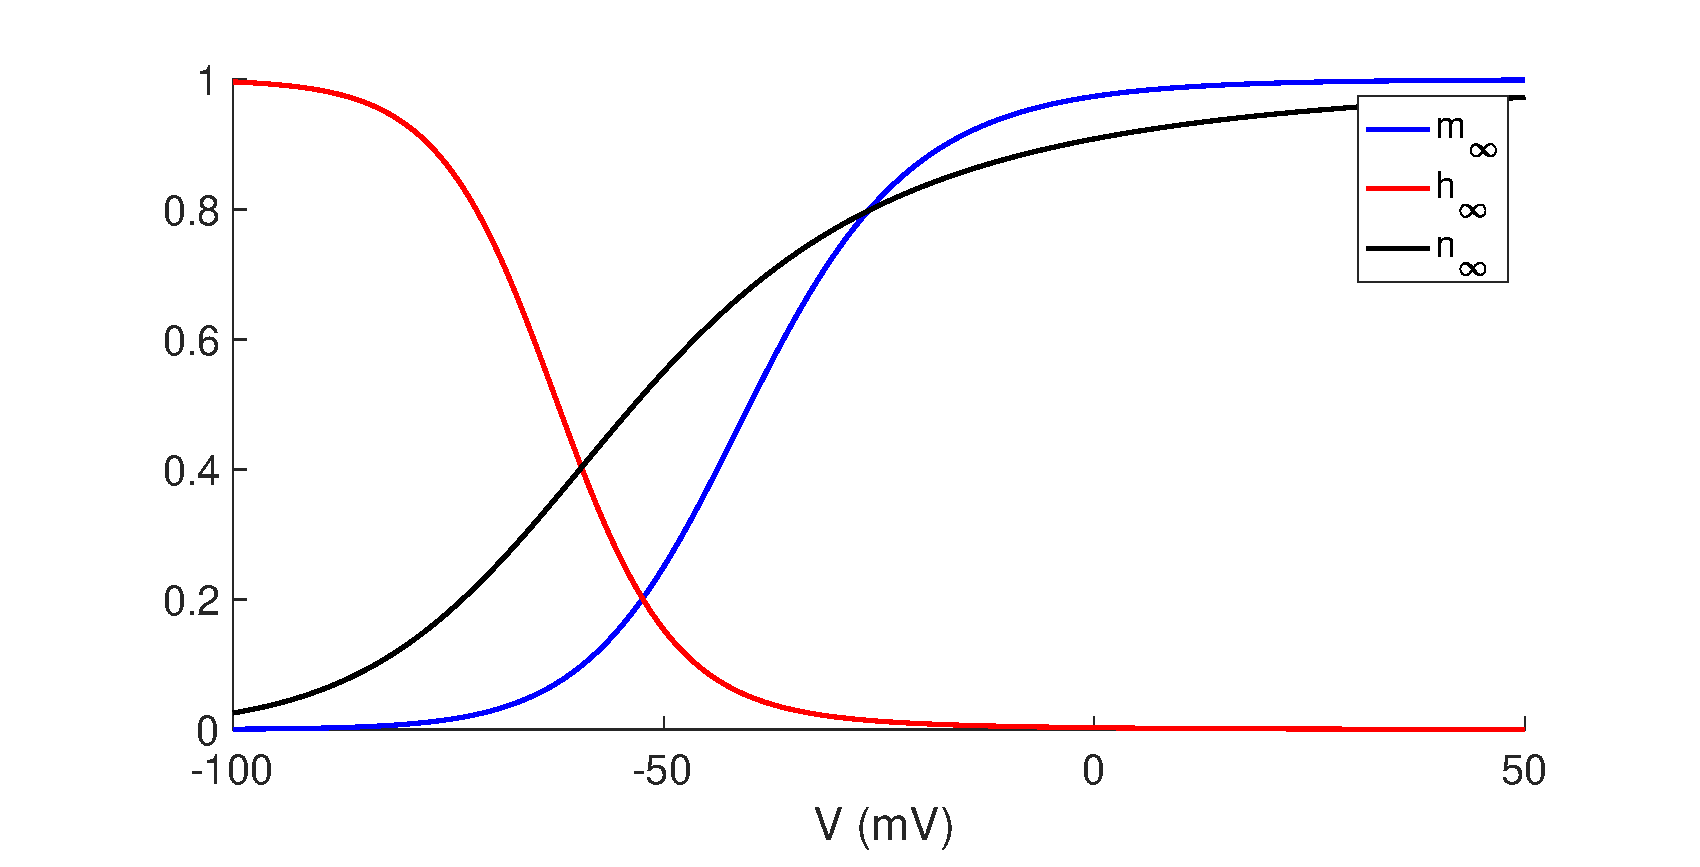
\includegraphics[width=1\linewidth]{Images/photo1_1.eps}
\end{center}
  \end{minipage} 
  \begin{minipage}{0.5\linewidth}
  \begin{center}
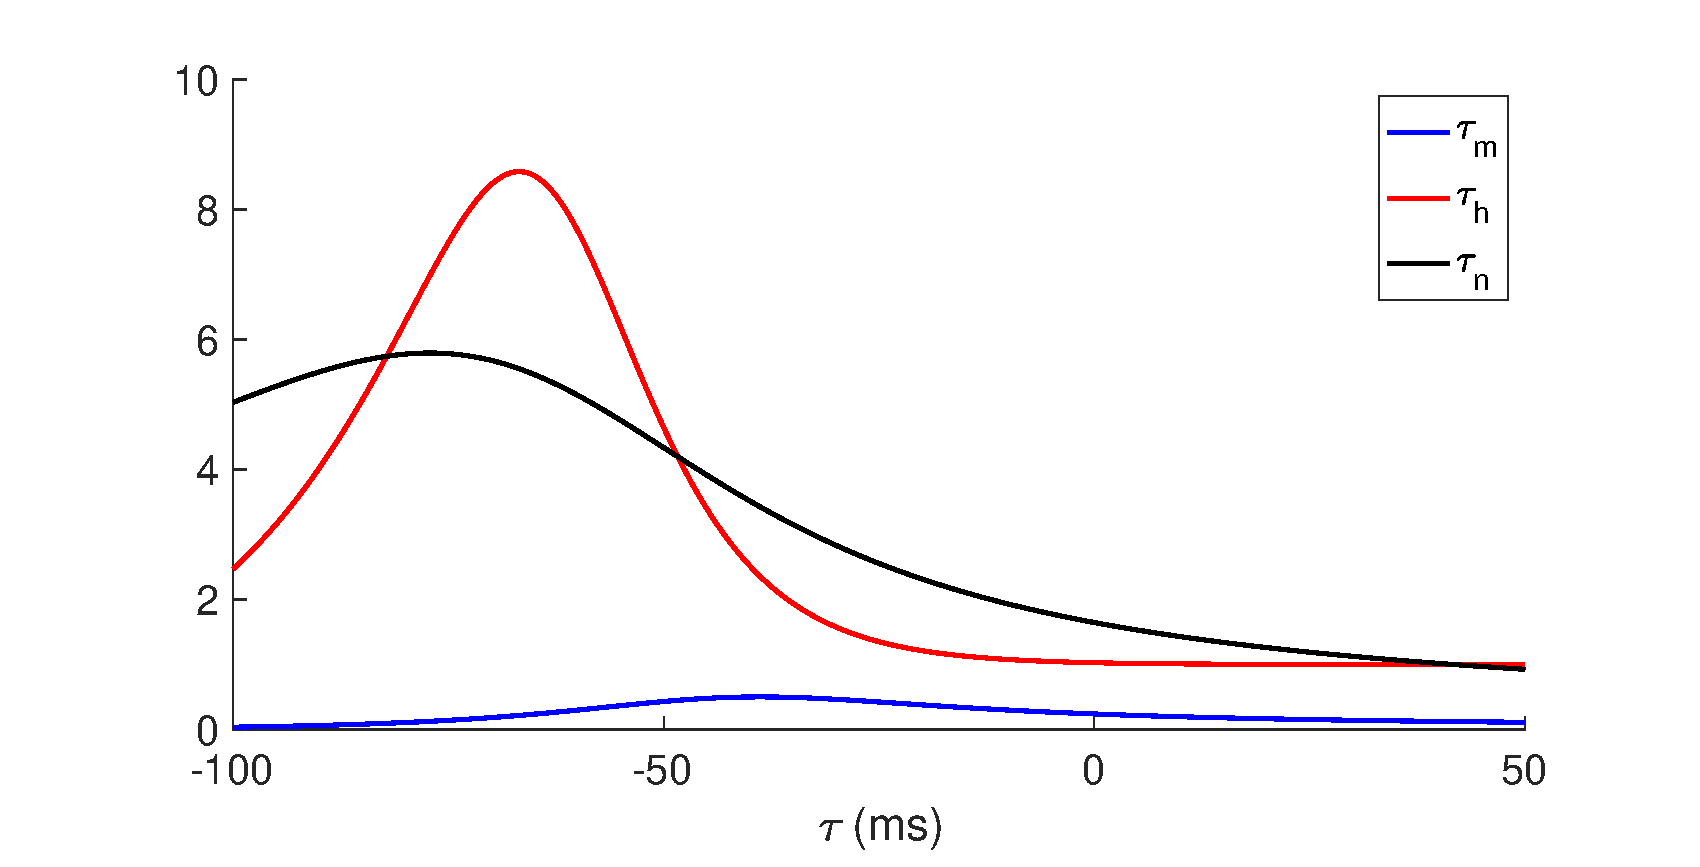
\includegraphics[width=1\linewidth]{Images/photo1_2.eps}
\end{center}
  \end{minipage} 
  \caption{\textbf{Steady state activation/inactivation curves and time constants in the Hodgkin-Huxley model.} Left: steady state activation/inactivation curves. Right: activation/inactivation time constants.}
  \label{photo1}
\end{figure}

\subsection{Conductance-Based models}
The original Hodgkin-Huxley model previously presented, was developed using data from the giant axon of the squid and conductance $Na^{+}$ and $K^{+}$ dynamics were experimentally determined for this case.

However, the same formalism can be used to study most neurons with different conductance dynamics. Neuron models based on these ideas are known as conductance-based models. Conductance-based models can reproduce with quite accuracy the complex behaviour of real neurons.

Each conductance is associated with a reversal potential $E$, a maximal conductance $\bar{g}$, integer exponents $p$ and $q$, and gating variables $m$ and $h$. Each ionic current is described as

\begin{equation}
    I_{ion} = \bar{g}m^{p}h^{q}(V-E)
\end{equation}

Gating variables $m$ and $h$ are known respectively as activation and inactivation variables and satisfy a first order differential equation of identical form

\begin{equation}
    \frac{dX}{dt} = \frac{X_{\infty}(V)-X}{\tau_{X}}
\end{equation}

where $X = m,h$ represents a generic gating variable. Functions $X_{\infty}(V)$ and $\tau_{X}$ are determined from experimental data for each specific neuron.

Gating variables represent the opening and closing dynamics of gating channels, and their dynamics can also be expressed in terms of the channel opening ($\alpha_{X}$) and closing rates $(\beta_{X})$

\begin{equation}
    \frac{dX}{dt} = \alpha_{X}(1-X) - \beta_{X}X
\end{equation}

Research on conductance-based models focus on understanding how the properties of membrane and synaptic conductances give rise to different neural responses. When different ionic currents give rise to similar activity, degeneracy emerge. Thus, conductace-based models have been widely used in the study of the degeneracy problem.

\subsubsection{An example of a conductance-based model}
As an example of a single-compartment, conductance-based biophysical model, we present the model for cells in the internal segment of the globus pallidus (GPi), \cite{Rubin2004,Terman2002} which is used  in the \textit{STN-GPe-GPi-TC} network for GPi cells.

The model includes spiking producing currents sodium ($I_{Na}$) and potassium ($I_{K}$) currents and a leak current ($I_{L}$). Each cell contains also the following types of ionic currents: a calcium activated, voltage-independent afterhyperpolarization potassium current ($I_{AHP}$), a high threshold calcium current ($I_{Ca}$) and a low threshold T-type calcium current ($I_{T}$). These additional ionic currents, based on experimental data, allows the model to reflect $\textit{in vivo}$ firing patterns and they are responsible of most firing properties displayed by GPi cells.

In addition GPi cells receives synaptic current ($I_{syn}$) and applied current ($I_{app}$). For the moment we neglect the synaptic current ($I_{syn}$) ans focus on the single cell model. Overall, each GPi cell is described by a set of five differential equation of the form

\begin{equation}
    C\frac{dV}{dt} = -I_{L} - I_{K} - I_{Na} - I_{T} - I_{Ca} - I_{AHP} + I_{app}
\end{equation}

\begin{equation}
    \frac{dX}{dt} = \Phi_{X} \left( \frac{X_{\infty}(V)-X}{\tau_{X}(V)} \right), \hspace{0.5cm} X=n,h \text{ and } r
\end{equation}
\begin{equation}
    \frac{d[Ca]}{dt} = \varepsilon(-I_{L}-I_{T}-K_{Ca}[Ca])
    \label{ref1}
\end{equation}

The leak current and voltage-dependent currents are given by the Hodgkin-Huxley formalism by

\begin{equation}
    I_{L} = \bar{g}_{L}(V-E_{L})
\end{equation}
\begin{equation}
    I_{K} = \bar{g}_{k}n^{4}(V-E_{K})
\end{equation}
\begin{equation}
    I_{Na} = \bar{g}_{k}m_{\infty}^{3}(V)h(V-E_{Na})
\end{equation}
\begin{equation}
    I_{T} = \bar{g}_{T}a_{\infty}(V)r(V-E_{T})
\end{equation}
\begin{equation}
    I_{Ca} = \bar{g}_{Ca}s_{\infty}^{2}(V)(V-E_{Ca})
\end{equation}

In addition the model presents a calcium-dependent current, the afterhyperpolarization potassium current (AHP) of the form

\begin{equation}
    I_{AHP} = \bar{g}_{AHP}(V-E_{AHP})\left(\frac{[Ca]}{[Ca]+k_{1}} \right)
\end{equation}

where the intracellular concentration of calcium ions ($Ca^{2+}$) is given by Eq. (\ref{ref1}).

Fig. (\ref{photo2}) shows voltage traces for GPi neurons for different levels of applied currents. GPi can fire rapid periodic spikes with sufficient applied current. They also display bursts of activity when subjected to small constant hyperpolarization current.

\begin{figure}[h]
  \begin{minipage}{0.5\linewidth}
  \begin{center}
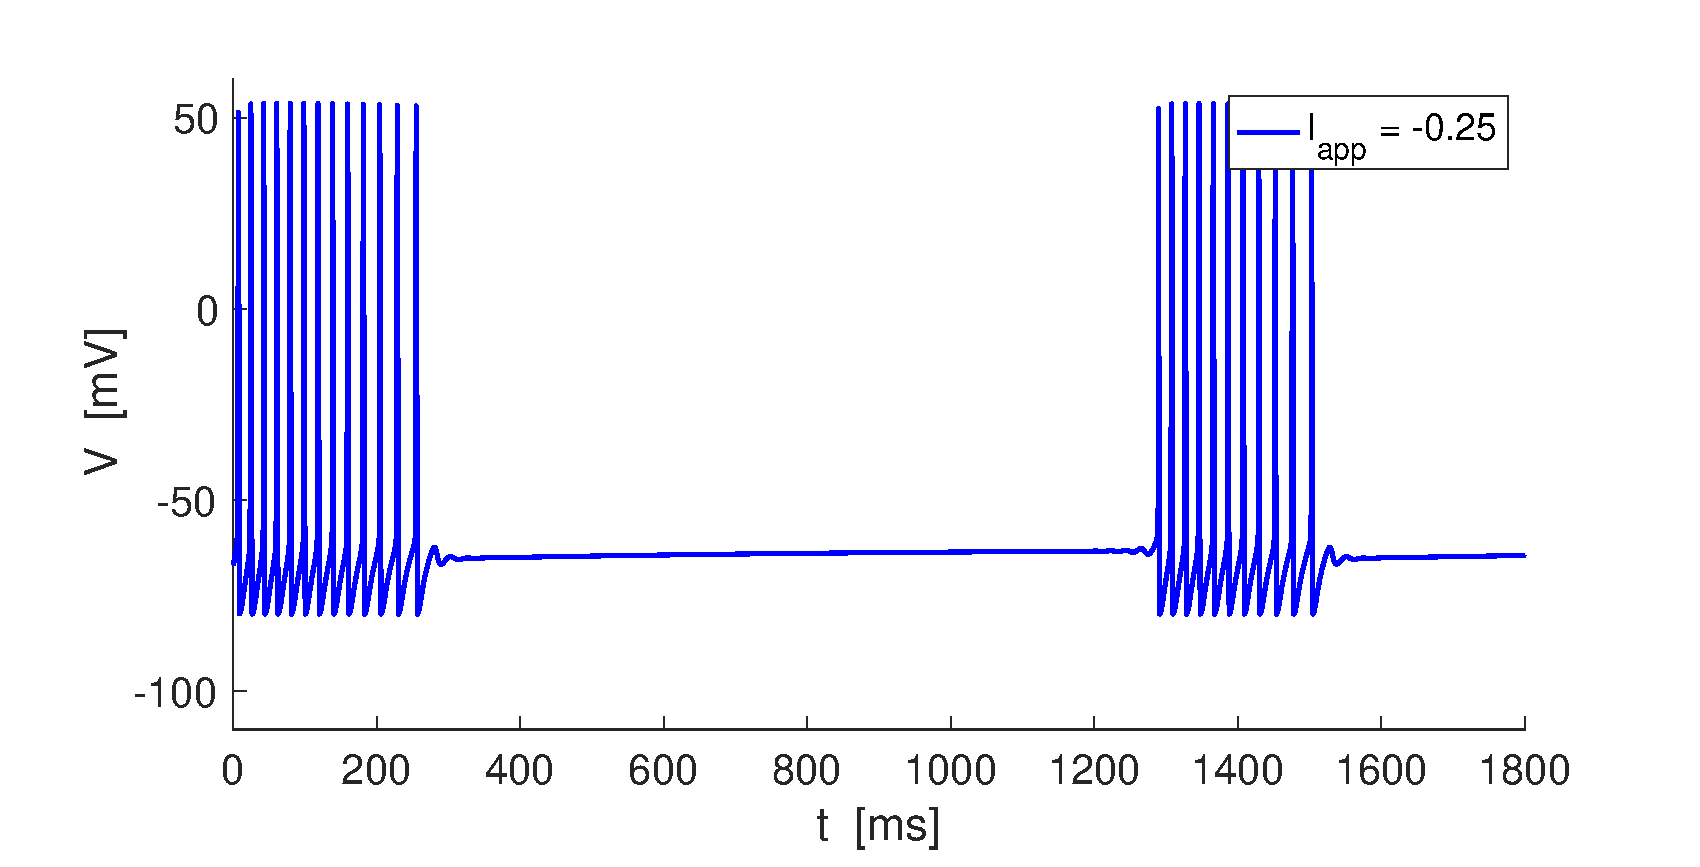
\includegraphics[width=1\linewidth]{Images/photo2_1.eps}
\end{center}
  \end{minipage} 
  \begin{minipage}{0.5\linewidth}
  \begin{center}
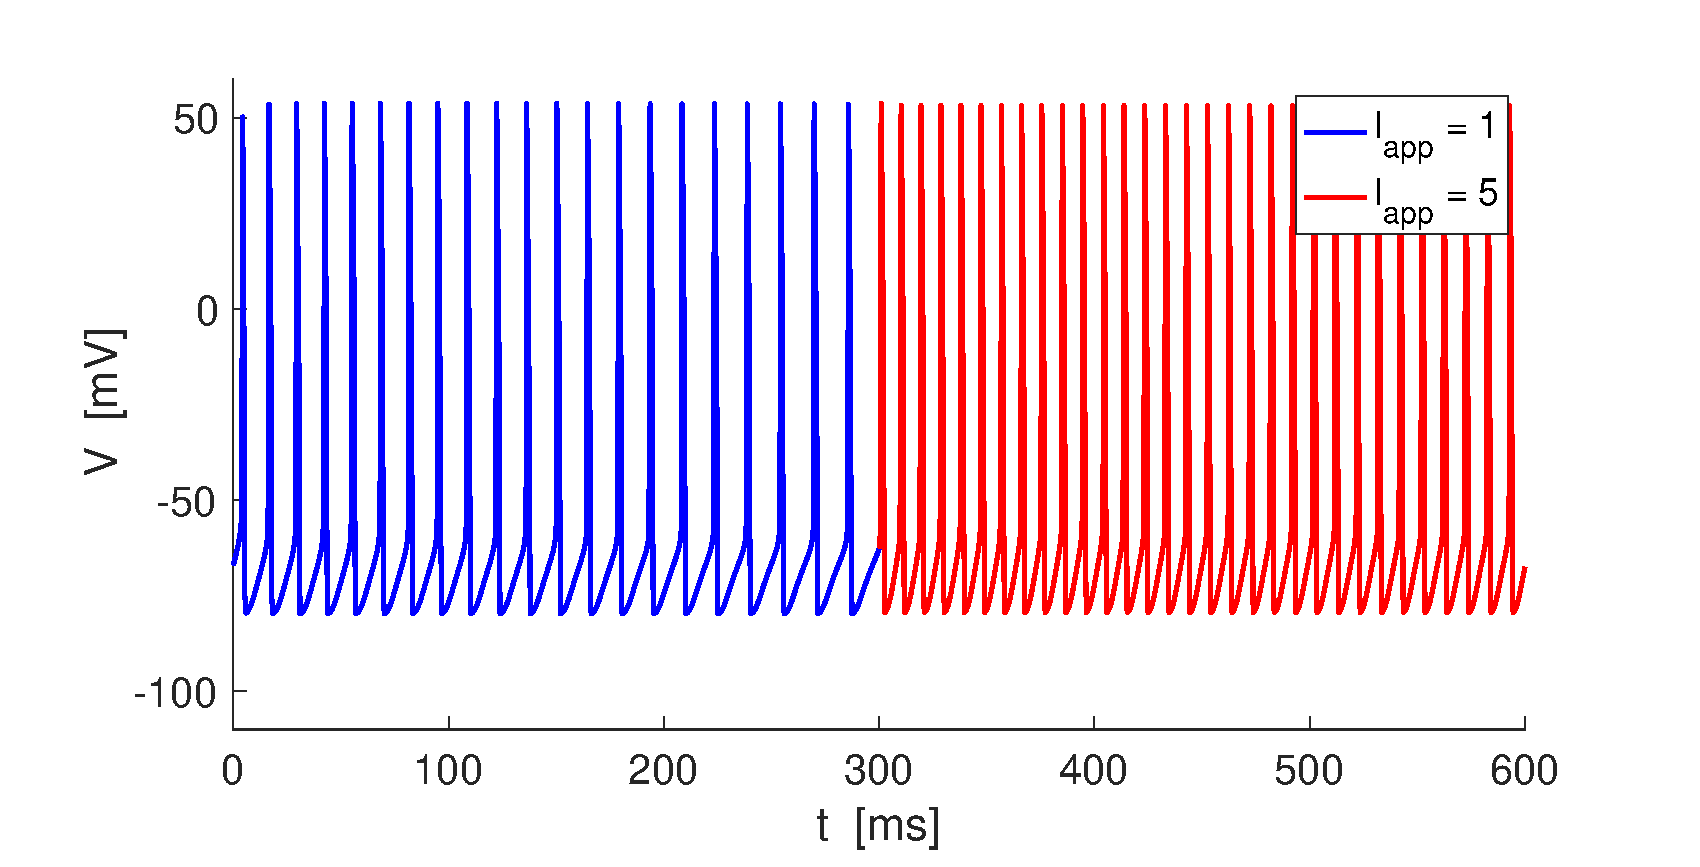
\includegraphics[width=1\linewidth]{Images/photo2_2.eps}
\end{center}
  \end{minipage} 
  \caption{\textbf{Voltage traces for GPi cells for different levels of applied current} Left: GPi cells fire burst of spikes for small negative applied current. Right: GPi cells fire rapid periodic spikes under positive input.}
  \label{photo2}
\end{figure}


\subsection{Reduced models}
Most conductance-based models involve a large number of dynamic variables which make it difficult to carry out a mathematical analysis. Reduced models, in which the number of dynamic variables has been reduced, are of mathematical interest since powerful dynamical system tools such as phase-plane analysis can be performed.

There exist several techniques that can be used to reduce high-dimensional neuron models. For instance, when the voltage-dependent time constant for a particular gating variable ($\tau_{X}$) is much smaller than the rest, the gating variable can be replaced by its stationary solution ($X_{\infty}$) and the dimensionality of the model is reduced by one.

Despite of the importance of these techniques, we will merely present a couple of two-variable models, which have been widely used across computational neuroscience community. Moreover both models presented here, have been used in the study of the degeneracy problem, \cite{Rot,Iii2019}, what make them relevant to our work.

\subsubsection{The Morris-Lecar model}
One of them is the well-known Morris and Lecar model (ML model). Although its simplicity, it is able to exhibit many of the properties displayed by neurons.

The ML model has three channels: a potassium channel, a leak and a calcium channel and it is assumed that the calcium current depends instantaneously on the voltage. The ML equations have the form

\begin{equation}
    C\frac{dV}{dt} = - \bar{g}_{L}(V-E_{L}) - \bar{g}_{K}n(V-E_{K}) - \bar{g}_{Ca}m_{\infty}(V)(V-E_{Ca})
\end{equation}
\begin{equation}
    \frac{dn}{dt} = \frac{n_{\infty}-n}{\tau_{n}(V)}
\end{equation}

where

\begin{equation}
    m_{\infty}(V) = \frac{1}{2}\left(1+tanh((V-V_{2})/V_{2}) \right)
\end{equation}
\begin{equation}
    \tau_{n}(V) = \frac{1}{cosh((V-V_{3})/(2V_{4}))}
\end{equation}
\begin{equation}
 n_{\infty}(V) = \frac{1}{2}\left(1+tanh((V-V_{3})/V_{4}) \right)
\end{equation}

Here, parameters $V_{1}$, $V_{2}$,$V_{3}$ and $V_{4}$ are parameters chosen to fit experimental data.

\subsubsection{The Fitzhugh-Nagumo model}
The second model is the Fitzhugh-Nagumo model (FHN model), \cite{Rot}. In fact, we present here a slightly different version from the original FHN model, \cite{4066548,Fitzhugh1960}. The model is given by 

\begin{equation}
    \frac{dV}{dt} = -hV^{3} + aV^{2} - w
\end{equation}
\begin{equation}
    \frac{dw}{dt} = \varepsilon(\alpha v-\lambda-w)
\end{equation}

where variables $V$ and $w$ describe the voltage and the gating variable, respectively. Furthermore,  parameters $h,a,\alpha, \varepsilon >0$ while parameter $\lambda$ can be any real number.

As well as the ML model, the FHN captures many of the properties of more complex biophysical models. In contrast, unlike the ML model, the FHN model is a simplified neuron model which do not have a biophysical derivation, but shares most mathematical properties with biophysical neuron models.

\section{Synaptic dynamics models}
In building a neuron cell network, it is necessary to determine how neurons are coupled to each other. The main difference between electrical and chemical synapses is that electrical synapses involve a continuous communications between neurons, in contrast with chemical synapses, when the communication is produced when an action potential reach the presynaptic neuron.

\subsection{Electrical synapses}
When cells communicate each other via tight junctions between their membranes, they are synaptically connected via electrical or gap junctions. The synaptic current of the postsynaptic neuron due to an electrical synapse is given by
\begin{equation}
    I_{e} = \bar{g}_{e}(V_{pre}-V_{post})
\end{equation}
where $V_{pre}$ and $V_{post}$ are the corresponding voltages of presynaptic and postsynaptic neurons respectively.

\subsection{Chemical synapses}
At a chemical synapses, presynaptic firing results in the release of transmitter. Binding to receptors on the postsynaptic neuron leads to the opening of ion channels which induces a change in the membrane conductance of the postsynaptic neuron at the site of the synapse. Traditionally, synapses are classified as excitatory or inhibitory, depending on whether they tend to depolarize or hyperpolarize a neuron (enhance firing or not).

The synaptic current for the postsynaptic neuron can be written 

\begin{equation}
    I_{s} = \bar{g}_{s}s(E_{s}-V_{post})
\end{equation}

where $E_{s}$ is the synaptic reversal potential and $\bar{g}_{s}$ the maximal synaptic conductance. The synaptic variable $s$ is related with both the probability that transmitter is released by the presynpatic neuron when it receives the arrival of an action potential and the probability that a postsynaptic channel opens, given that the transmitter was released by the presynaptic neuron.

In a simple synaptic model, it is assumed a transmitter release when an action potential reach the presynaptic neuron. Then, the change with time of the probability that a postsynaptic channel opens can be expressed as

\begin{equation}
    \frac{ds}{dt} = \alpha_{s}(1-s)-\beta_{s}s
\end{equation}

where $\beta_{s}$ determines the closing rate of the channel and is usually assumed to be constant. The opening rate, $\alpha_{s}$, however, has a higher dependence on transmitter concentration. When an action potential reaches the presynaptic neuron, the transmitter concentration rises and $\alpha_{s}$ increases rapidly, causing $s$ to increase. Following the release of transmitter there is a rapid reduction of the transmitter concentration.

\subsubsection{An example of a chemical synapse}
Considering the \textit{STN-GPe-GPi-TC} network model and, as an example of a chemical synapses, we summarize how synaptic currents were modeled in this realistic network.

For instance, synaptic current from a GPe cell (e) to a GPi cell (i) is given by

\begin{equation}
    I_{e\rightarrow i} = \bar{g}_{e\rightarrow i}s_{e}(V_{e}-E_{e\rightarrow i})
\end{equation}

The synaptic variable $s_{e}$ satisfies a first order differential equation of the form

\begin{equation}
    \frac{ds_{e}}{dt} = \alpha_{e}(1-s_{e})H_{\infty}(V_{e}-\theta_{T}) - \beta_{e}s_{e}
    \label{ref2}
\end{equation}

where $H_{\infty}$ is a smooth approximation of the Heaviside function. Here, $\alpha_{e}$ and $\beta_{e}$ represent the rates at which the synapse turn on and turn off and $\theta_{T}$ is a voltage threshold for the presynaptic voltage neuron. Tab. (\ref{t1}) shows the synaptic parameter values.

\begin{table}[h]
	\begin{tabularx}{\textwidth}{X | X | X}
		%\hline
		$\alpha_{e}$		& $\beta_{e}$			& $\theta_{T}$  \\ \hline
		1			& 0.1			& -20				\\ 
	\end{tabularx}
	\caption{Synaptic parameter values.}
	\label{t1}
\end{table}

Figure (\ref{photo3}) shows the synaptic conductance as a function of time due a single presynaptic spike on a GPe cell. We note that synaptic variable $s_{e}$ increases when presynaptic GPe voltage is higher than the voltage threshold $\theta_{e}$. It starts to decrease when the action potential terminates and voltage is lower than the voltage threshold $\theta_{T}$.

\begin{figure}[h]
  \begin{minipage}{0.5\linewidth}
  \begin{center}
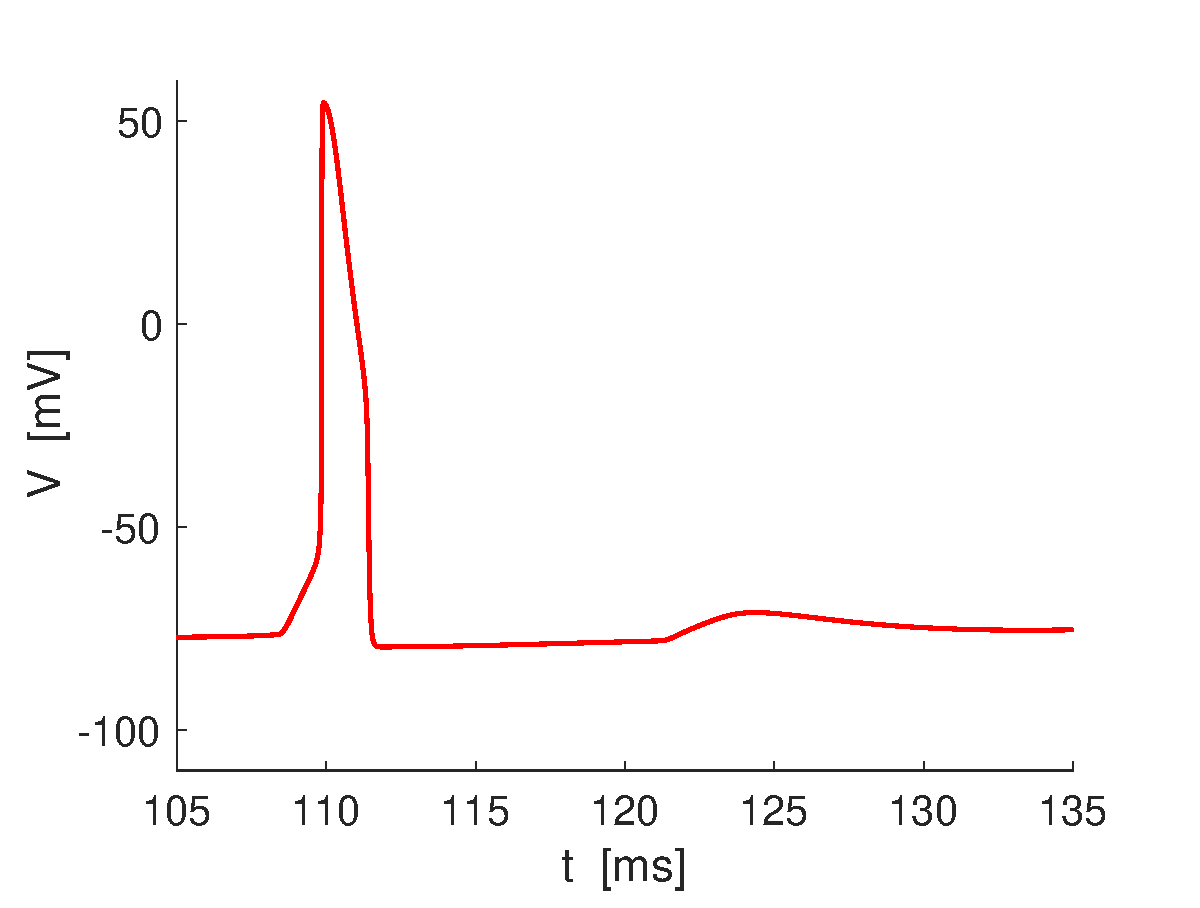
\includegraphics[width=1\linewidth]{Images/photo3_1.eps}
\end{center}
  \end{minipage} 
  \begin{minipage}{0.5\linewidth}
  \begin{center}
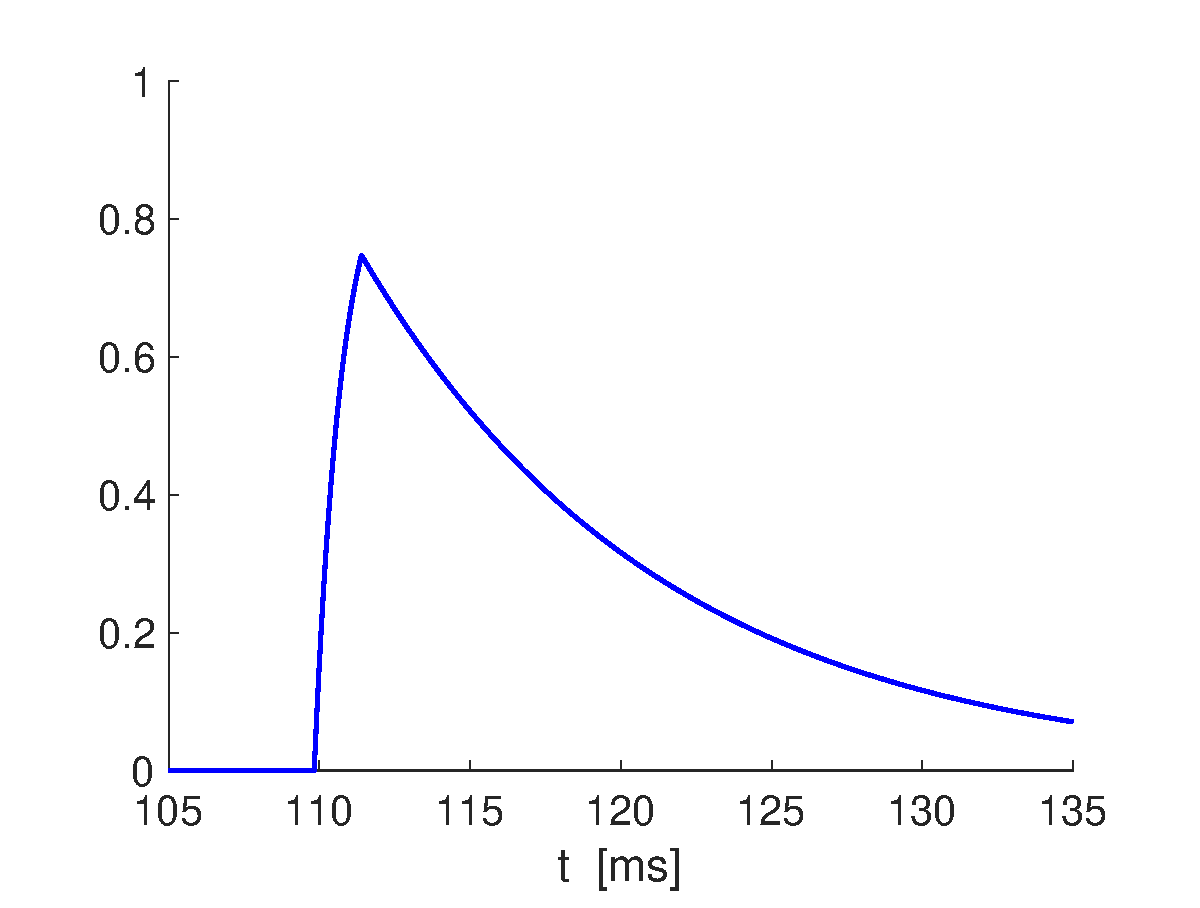
\includegraphics[width=1\linewidth]{Images/photo3_2.eps}
\end{center}
  \end{minipage} 
  \caption{\textbf{Synaptic conductance model in the \textit{STN-GPe-GPi-TC} network.} Left: single presynaptic spike on a GPe cell. Right: conductance due to a single spike on presynaptic GPe cell (left).}
  \label{photo3}
\end{figure}



\section{Mathematical Models for Neuronal Networks}
One described single cell models and synaptic models, we describe some mathematical models for neuron networks.

Apparently, the most direct way to simulate neural network is to synaptically connect model spiking neurons, such as conductance based models. This is how mathematical models for neuronal networks are built in this section. However, we notice the existence of other neural network models, such as Firing-Rate models, which are widely used in computational neuroscience. Firing-Rate models, instead of voltage, use as an output the firing rate, which is a measure of the number of spikes generated per unit of time.

Despite the importance of Firing-Rate models in computational neuroscience, we focus on neuronal network built connecting single neuron spiking models, since mathematical networks considered in this work are inspired by these type of neural networks.

We note that network properties depends on individual cells, synaptic connections between cells and the network architecture. Networks architectures, such as random or structured are possible in networks involving a large number of neurons.

In order to illustrate neural network models, we build two-neuron electrically and chemically fully connected networks. Without loss of generality, we consider a general two-variable neuron model to describe the behaviour of each neuron in the network with general form

\begin{equation}
    \frac{dV}{dt}  = f(V,w)
\end{equation}
\begin{equation}
    \frac{dw}{dt}  = g(V,w)
\end{equation}

where $V$ is the membrane potential of the cell and $w$ a channel gating variable.

\subsection{Electrical networks}
The model for a pair of mutually electrically coupled neurons is given by

\begin{equation}
    \frac{dV_{i}}{dt}  = f_{i}(V_{i},w_{i}) - \bar{g}_{j}^{i}(V_{i}-V_{j})
\end{equation}
\begin{equation}
    \frac{dw_{i}}{dt}  = g_{i}(V_{i},w_{i})
\end{equation}

where $i,j = 1 $ or $2$ and $i \neq j$ and $\bar{g}_{j}^{i}$ is the maximal conductance for synaptic current from neuron $i$ to neuron $j$.


\subsection{Chemical networks}
For chemical synapses, we assume synaptic variable $s$ satisfies a first-order differential equation of the form in Eq. (\ref{ref2}), previously studied.

The model for a pair of mutually chemically coupled neurons is then

\begin{equation}
    \frac{dV_{i}}{dt}  = f_{i}(V_{i},w_{i}) - \bar{g}_{s}^{i}s_{j}(V_{i}-E_{s}^{i})
\end{equation}
\begin{equation}
    \frac{dw_{i}}{dt}  = g_{i}(V_{i},w_{i})
\end{equation}
\begin{equation}
    \frac{ds_{i}}{dt}  = \alpha_{s}^{i}(1-s_{i})H_{\infty}(V_{i}-\theta_{T}^{i})-\beta_{s}^{i}s_{i}
\end{equation}

where $i,j = 1 $, $2$ and $i \neq j$.

Network models presented, correspond to the most general heterogeneous network, in which cells have different intrinsic parameters.
   % INCLUDE: introduction
\chapter{Previous Work on Attribute Level Sets}
\label{sec:prev}
In this section, previous work on attribute level sets on neuronal models is described. The contents of this section are mainly based on \cite{Oly,Rot,Iii2019}. 
\section{Existence of attribute level sets in complex systems}
Contribution in \cite{Oly} focus on proving the existence of attribute level sets in complex neuronal systems and networks, although results are more general and could be applied to any model based on parameters meeting certain specific requirements.

The technique is mainly based on the implicit function theorem which imposes certain conditions which need to be guaranteed. For instance, the method developed can only applied to first-order differentiable (on variables and parameters) models.

Using the implicit functions theorem, they are able not only to prove the existence of attribute level sets near a generic point on parameter space, but also to compute the exact compensatory function (attribute level sets) on parameter space, using the linear approximation also provided by the theorem. They propose an algorithm to compute exact compensatory covariations.

Moreover the algorithm developed was applied to a biophysical conductance-based model, consisting in two identical neurons that mutually inhibit one another. Two attribute level sets were computed on different parameter spaces in order to illustrate the method.

On the one hand, they considered the $\bar{g}_{h}-\bar{g}_{SynS}$ parameter space. Here, $\bar{g}_{h}$ is the maximal conductance of a hyperpolarization-activated current ($I_{h}$) and $\bar{g}_{SynS}$ the maximal conductance of the chemical synapses current. They found level sets on this parameter space preserving the burst period (T). Bursting is characterized by a silent phase alternated with an active phase of rapid and spike-like oscillations. Fig. (\ref{photo4})-Left shows an example of such an attribute level set.

\begin{figure}[h]
\centering
\begin{minipage}{0.35\linewidth}
  \begin{center}
\includegraphics[width=1\linewidth]{Images/photo4_1.png}
\end{center}
  \end{minipage} 
  \begin{minipage}{0.4\linewidth}
  \begin{center}
\includegraphics[width=1\linewidth]{Images/photo4_2.png}
\end{center}
  \end{minipage} 
  \caption{\textbf{Example of 1-dimensional level sets on the $\bar{g}_{h}-\bar{g}_{SynS}$  and $\bar{g}_{h}-\bar{g}_{SynS}-\eta$ parameter spaces.} Left: level set preserving the burst period (T) on the $\bar{g}_{h}-\bar{g}_{SynS}$ parameter space. Right: level set preserving both the burst period (T) and the intraburst spike frequency (f) on the $\bar{g}_{h}-\bar{g}_{SynS}-\eta$ parameter space. Figures taken from \cite{Oly}.}
  \label{photo4}
\end{figure}

On the other hand, the also look for level sets on the $\bar{g}_{h}-\bar{g}_{SynS}-\eta$ parameter space preserving both the burst period (T) and the intraburst spike frequency (f). Here, $\eta$ represents a scaling factor for the inactivation time constant $\tau_{h,CaS}$ of a slowly inactivating calcium low-threshold current $I_{CaS}$. Fig. (\ref{photo4})-Right shows an example of such an attribute level set.

Based on the implicit theorem, they also predict that if $m$ attributes are preserved on a given level set (computed with the algorithm proposed) in a $n$-dimensional parameter space, the level set has dimension $n-m$. 

\section{Compensatory mechanisms for level set generation}
In \cite{Rot}, they used two-dimensional neuron models with different level of complexity, to study the compensatory mechanisms leading to period and duty cycle (DC) level sets. DC is defined as the fraction of the period for which the oscillation is above half its amplitude.

Their work focus on exploiting mathematical phase plane analysis and $V$-speed diagrams to see differences between them along different points within the same attribute level set and, in this way, understand the compensatory mechanisms leading to the generation of attribute level sets.

As an example, Fig. (\ref{photo5})-Left shows period level sets on the $\lambda-\alpha$ parameter space on the FHN model. In addition, Fig. (\ref{photo5})- Middle shows $V-$ (red) and $w-$ (green) nullclines as well as the trajectories (blue) in the phase plane for two different points on a fixed period level set (normal and dashed lines), and Fig. (\ref{photo5})- Right shows the $V$-speed graph as a function of V for the same two points in the level set.

\begin{figure}[h]
\centering
        \begin{minipage}{0.33\linewidth}
            \begin{center}
                \includegraphics[width=1\linewidth]{Images/photo5_1.png}
            \end{center}
        \end{minipage} 
        \begin{minipage}{0.3\linewidth}
            \begin{center}
                \includegraphics[width=1\linewidth]{Images/photo5_2.png}
            \end{center}
        \end{minipage} 
    \begin{minipage}{0.29\linewidth}
        \begin{center}
            \includegraphics[width=1\linewidth]{Images/photo5_3.png}
        \end{center}
    \end{minipage} 
  
  \caption{\textbf{Period level sets on the $\lambda-\alpha$ parameter space, a phase-plane plot and a $V-$speed graph for the FHN model.} Left: period (T) level sets on the $\lambda-\alpha$ parameter space. Middle: an example of a phase-plane plot. Normal and dashed lines represent two different points within the same period level set. Red lines represents $V$-nullclines whereas green lines $w$-nullclines. Trajectories are in blue. Right: an example of a $V-$speed graph as a function of voltage $V$. Figures taken from \cite{Rot}.}
  \label{photo5}
\end{figure}

\section{Connecting cells within the same level set}
In \cite{Iii2019}, the ML model and a reduced two-dimesional conductance-based model (the Calcium/H -current oscillatory model) were used to form different homogeneous (identical cells) and heterogeneous (non-identical cells, but within the same level set) networks with electrical and chemical synapses. Significant differences between electrical and chemical networks in both models were found.

Cells were connected in a pairwise manner to produce different homogeneous and heterogeneous networks. Synaptic strength in networks was controlled by one parameters $G_{ElectSyn}$ and $G_{ChemSyn}$ in electrical and chemical networks respectively.

They show how electrical networks with different synaptic strength were able to preserve the individual cell frequency. In contrast, in synaptic networks they show either a decrease (Calcium/H -current model) or increase (ML model) in the individual cell frequency as the chemical synaptic strength increases.

Fig. (\ref{photo6}) shows the results in networks considering the Calcium/H -current model.

\begin{figure}[h]
\centering
\includegraphics[width=0.8\linewidth]{Images/photo6_1.png}
  \caption{\textbf{Change in cell frequencies as per the increase in synaptic strengths.} A1-A2: electrical networks; B1-B2: chemical networks; A1-B1: homogeneous networks (identical cells); A2-B2: heterogeneous networks (cells within the same frequency level set). Figure taken from \cite{Iii2019}.}
  \label{photo6}
\end{figure}

Clearly, in chemical networks cells become part of a new network level set when connected. Regarding electrical networks, they show that electrical synapses was able to maintain the individual cell frequency, but other attributes, such as the amplitude, were not studied. Therefore, it is not known whether or not individual attribute level sets are preserved as well.

It is worth noting that, since different electrical synapses conductances preserve the network frequency, they constitute network frequency level sets on the connectivity parameter space. However, the connectivity parameter space considered here, as well as the network architecture, might be too simplified. 

Nevertheless, this work is a good starting point to the work developed in this project for two mainly reasons. Firstly, we ask if individual level sets are preserved when cells are electrically connected. Secondly, we would like to study more in detail network level sets on the connectivity parameter space in more complex networks architectures with higher dimensional parameter spaces. We will develop these ideas on a simplified mathematical network model.
   % INCLUDE: introduction
\chapter{Methods}
\label{sec:methods}
In this section, the so-called $\Lambda \Omega$ systems are introduced. In addition, a special class of $\Lambda \Omega$ systems, the $\Lambda \Omega_{2}$ system, is presented and degeneracy is characterized on this particular system. We also establish how $\Lambda \Omega_{2}$ systems are interconnected in order to form $\Lambda \Omega_{2}$ networks, where the degeneracy problem will be studied.

Important concepts such as attribute level sets or total-degeneracy are also defined in this section.   

\section{$\Lambda \Omega$ Systems}
$\Lambda \Omega$ systems are simple oscillatory systems. Equations describing $\Lambda \Omega$ systems have the general form

\begin{equation}
    \frac{dx}{dt} = \Lambda(r)x-\Omega(r)y
    \label{e1}
\end{equation}
\begin{equation}
    \frac{dy}{dt} = \Omega(r)x+\Lambda(r)y
    \label{e2}
\end{equation}
with
\begin{equation}
r^{2}=x^{2}+y^{2}
\label{e3}
\end{equation}

where x and y are state variables and t is time. $\Lambda$ and $\Omega$ are real functions of single variable. The system is linear only if functions $\Lambda$ and $\Omega$ are constants. Otherwise, $\Lambda \Omega$ systems are a class of non-linear system of ordinary differential equations.

They have been extensively used as the kinetics in the study of wave phenomena in reaction diffusion models, \cite{Kopell1973}. These class of reaction diffusion systems have the advantage that explicit analytic solutions can be written down. However, we use the so-called $\Lambda \Omega$ systems as a class of non-trivial mathematical oscillators.

In \cite{LeonGlass2001}, $\Lambda \Omega$ systems are proposed as simple models useful to study synchronization of physiological oscillators, for example in populations of cells that generate the heart beat or gamma and beta rhythms in the brain.
They have also been used as mathematical models for central pattern generators \cite{Murray2002}, neural networks which exhibit rhythmic oscillations and do not require any external input to generate them.

It is convenient to study these systems in polar coordinates in the state space. A change of coordinates, from Cartesian to Polar

\begin{equation}
    x = r\cos(\theta) \hspace{0.5cm} \text{and} \hspace{0.5cm} y = r\sin(\theta)
    \label{e4}
\end{equation}

transforms system (\ref{e1})-(\ref{e2}) into

\begin{equation}
    \frac{dr}{dt} = r\Lambda(r)
    \label{e5}
\end{equation}
\begin{equation}
    \frac{d\theta}{dt} = \Omega(r)
    \label{e6}
\end{equation}

This form allows for the computation of the redius of the circular limit circle(s) as the solution(s) of

\begin{equation}
    \Lambda(\bar{r}) = 0
    \label{e7}
\end{equation}

We notice that a limit circle of radius $\bar{r}$ is stable if and only if $\Lambda(\bar{r})<0$. More stability details depend on functions $\Lambda(r)$ and $\Omega(r)$.

\subsection{$\Lambda \Omega_{2}$ Systems}
$\Lambda \Omega$ systems of order two ($\Lambda \Omega_{2}$) correspond to the following quadratic choices for $\Lambda(r)$ and $\Omega(r)$

\begin{equation}
    \Lambda(r) = \lambda - br^{2} \hspace{0.5cm} \text{and} \hspace{0.5cm} \Omega(r) = \omega + ar^{2}
    \label{e8}
\end{equation}

These functions belong to a specific class of $\Lambda$ and $\Omega$ functions introduced in \cite{Blowey2005,Garvie2005}, where they considered arbitrary power of the radius and performed an exhaustive mathematical and numerical analysis of these $\Lambda \Omega$ type oscillatory reaction diffusion equations.

Therefore, $\Lambda \Omega$ systems of order two ($\Lambda \Omega_{2}$), are given by Eqs. (\ref{e1}-\ref{e2}), when functions $\Lambda$ and $\Omega$ take the form in Eq. (\ref{e8}).

$\Lambda \Omega_{2}$ systems have a set of four parameters: $\lambda$, $b$, $\omega$ and a. As we study the degeneracy problem on networks composed by units of $\Lambda \Omega_{2}$ systems, we will refer to these parameters as the intrinsic parameters, in order to distinguish between connectivity parameters of the network and parameters from each $\Lambda \Omega_{2}$ system in the network.

$\Lambda \Omega_{2}$ systems have a single limit circle for 

\begin{equation}
    \bar{r} = \sqrt{\frac{\lambda}{b}}
     \label{e9}
\end{equation}

if $\lambda/b>0$ which is stable if and only if $b>0$. Therefore, only when parameters $\lambda$ and $b$ are both positive the system show sustained oscillations. Moreover, as parameter $\lambda$ becomes positive, the stable fixed point $(\bar{x},\bar{y})$ becomes unstable and the system undergoes a supercritical Hopf bifurcation.

Fig. (\ref{photo7}) shows the nullclines and the trajectory for a representative solution to the $\Lambda \Omega_{2}$ system. It is also shown the sinusoidal-like solutions of the state variables as a function of time.

\begin{figure}[h]
  \begin{minipage}{0.45\linewidth}
  \begin{center}
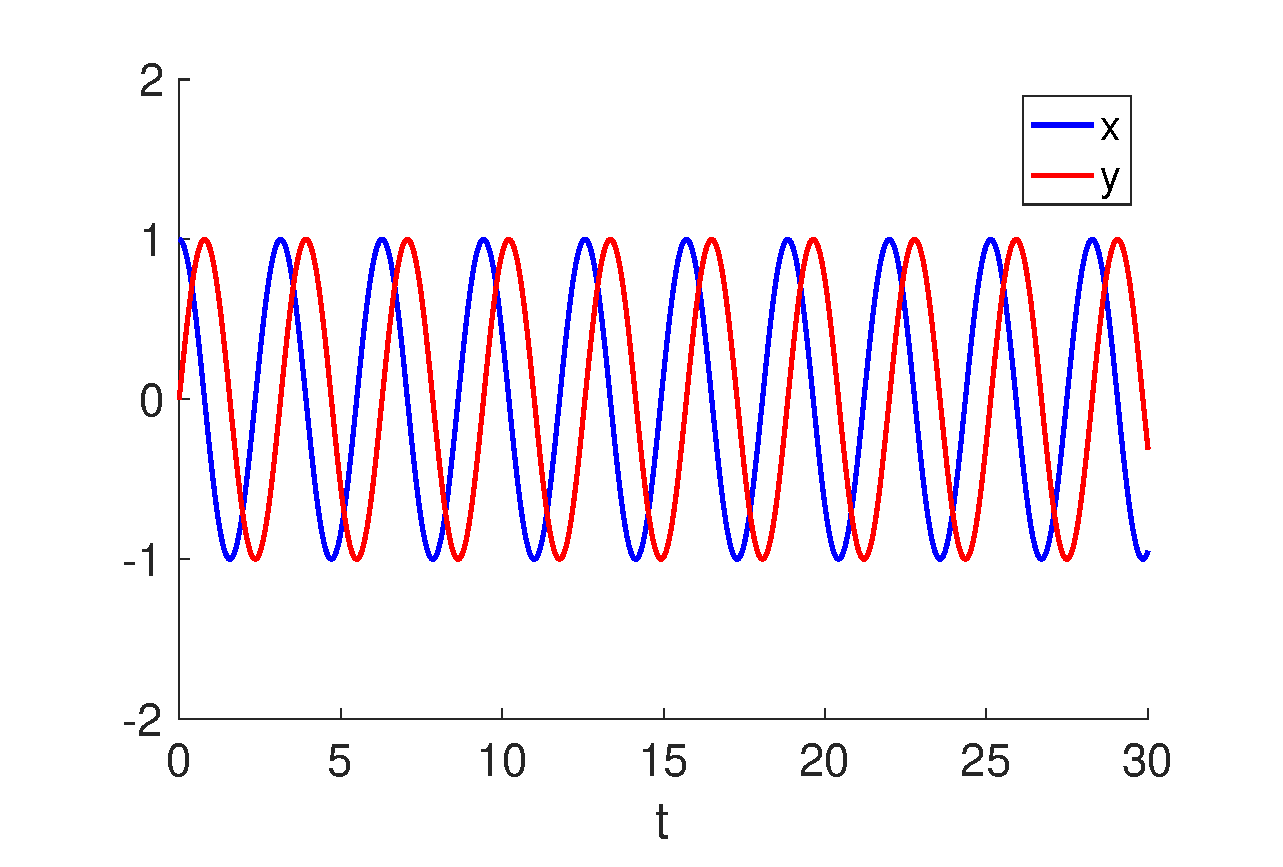
\includegraphics[width=1\linewidth]{Images/photo7_1.eps}
\end{center}
  \end{minipage} 
  \begin{minipage}{0.45\linewidth}
  \begin{center}
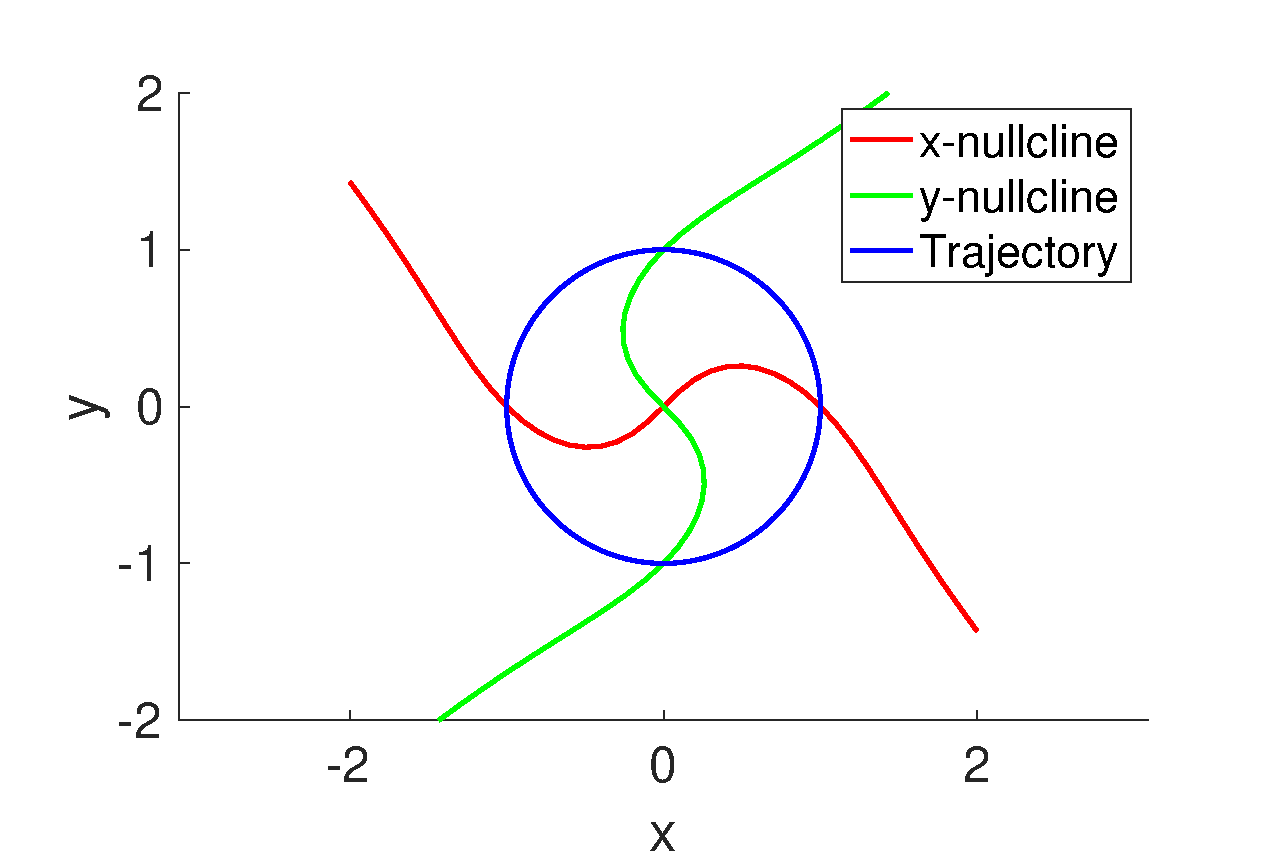
\includegraphics[width=1\linewidth]{Images/photo7_2.eps}
\end{center}
  \end{minipage} 
  \caption{\textbf{Dynamics of the $\Lambda \Omega_{2}$ systems.} Left: traces (curves of x and y as a function of t). Right: phase-plane diagram. The x- and y- nullclines are the set of points in the x-y plane that make $dx/dt=0$ and $dy/dt=0$ respectively. Parameter values: $\lambda = 1$, $b=1$, $a = 1$ and $\omega = 1$.}
  \label{photo7}
\end{figure}

Since we are interested in $\Lambda \Omega_{2}$ systems as mathematical oscillators we focus on the case when $\Lambda \Omega_{2}$ systems show a stable limit circle, towards which solutions converge in the limit of $t\rightarrow \infty$. We characterize the stationary oscillatory solutions by two attributes of the oscillatory pattern: the amplitude and frequency.

Simple theoretical oscillatory models, such as $\Lambda \Omega_{2}$ systems, are useful to study qualitative aspects of real physiological systems, from which they tend to be realistic simplifications. In this work, we consider $\Lambda \Omega_{2}$ systems as simplified models that simulate the behaviour of a neuronal cell. However, these $\Lambda \Omega_{2}$ models are too oversimplified to accurately represent a realistic neuron. Nonetheless, we shall consider the $\Lambda \Omega_{2}$ system as a toy model which would represent the behaviour of an hypothetical neuron.

In this respect, we consider variable x in Eq. (\ref{e4}) as the corresponding variable representing the voltage of an hypothetical cell modelled by a $\Lambda \Omega_{2}$ system. Furthermore, all attributes considered will characterized the oscillatory pattern of the cell voltage, i.e., variable x in the $\Lambda \Omega_{2}$ system.

\section{$\Lambda \Omega_{2}$ Networks}
The general form of the linear connectivity networks we consider is

\begin{equation}
    \frac{dx_{k}}{dt} = \Lambda_{k}(r_{k})x_{k} - \Omega_{k}(r_{k})y_{k} - \sum_{j=1}^{N}\alpha_{k,j}x_{j}
    \label{e10}
\end{equation}
\begin{equation}
    \frac{dy_{k}}{dt} = \Omega_{k}(r_{k})x_{k} + \Lambda_{k}(r_{k})y_{k}
    \label{e11}
\end{equation}

where

\begin{equation}
r_{k}^{2}=x_{k}^{2}+y_{k}^{2}
\label{e12}
\end{equation}

and $A=\{\alpha_{k,j}\}$ is the connectivity matrix. We shall call $\alpha_{k,k}$ self-connectivity parameters and $\alpha_{k,j}$ ($k \neq j$) cross-connectivity parameters.

$\Lambda \Omega_{2}$ networks and then given by Eqs. (\ref{e10})-(\ref{e11}) taking 

\begin{equation}
    \Lambda_{k}(r_{k}) = \lambda_{k} - b_{k}r_{k}^{2} \hspace{0.5cm} \text{and} \hspace{0.5cm} \Omega_{k}(r_{k}) = \omega_{k} + a_{k}r_{k}^{2}
    \label{e13}
\end{equation}

In this work, we consider $\Lambda \Omega_{2}$ networks composed by one and two units of $\Lambda \Omega_{2}$ systems. As we consider that $\Lambda \Omega_{2}$ systems represent the behaviour of an hypothetical neuronal cell, we shall refer to these networks as the self-connected cell and the two-cell network. The goal of the project is to characterize degeneracy in these two simple networks.

Based on the intrinsic parameters of the cells, we distinguish three different types of networks: homogeneous networks (cells are identical), type-I heterogeneous networks (cells belong to the same individual amplitude and frequency LS) and type-II heterogeneous networks (cells belong to different frequency and/or amplitude LS).

\section{Degeneracy and attribute level sets}
Degeneracy, in a model which involve parameters, refers to the situation where multiple sets of parameter values can produce the same observable output or attribute. In such a model, attribute level sets are defined as the set of points on parameter space for which a given attribute is constant.

In this work, we compute several attribute level sets in $\Lambda \Omega_{2}$ networks. We focus our analysis on 1 and 2-dimensional attribute level sets, embedded in 2,3 or 4-dimensional parameter spaces. We show them parametrized by one or two parameters, respectively. As in  \cite{Oly}, we shall call these parameters the compensating parameters. 

For instance, a 2-dimensional attribute level set on a 4-dimensional parameter space $(x_{1},x_{2},y_{1},y_{2})$ would be defined by two functions of the form

\begin{equation}
\begin{split}
    y_{1} = f_{1}(x_{1},x_{2})\\
    y_{2} = f_{2}(x_{1},x_{2})
    \end{split}
    \label{e14}
\end{equation}

being $x_{1}$, $x_{2}$ the compensating parameters and $y_{1}$, $y_{2}$ the compensated parameters. Furthermore, we will refer to the parametrization functions $f_{1}$, $f_{2}$ as the compensatory functions.

\subsection{Degeneracy in $\Lambda \Omega_{2}$ Systems}
Degeneracy in $\Lambda \Omega_{2}$ systems is easily characterized. Amplitude and frequency level sets can be computed analytically. We ignore the transient of solutions and characterize degeneracy for stationary oscillatory solutions.

From Eq. (\ref{e9}) amplitude level sets are the curves in the $\lambda-b$ parameter space satisfying

\begin{equation}
    \frac{\lambda}{b} = K_{a}
    \label{e16}
\end{equation}

where $K_{a}$ is a constant. Similarly, from Eqs. (\ref{e6}) and (\ref{e8}) frequency level sets are the hypersurfaces in the $\lambda-\omega-a-b$ parameter space satisfying 

\begin{equation}
    \omega+a\frac{\lambda}{b} = K_{f}
    \label{e17}
\end{equation}

where $K_{f}$ is a constant. On a given amplitude level set, the frequency level sets are the curves in $\omega-a$ parameter space satisfying

\begin{equation}
    \omega+aK_{a} = K_{f}
    \label{e18}
\end{equation}

Therefore, for all combinations of parameter values satisfying Eqs. (\ref{e16}) and (\ref{e18}) the system has the same amplitude and frequency. Moreover, along these level sets the oscillatory patterns are identical.

\subsubsection{A plausible method to disambiguate degeneracy in $\Lambda \Omega_{2}$ Systems}
Despite degeneracy in amplitude and frequency for stationary solutions, Eqs. (\ref{e16})-(\ref{e17}), the transient solution is different among degenerated stationary solutions. These differences can be used as a method to decode degeneracy in $\Lambda \Omega_{2}$ systems.

As an example, we add a perturbation to the cell voltage, $p(t)$, of the form

\begin{equation}
    p(t) = K \left(\mathcal{H}(t-t_{on})-\mathcal{H}(t-t_{off})\right)
    \label{eq1}
\end{equation}

which corresponds to a rectangular signal of amplitude $K$ beginning at instant $t_{on}$ and ending at instant $t_{off}$. The perturbed $\Lambda \Omega_{2}$ system has the form

\begin{equation}
    \frac{dx}{dt} = \lambda x - \omega y - (bx + ay)(x^{2}+y^{2}) + p(t)
    \label{eq2}
\end{equation}
\begin{equation}
  \frac{dy}{dt} = \omega x + \lambda y + (ax - by)(x^{2}+y^{2})
  \label{eq3}
\end{equation}

Perturbations are added to amplitude degenerated $\Lambda \Omega_{2}$ system in which parameters $\lambda$ and $b$ might be different, but all systems do belong to the same amplitude level set, Eq. (\ref{e16}).

We find a correspondence between the parameter $\lambda$ and the recovery time (required time to reach stationary oscillations in the system after a perturbation). Fig. (\ref{photo8}) shows the recovery time as a functions of parameter $\lambda$ for different systems belonging to the same amplitude level set ($K_{a}=1$). It is also shown the perturbed oscillatory solutions in the phase plane.

\begin{figure}[h]
\centering
  \begin{minipage}{0.45\linewidth}
  \centering
    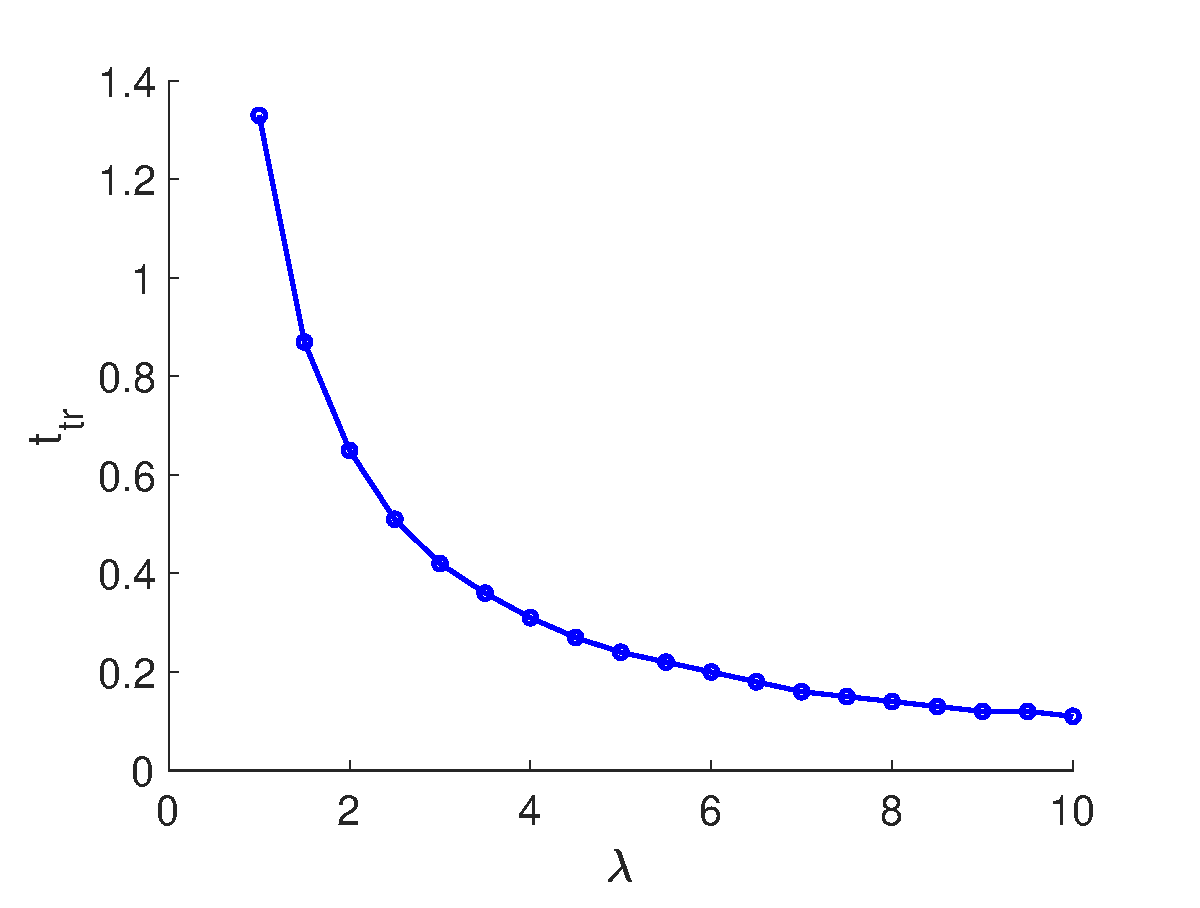
\includegraphics[width=1\linewidth]{Images/photo8_1.eps} 
  \end{minipage} 
  \begin{minipage}{0.45\linewidth}
  \centering
    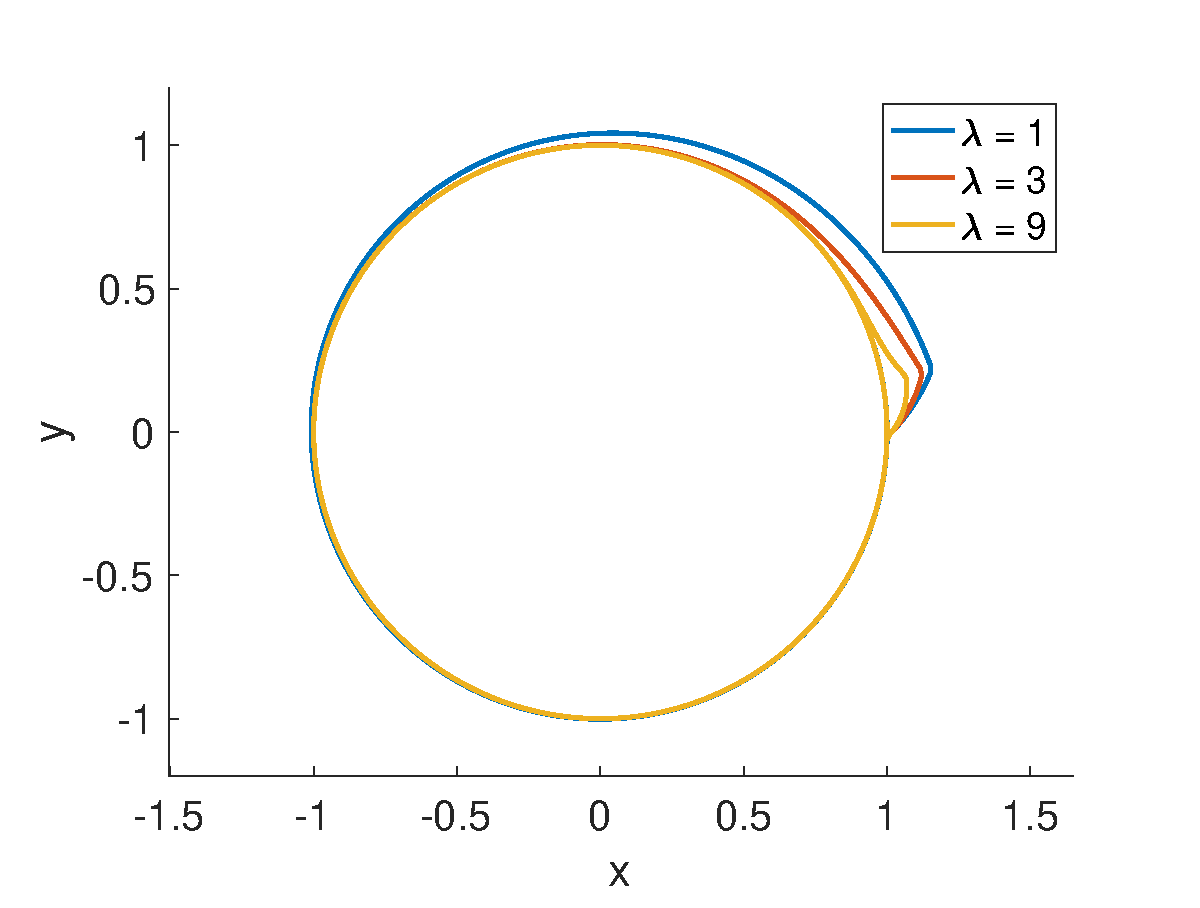
\includegraphics[width=1\linewidth]{Images/photo8_2.eps} 
  \end{minipage} 
  
  \caption{\textbf{Perturbed $\Lambda \Omega_{2}$ system within the same amplitude level set and recovery times.} Left: recovery times for different values of parameter $\lambda$ where $K_{a} = 1$. Right: perturbation shown on the $x-y$ parameter space for different values of parameter $\lambda$ where $K_{a}=1$ ($b=\lambda$). Parameter values: $a = 1$ and $\omega = 1$.}
  \label{photo8}
\end{figure}


\subsection{Total-degeneracy}
Throughout this work two attributes are considered to characterize oscillatory solutions: the amplitude and frequency. Thus, we say a level set is total-degenerated when both the amplitude and frequency are constant. If two or more systems (or networks) belong to the same total-degenerated level set, we say that systems (or networks) are total-degenerated.

As an example, total-degenerated level sets in $\Lambda \Omega_{2}$ systems preserving both the amplitude and frequency do exist and its analytical expression is given by Eqs. (\ref{e16}) and (\ref{e18}).

\section{Numerical Simulations}
All simulations have been performed and coded in MATLAB (Math Works, MA). The numerical simulations were computed by using the modified Euler method (Runge-Kutta, order two), with time steps within the $\Delta t =0.01$ and $\Delta t = 0.001$ range.
   % INCLUDE: introduction
\chapter{Level Sets Preservation in $\Lambda \Omega_{2}$ Networks}
\label{sec:results1}
In this section we study whether and under what condition the attribute level sets (LSs) for individual neurons are preserved in $\Lambda \Omega_{2}$ networks. Two $\Lambda \Omega_{2}$ networks with different degree of complexity are considered: the self-connected cell and the two-cell network.

A set of statements, aimed at capturing the main results, are presented in each section.

\section{The self-connected cell}
The set of equations describing the self-connected cell is given by

\begin{equation}
    \frac{dx}{dt} = \lambda x - \omega y - (bx + ay)(x^{2}+y^{2})+\alpha x
    \label{es11_1}
\end{equation}
\begin{equation}
    \frac{dy}{dt} = \omega x + \lambda y + (ax - by)(x^{2}+y^{2})
    \label{es11_2}
\end{equation}

where $\lambda$, $b$, $\omega$ and $a$ are the intrinsic parameters of the cell and $\alpha$ is the self-connectivity parameter.

A necessary condition for the preservation of individual LSs in $\Lambda \Omega_{2}$ networks is that the connectivity matrix has to be singular (see more details in Appendix \ref{sec:appendix}). Therefore, LSs in the self-connected cell will not be preserved.

\begin{Statement}
Attribute level sets are not preserved in the self-connected cell.
\end{Statement}

Fig. (\ref{photo9}) shows the effect of self-inhibition ($\alpha < 0$) and self-excitation ($\alpha > 0$) on different cells belonging to the same individual amplitude and frequency LS for representative parameter values. It is shown how amplitude and frequency are not constant along the individual LS. In particular, the effect of self-inhibition is a decrease in amplitude and frequency, while self-excitation increases both the amplitude and frequency. In both cases, the effect is greater specially for small values of parameter $\lambda$.

\begin{figure}[htb]
\centering
  \begin{minipage}{0.45\linewidth}
  \centering
    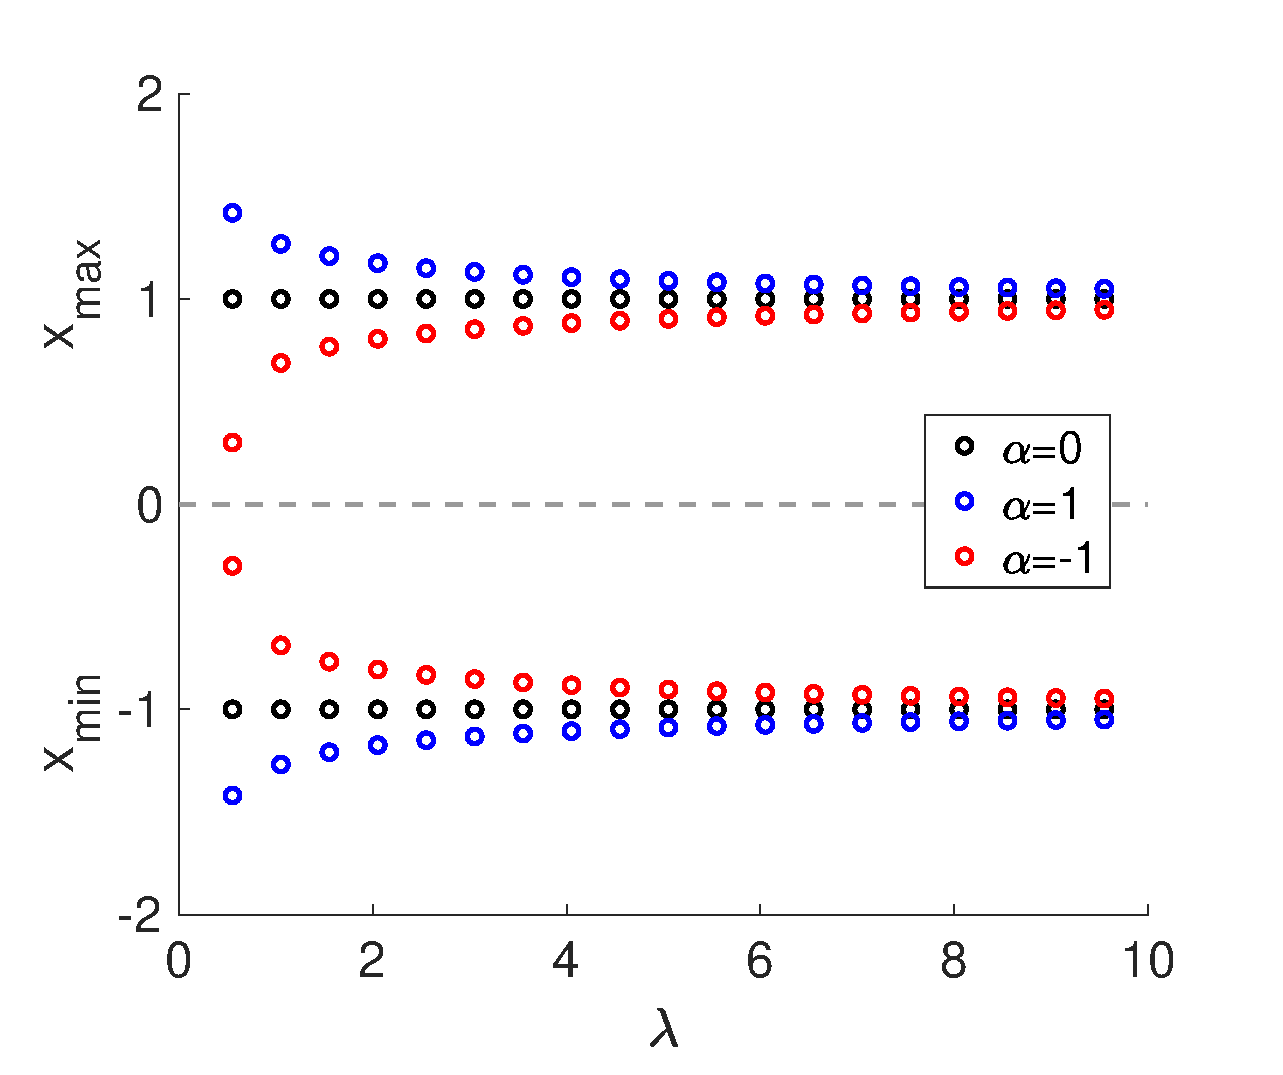
\includegraphics[width=1\linewidth]{Images/photo9_1.eps} 
  \end{minipage} 
  \begin{minipage}{0.45\linewidth}
  \centering
    \includegraphics[width=1\linewidth]{Images/photo9_2.eps} 
  \end{minipage} 
  
  \caption{\textbf{Individual attribute level sets are not preserved in the self-connected cell.} The individual cells belong to the same level set ($K_{a}=1$ and $K_{f}=2$). Left: amplitude envelope diagram as a function of $\lambda$ for representative values of self-connectivity parameter $\alpha$. Right: frequency diagram as a function of $\lambda$ for representative values of self-connectivity parameter $\alpha$. Parameter values: $a = 1$ and $\omega = 1$.}
  \label{photo9}
\end{figure}

\section{The Two-cell Network}
The set of equations describing the self-connected cell are given by

\begin{equation}
    \frac{dx_{1}}{dt} = \lambda_{1} x_{1} - \omega_{1} y_{1} - (b_{1}x_{1} + a_{1}y_{1})(x_{1}^{2}+y_{1}^{2}) + \alpha_{11}x_{1} + \alpha_{12}x_{2}
    \label{es121}
\end{equation}
\begin{equation}
  \frac{dy_{1}}{dt} = \omega_{1} x_{1} + \lambda_{1} y_{1} + (a_{1}x_{1} - b_{1}y_{1})(x_{1}^{2}+y_{1}^{2})
   \label{es122}
\end{equation}

\begin{equation}
    \frac{dx_{2}}{dt} = \lambda_{2} x_{2} - \omega_{2} y_{2} - (b_{2}x_{2} + a_{2}y_{2})(x_{2}^{2}+y_{2}^{2}) + \alpha_{21}x_{1} + \alpha_{22}x_{2}
     \label{es123}
\end{equation}
\begin{equation}
  \frac{dy_{2}}{dt} = \omega_{2} x_{2} + \lambda_{2} y_{2} + (a_{2}x_{2} - b_{2}y_{2})(x_{2}^{2}+y_{2}^{2})
   \label{es124}
\end{equation}

where $\lambda_{i}$, $b_{i}$, $\omega_{i}$ and $a_{i}$ ($i=1,2$) are the intrinsic parameters of the cells and $\{\alpha_{ij}\}_{i,j=1,2}$ is the connectivity matrix whose coefficients are the connectivity parameters.

We show that there exist conditions for individual LSs preservation in the two-cell network. In particular there exist 2-dimensional manifolds on connectivity parameter space which preserve individual LSs, provided individual cells belong to the same frequency LS.

Furthermore, analytical expression for these manifolds can be written down. We proceed as follows. Firstly, necessary and sufficient conditions for the existence of an individual limit circle in each cell are found. Under these conditions, each cell shows an individual limit circle for 2-dimensional manifolds on connectivity parameter space.

We notice that the existence of an individual limit circle in each cell is not sufficient for LSs preservation, since limit circles should be stable in order to show sustained oscillations. Then, we obtain (computationally) restricted 2-dimensional manifolds which preserve individual LSs. (see more details in Appendix \ref{sec:appendix}).

As a result, connectivity matrices preserving individual LSs can be found both in homogeneous and heterogeneous networks. In the following we summarize conditions for LSs preservation.

\begin{Statement} 
Individual cells must belong to the same frequency level set ($K_{f}$) in order to preserve attribute level sets. Therefore, heterogeneous networks in which cells belong to different frequency level sets do not preserve individual attribute level sets.
\end{Statement}

Taking into account the analytical expressions of amplitude and frequency LSs in $\Lambda \Omega_{2}$ systems, in the most general situation in which cells belong to different amplitude LSs ($K_{a1}$ and $K_{a2}$), intrinsic parameters $\omega_{1}$, $\omega_{2}$, $a_{1}$ and $a_{2}$ must verify the condition

\begin{equation}
    \omega_{1}+a_{1}K_{a1} = \omega_{2}+ a_{2}K_{a2}
    \label{es125}
\end{equation}

in order to belong to the same individual frequency LS.

\begin{Statement} 
Homogeneous and heterogeneous (cells belong to different individual amplitude level sets) two-cell networks preserve individual attribute level sets on 2-dimensional manifolds on connectivity parameter space. 
\end{Statement} 

We have found that there are two types of networks which preserve individual LSs, namely synchronized and non-synchronized networks. In synchronized networks, cells oscillate in phase ($\Delta \varphi = 0$), whereas in non-synchronized networks, cells oscillate in antiphase ($\Delta \varphi = \pm \pi$). Whether the network which preserve individual LSs is synchronized or not does depend on cross-connectivity parameters.

The following statement summarizes the possible networks according to the inhibitory (negative value) or excitatory (positive value) character of connectivity parameters. 

\begin{Statement} 
Mutually excitatory and inhibitory cross-connectivity under self-inhibition preserve level sets in the two-cell network. Mutually excitatory cross-connectivity leads to synchronized networks whereas mutually inhibitory cross-connectivity leads to non-synchronized networks.
\end{Statement} 

In order to compute closed matrix forms preserving individual LSs, we define the additional parameter

\begin{equation}
    \gamma = \frac{\bar{r_{1}}}{\bar{r_{2}}}
\end{equation}

where 

\begin{equation}
    \bar{r_{1}} = \sqrt{\frac{\lambda_{1}}{b_{1}}}  \hspace{0.5cm} \text{and} \hspace{0.5cm} \bar{r_{2}} = \sqrt{\frac{\lambda_{2}}{b_{2}}}
    \label{e28}
\end{equation}

are the amplitude value of cell-1 and cell-2 respectively. We note that parameter $\gamma$ has value one when cells are either identical (homogeneous networks) or belong to the same individual amplitude (and also frequency) LSs (type-\textrm{I} heterogeneous networks). In contrast, it has a different values when cells belong to different individual amplitude LSs (type-\textrm{II} heterogeneous networks).

\subsection{Non-Synchronized Networks Preserving Level Sets}
\begin{Statement} 
Connectivity matrices with the general form

\begin{equation}
   C_{\text{non-syn}} = 
    \begin{pmatrix}
        -\gamma^{-1}\alpha & -\alpha\\
        -\beta & -\gamma \beta
    \end{pmatrix}
    \text{ , } \hspace{0.5cm} \alpha, \beta \geq 0
    \label{e30}
\end{equation}

do preserve attribute LSs both in type-\textrm{I} heterogeneous (cells belong to the same amplitude and frequency LS) and type-\textrm{II} heterogeneous (cells belong to the different amplitude LSs) provided cells belong to the same frequency LS.
Furthermore networks are non-synchronized.
\end{Statement} 

Fig. (\ref{photo11}) shows voltage traces in a non-synchronized network preserving individual LSs. It is also shown how individual LSs of cell-1 are preserved in the network.

\begin{figure}[htb]
   \begin{minipage}{0.32\linewidth}
            \begin{center}
                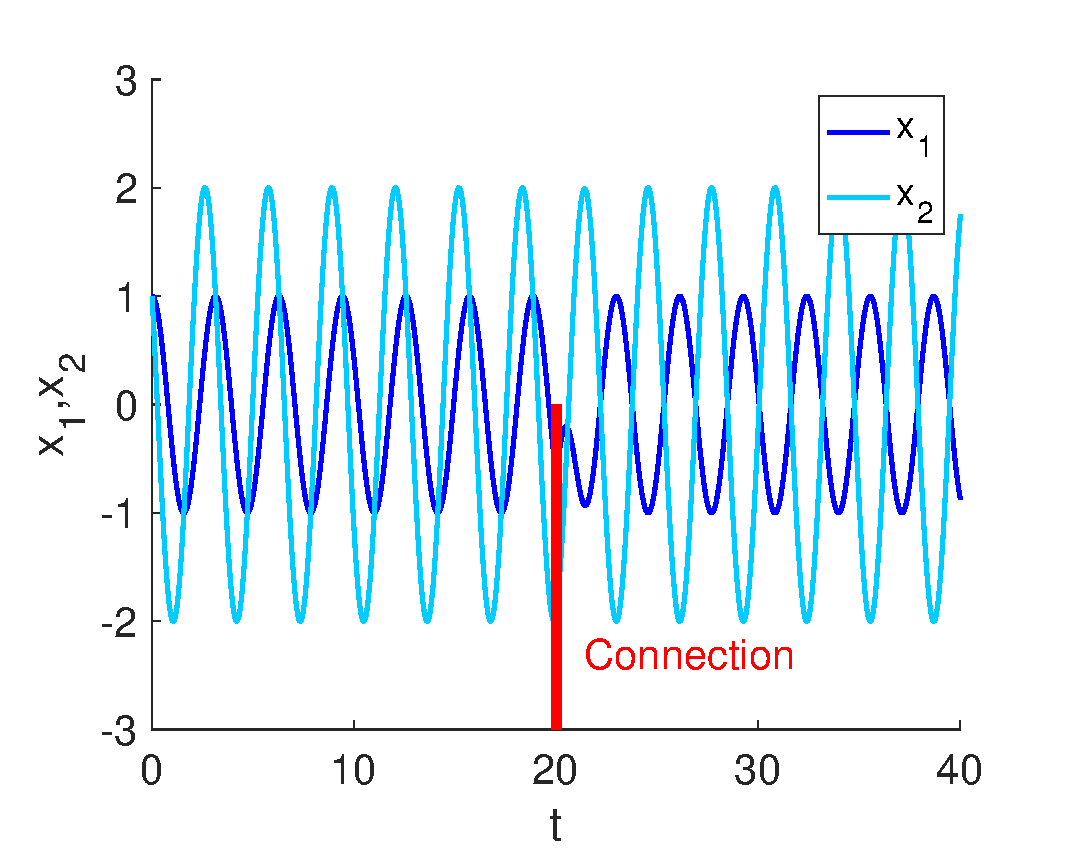
\includegraphics[width=1\linewidth]{Images/photo11_1.eps}
            \end{center}
        \end{minipage} 
        \begin{minipage}{0.32\linewidth}
            \begin{center}
                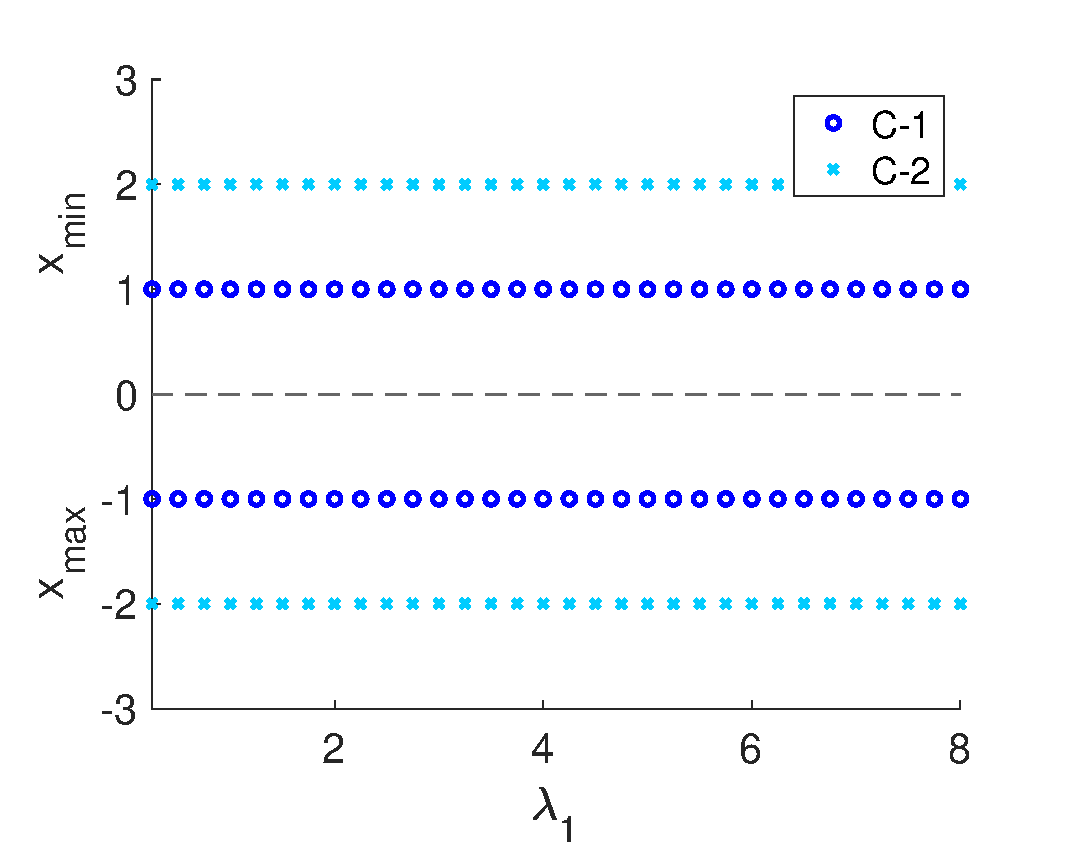
\includegraphics[width=1\linewidth]{Images/photo10_2.eps}
            \end{center}
        \end{minipage} 
    \begin{minipage}{0.32\linewidth}
        \begin{center}
            \includegraphics[width=1\linewidth]{Images/photo10_3.eps}
        \end{center}
    \end{minipage} 
  \caption{\textbf{Non-Synchronized network preserving individual attribute level sets.} Left: voltage traces $x_{1}$ and $x_{2}$ before and after the connection. Vertical Red line indicates the time at which cells form the network. Middle: amplitude envelope diagram for values $(\lambda_{1},b_{1})$ belonging to the same individual amplitude level set ($K_{a,1}=1$). Left: frequency diagram for values $(\lambda_{1},b_{1})$ belonging to the same individual amplitude level set ($K_{a,1}=1$). Parameter values: $a_{1} = 1$, $\omega_{1} = 1$, $a_{2}=1/4$, $\omega_{2} = 1$, $\gamma = 1/2$, $\alpha = 1$ and $\beta=1$.}
  \label{photo11}
\end{figure}

\subsection{Synchronized Networks Preserving Level Sets}
\begin{Statement} 
Connectivity matrices with the general form
\begin{equation}
   C_{\text{syn}} = 
    \begin{pmatrix}
        -\gamma^{-1}\alpha & \alpha\\
        \beta & -\gamma \beta
    \end{pmatrix}
    \text{ , } \hspace{0.5cm} \alpha, \beta \geq 0
    \label{e29}
\end{equation}
do preserve attribute level set both in type-\textrm{I} heterogeneous (cells belong to the same amplitude and frequency LS) and type-\textrm{II} heterogeneous (cells belong to the different amplitude LSs) provided cells belong to the same frequency level set . Furthermore networks are synchronized.
\end{Statement} 

Fig. (\ref{photo10}) shows voltage traces in a synchronized network preserving individual attributes LSs. It is also shown how individual LSs of cell-1 are preserved in the network.

 \begin{figure}[htb]
        \begin{minipage}{0.32\linewidth}
            \begin{center}
                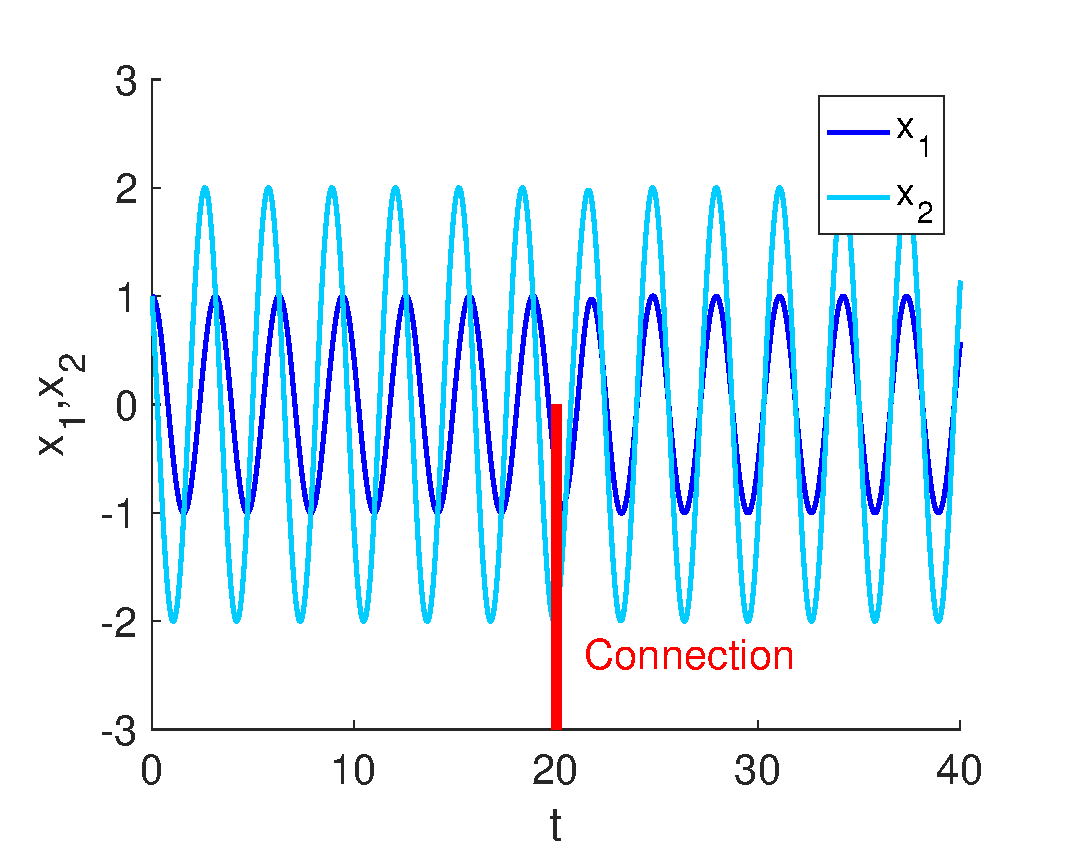
\includegraphics[width=1\linewidth]{Images/photo10_1.eps}
            \end{center}
        \end{minipage} 
        \begin{minipage}{0.32\linewidth}
            \begin{center}
                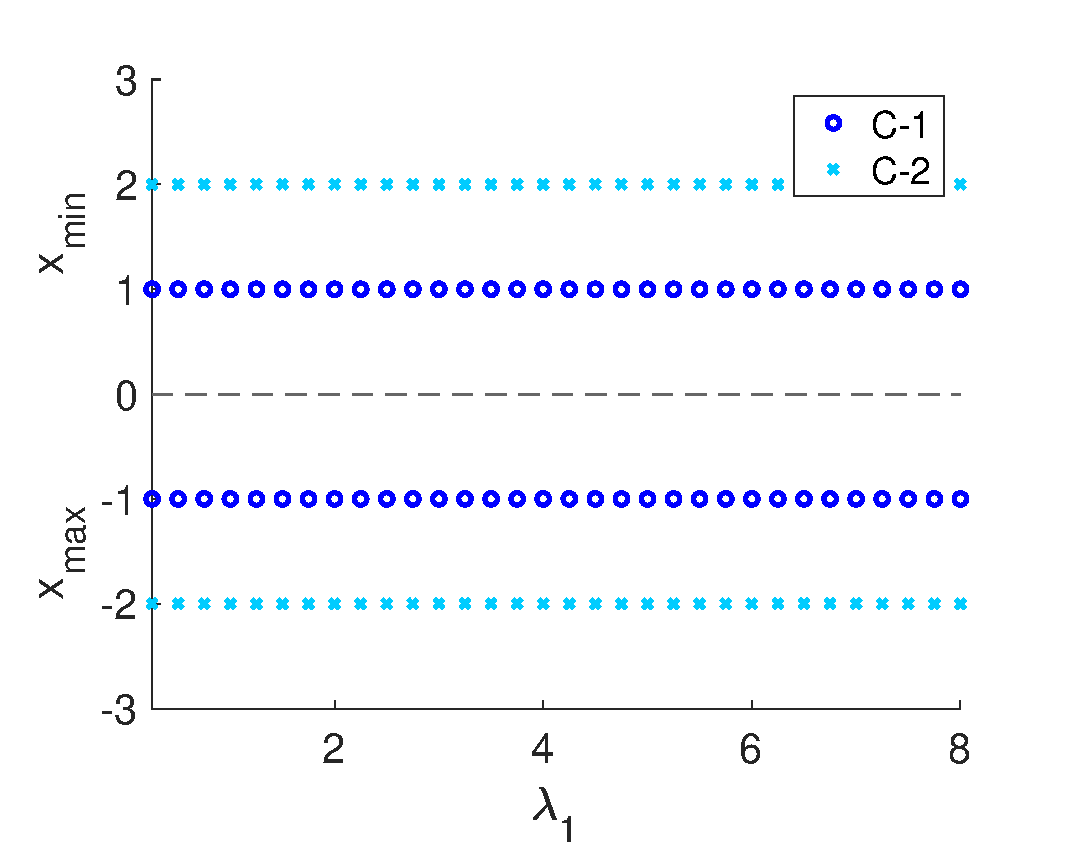
\includegraphics[width=1\linewidth]{Images/photo10_2.eps}
            \end{center}
        \end{minipage} 
    \begin{minipage}{0.32\linewidth}
        \begin{center}
            \includegraphics[width=1\linewidth]{Images/photo10_3.eps}
        \end{center}
    \end{minipage} 
  
  \caption{\textbf{Synchronized network preserving individual attribute level sets.} Left: voltage traces $x_{1}$ and $x_{2}$ before and after the connection. Vertical Red line indicates the time at which cells form the network. Middle: amplitude envelope diagram for values $(\lambda_{1},b_{1})$ belonging to the same individual amplitude level set ($K_{a,1}=1$). Left: frequency diagram for values $(\lambda_{1},b_{1})$ belonging to the same individual amplitude level set ($K_{a,1}=1$). Parameter values: $a_{1} = 1$, $\omega_{1} = 1$, $a_{2}=1/4$, $\omega_{2} = 1$, $\gamma = 1/2$, $\alpha = 1$ and $\beta=1$.}
  \label{photo10}
\end{figure}

\subsubsection{Gap-Junctions: Synchronized Electrical Network Preserving Level Sets}

We highlight synchronized type-I heterogeneous networks, which preserve individual LSs. In this case, matrices preserving individual LSs has the general form

\begin{equation}
   C_{\text{gap-juntion}} = 
    \begin{pmatrix}
        -\alpha & \alpha\\
        \beta & -\beta
    \end{pmatrix}
    \text{ , } \hspace{0.5cm} \alpha, \beta \geq 0
\end{equation}

This kind of connectivity would corresponds to the case where cells are coupled through electrical synapses or gap junctions. In realistic neuron network models, electrical synapses would produce a synaptic current proportional to the difference between the pre- and post-synpatic membrane potentials, \cite{book1}.

\begin{Statement} 
Gap juntions preserve level sets in type-\textrm{I} heterogeneous networks where cells belong to the same amplitude and frequency level set. However, gap-junctions do not preserve individual level sets in type-\textrm{II} heterogeneous networks.
\end{Statement}
   % INCLUDE: introduction
\chapter{Newly Emerged Network Level Sets}
\label{sec:results2}
In this section we study the newly emerged network LSs when individual LSs are not preserved in the network.

In chapter \ref{sec:results1} we focus on conditions for individual LSs preservation in the self-connected cell and the two-cell network. When those conditions are not guaranteed, new network LSs emerge. The goal of this section is to characterize them for different types of networks: homogeneous networks (identical cells), type-\textrm{I} heterogeneous networks (cells belong to the same amplitude and frequency  LS) and type-\textrm{II} heterogeneous networks (cells belong to different frequency and/or amplitude LSs).

We begin characterizing the new network LSs on the connectivity parameter space focusing on connectivity parameter dependencies for the preservation of network attributes. We also investigate the intrinsic parameter space of a single cell and combined parameter spaces involving both connectivity and intrinsic parameters.

\section{The self-connected cell}
As it was shown in chapter \ref{sec:results1}, self-connected cells do not preserve individual LSs. Therefore all network LSs found will be characteristic of the self-connected cell.

Firstly, we study separately the $\lambda-b$ and $\omega-a$ parameter spaces for different values of self-connectivity parameter $\alpha$. Afterwards, we characterize total-generated LSs on the whole intrinsic parameter space and describe parameter dependencies needed to maintain network attributes constant on parameter space.

\subsection{The $\lambda-\alpha$ parameter space}
Individual amplitude LSs are defined in the $\lambda-b$ parameter space and they are total-degenerated since the frequency is also constant along them. To begin with, we consider the $\lambda-b$ parameter space to compare LSs on this parameter space between the self-connected cell and the individual cell.

\begin{Statement}
Amplitude level sets on the $\lambda-b$ parameter space in the self-connected cell are not total-degenerated. The network frequency is not preserved along amplitude level sets on the $\lambda-b$ parameter space.
\end{Statement}

Fig. (\ref{photo12}) shows a representative amplitude LS ($A_{\text{Net}} = 1$) on the $\lambda-\alpha-b$ parameter space. It is also shown the network frequency for each point on the amplitude LS. In particular, when the connectivity parameter $\alpha$ is fixed, it is shown the change in frequency along the amplitude LSs ($A_{\text{Net}} = 1$) on the $\lambda-b$ parameter space.

\begin{figure}[h]
\centering
  \begin{minipage}{0.45\linewidth}
  \centering
    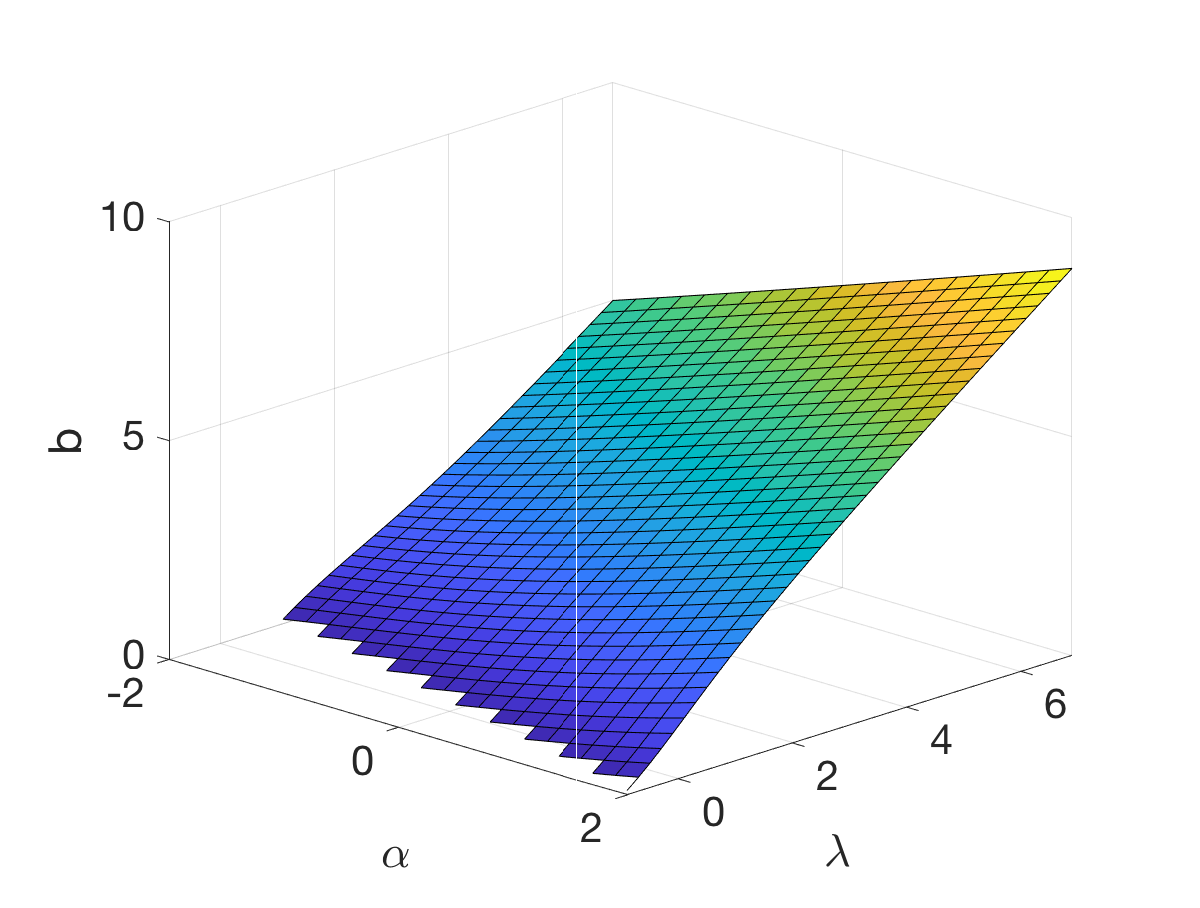
\includegraphics[width=1\linewidth]{Images/photo12_1.eps} 
  \end{minipage} 
  \begin{minipage}{0.45\linewidth}
  \centering
    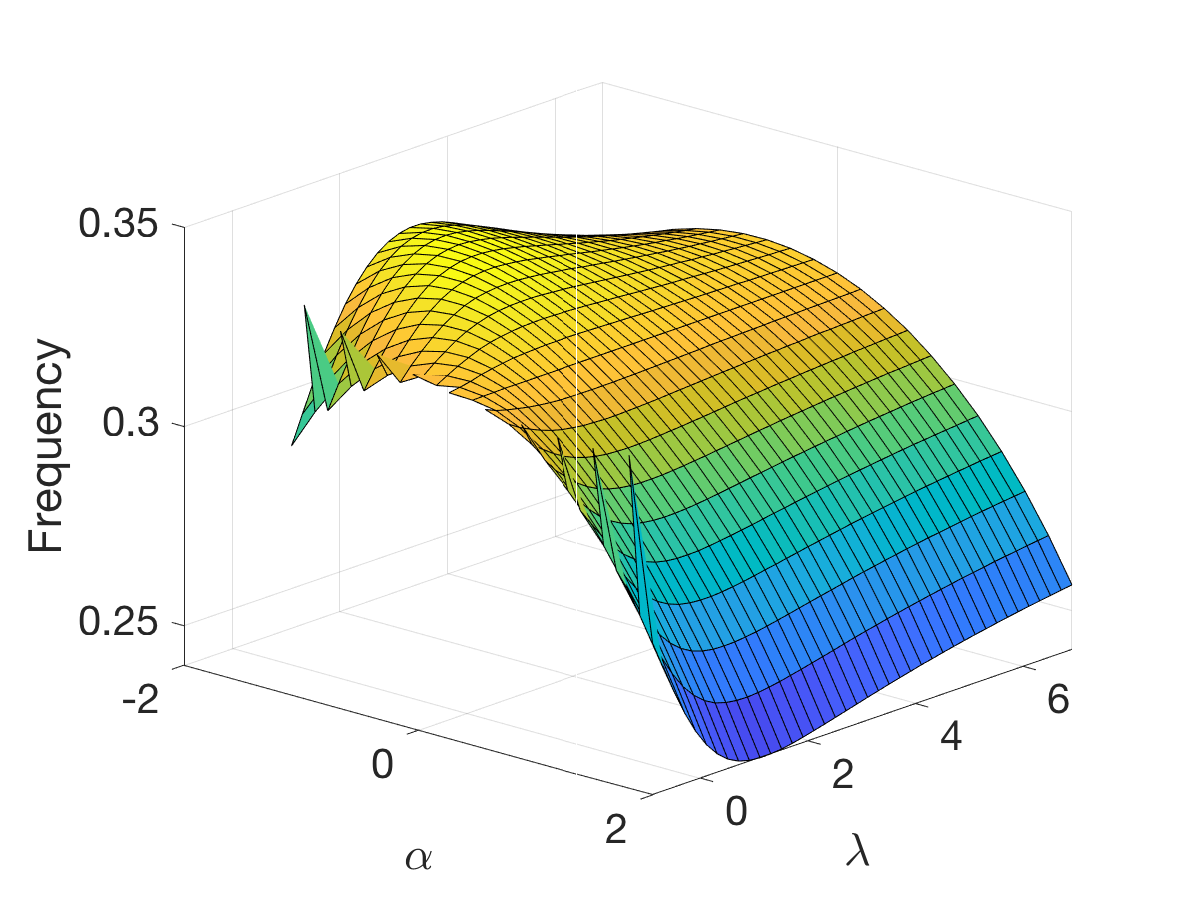
\includegraphics[width=1\linewidth]{Images/photo12_2.eps} 
  \end{minipage} 
 
  \caption{\textbf{Network frequency is not constant on amplitude LSs on the $\lambda-\alpha-b$ parameter space.} Left: amplitude LS ($A_{Net} = 1$) on the $\lambda-\alpha-b$ parameter space. Right: network frequency for each point on the amplitude LS. Parameter values: $a = 1$ and $\omega = 1$.}
  \label{photo12}
\end{figure}

We note that 1-dimensional total-degenerated LSs could be found in the $\lambda-\alpha-b$ parameter space following trajectories within the amplitude LS which preserve the network frequency.

\subsection{The $\omega-a$ parameter space}
If the $\omega-a$ parameter space is considered, similar results are obtained. More specifically, individual total-degenerated LSs on the $\omega-a$ parameter space are no longer total-degenerated in the self-connected cell due to the fact that frequency LSs do not preserve the network amplitude.

\begin{Statement}
Frequency level sets on the $\omega-a$ parameter space in the self-connected cell are not total-degenerated. The network amplitude is not preserved along frequency level sets on the $\omega-a$ parameter space.
\end{Statement}

Fig. (\ref{photo13}) shows a representative frequency LS ($f_{\text{Net}} = \pi^{-1}$) on the $\omega-\alpha-a$ parameter space. It is also shown the network amplitude for each point on the amplitude LS. 

\begin{figure}[h]
\centering
  \begin{minipage}{0.45\linewidth}
  \centering
    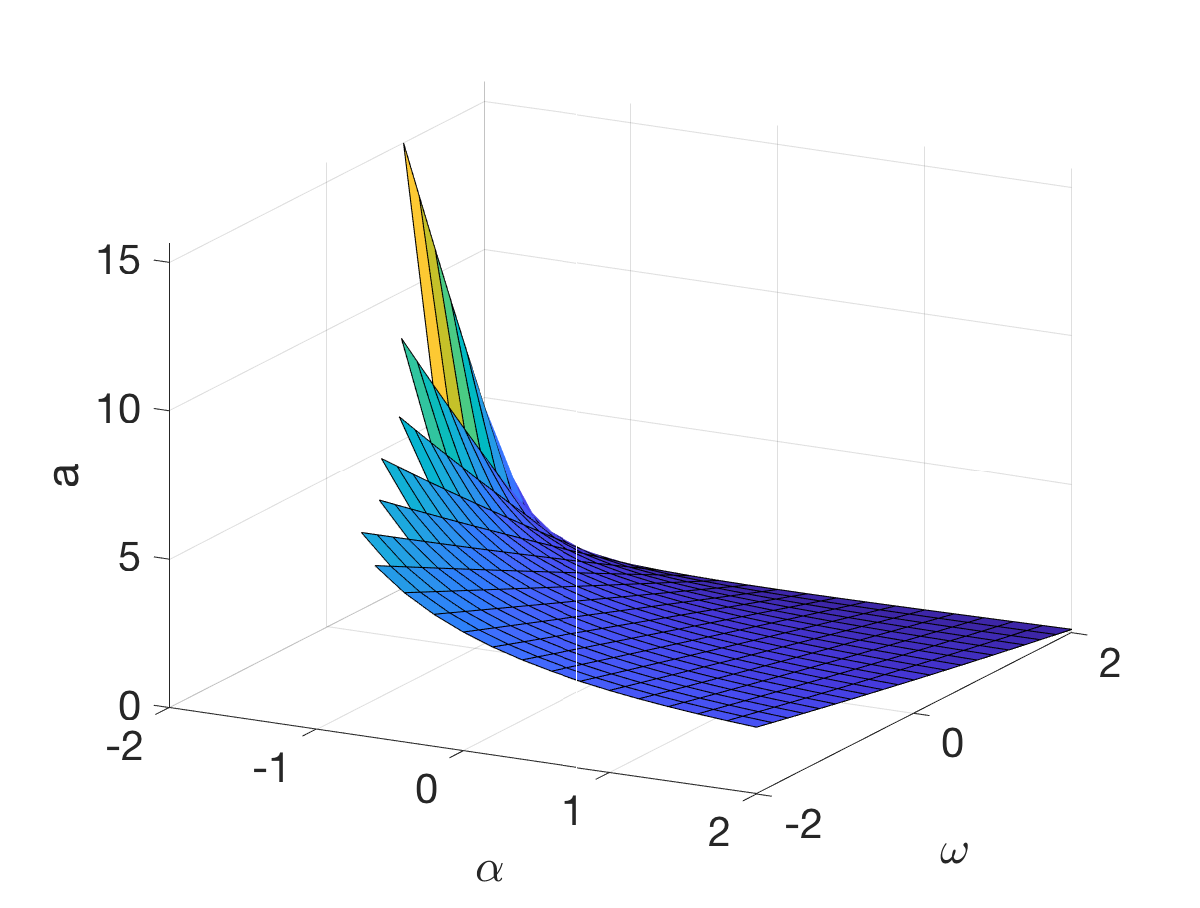
\includegraphics[width=1\linewidth]{Images/photo13_1.eps} 
  \end{minipage} 
  \begin{minipage}{0.45\linewidth}
  \centering
    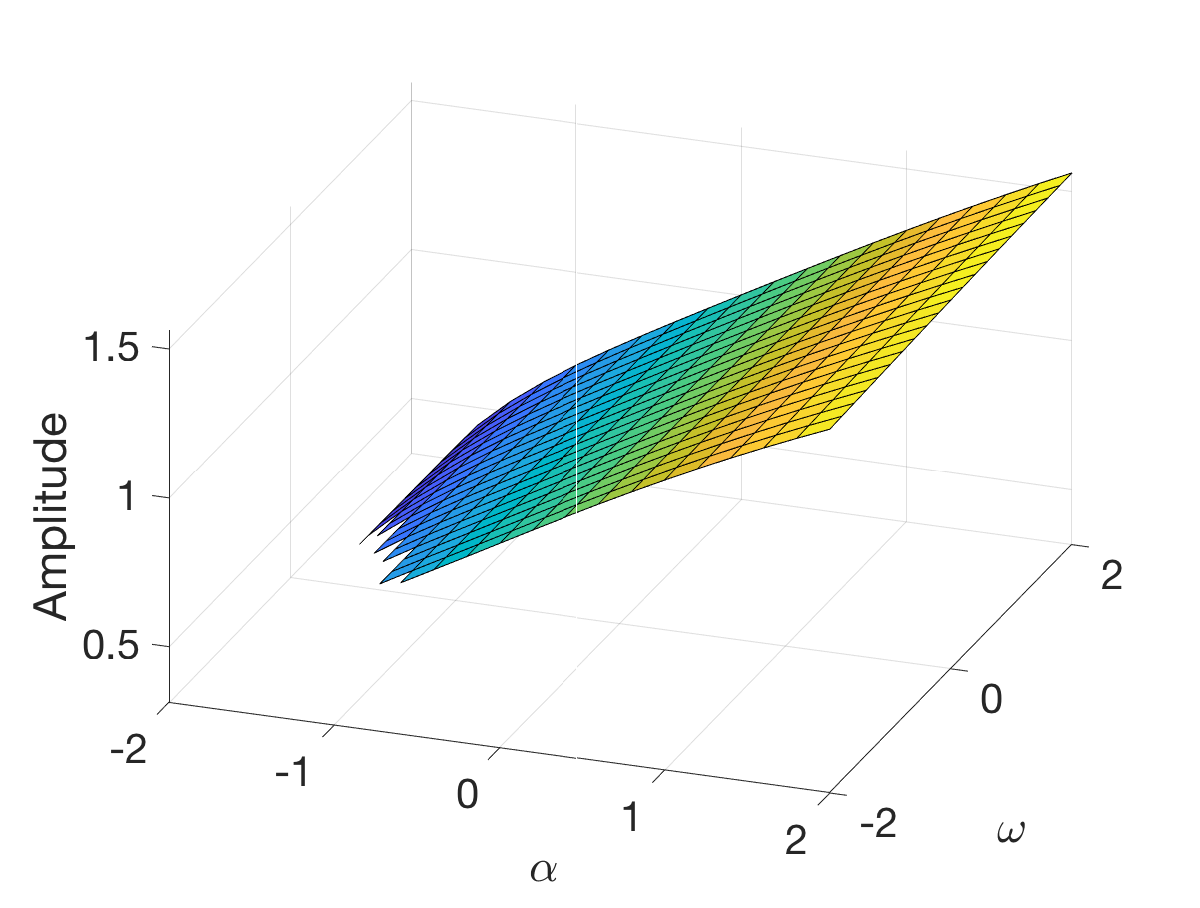
\includegraphics[width=1\linewidth]{Images/photo13_2.eps} 
  \end{minipage} 
 
 \caption{\textbf{Network amplitude is not constant on frequency LSs on the $\omega-\alpha-a$ parameter space.} Left: frequency LS ($A_{Net} = \pi^{-1}$) on the $\omega-\alpha-a$ parameter space. Right: network amplitude for each point on the frequency LS. Parameter values: $\lambda= 1$ and $b = 1$.}
  \label{photo13}
\end{figure}

We note that if the self-connectivity parameter $\alpha$ is fixed, amplitude does not remain constant on frequency LSs in the $\omega-a$ parameter space. Although it is indeed not constant, the variation in the network amplitude is quite small (not easily deduced from Fig. (\ref{photo13})-Right). As a consequence, the network amplitude does depend on parameters $\omega$ and $a$ in the self-connected cell, which is a new feature characterizing self-connected cells.

Furthermore, 1-dimensional total-degenerated LSs could be found in the $\omega-\alpha-a$ parameter space following trajectories within the frequency LS which preserve the network amplitude.

As a global picture, Fig. (\ref{photo14}) shows amplitude and frequency LSs in the form of colored heat graphs, where each point represents a single self-connected cell with a specific combination of parameters $\lambda$ and $b$ (top) and $\omega$ and $a$ (bottom) whose network amplitude (left) and frequency (right) corresponds with the value indicated on the color bar. LSs corresponds to the curves joining points with the same attribute value.

\begin{figure}[h]
\centering
\begin{minipage}{0.45\linewidth}
  \begin{center}
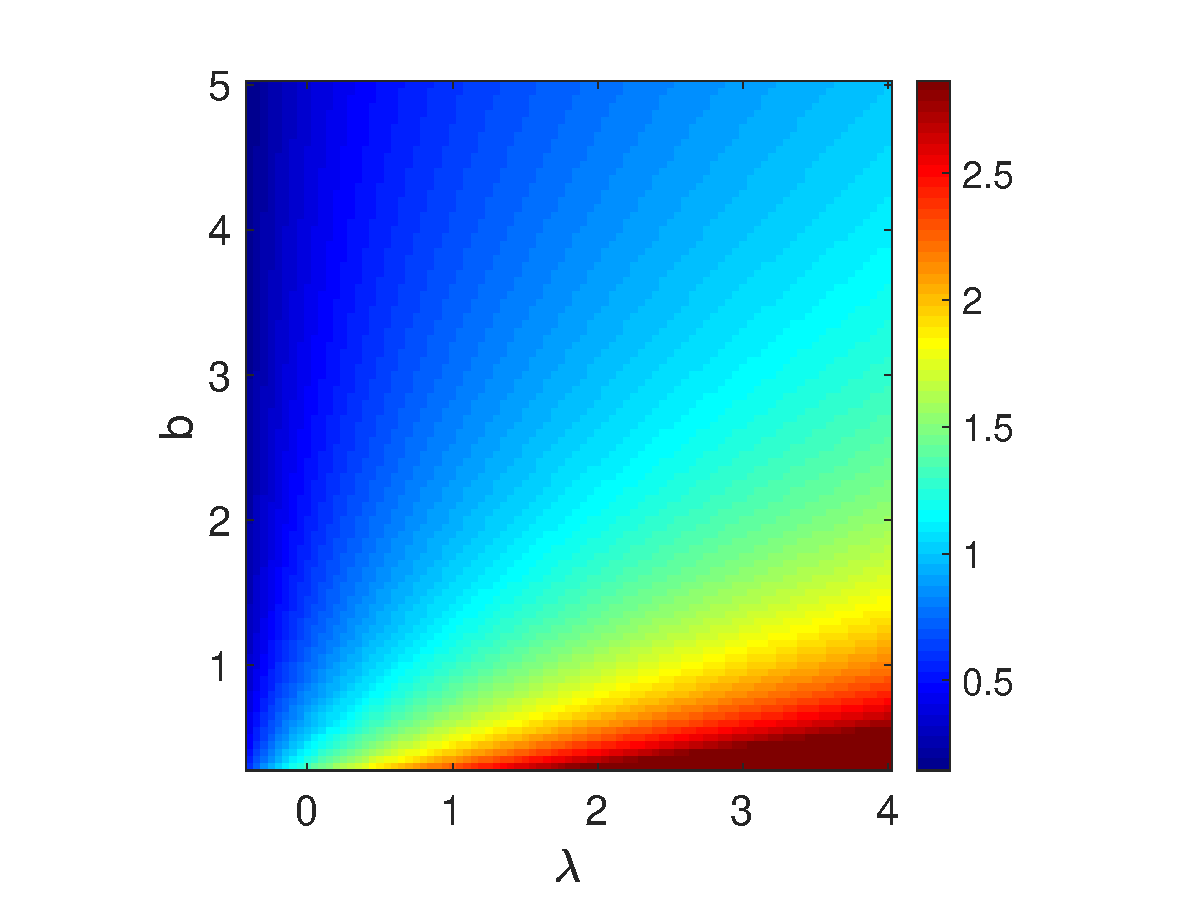
\includegraphics[width=1\linewidth]{Images/photo14_1.eps}
\end{center}
  \end{minipage} 
  \begin{minipage}{0.45\linewidth}
  \begin{center}
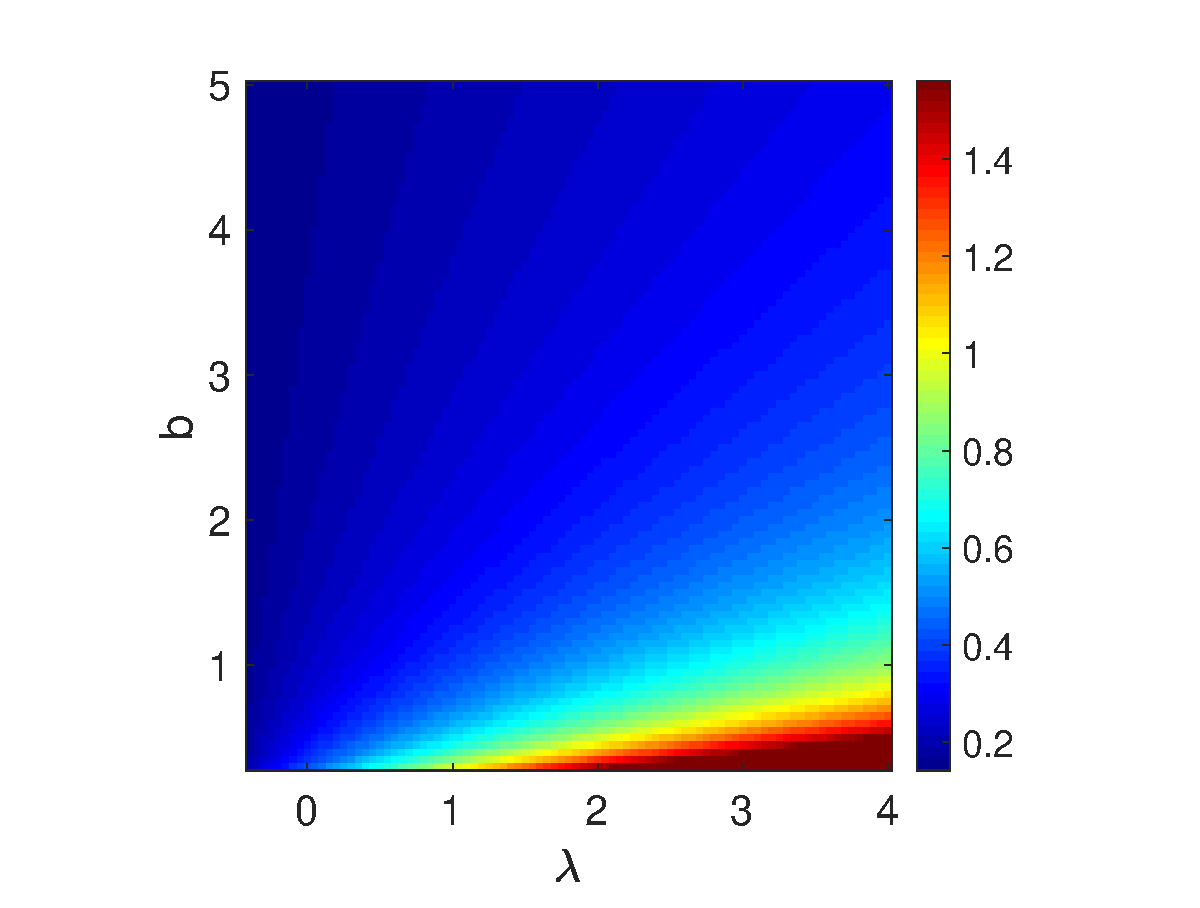
\includegraphics[width=1\linewidth]{Images/photo14_2.eps}
\end{center}

  \end{minipage} 
  
  \begin{minipage}{0.45\linewidth}
  \begin{center}
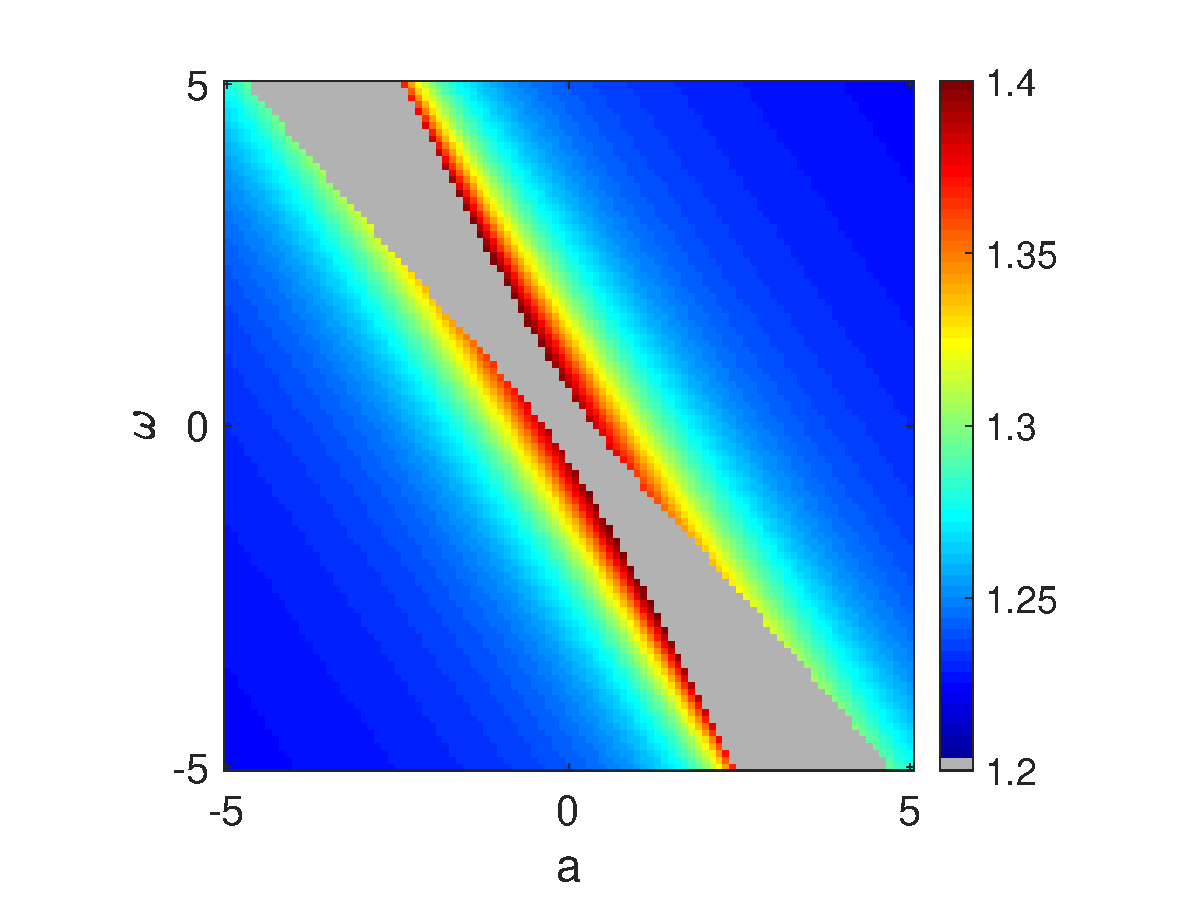
\includegraphics[width=1\linewidth]{Images/photo14_3.eps}
\end{center}
  \end{minipage} 
  \begin{minipage}{0.45\linewidth}
  \begin{center}
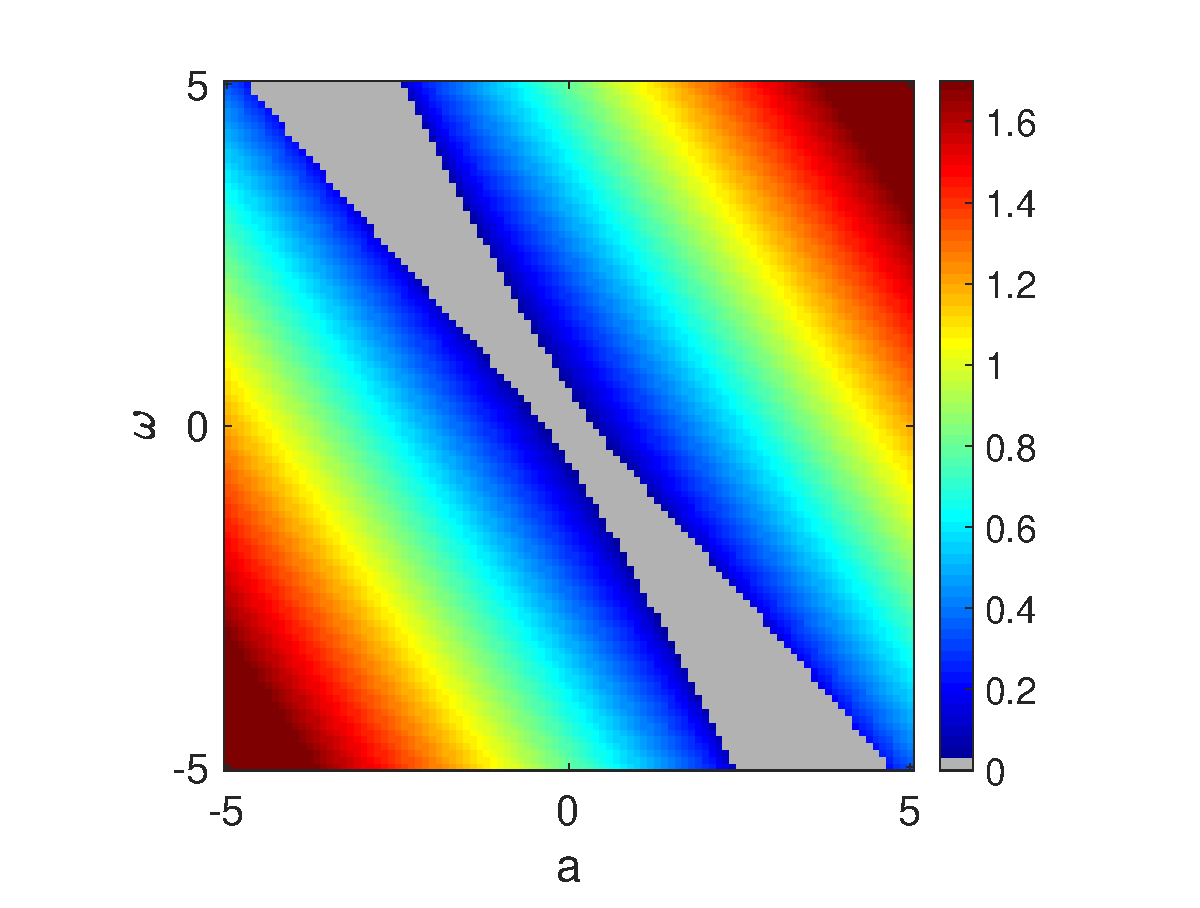
\includegraphics[width=1\linewidth]{Images/photo14_4.eps}
\end{center}

  \end{minipage} 
  
  \caption{\textbf{Amplitude and frequency LSs on the $\lambda-b$ and $\omega-a$ parameter spaces in the self-connected cell.} Top: amplitude (left) and frequency (right) LSs on the $\lambda-b$ parameter space. Bottom: amplitude (left) and frequency (right) LSs on the $\omega-a$ parameter space. The grey region corresponds to points in the parameter space for which there are not sustained oscillations. Parameter values. Top: $a = 1$, $\omega = 1$ and $\alpha = 1$. Bottom $\lambda = 1$, $b=1$ and $\alpha = 1$.}
  \label{photo14}
\end{figure}

\subsection{The whole intrinsic parameter space}
Once characterized amplitude and frequency LSs on the $\lambda-b$ and $\omega-a$ parameter spaces separately, we extent the parameter space in order to characterize total-degenerated LSs on the whole intrinsic parameter space.

We found 2-dimensional manifolds on the intrinsic parameter space preserving the network amplitude and frequency.

\begin{Statement}
The self-connected cell show 2-dimensional total-degenerated level sets on the intrinsic parameter space (the $a-b-\lambda-\omega$ parameter space).
\label{s10}
\end{Statement}

Computationally, we have found that in order to compute most general total-degenerated LSs, compensating parameters must be chosen appropriately. One of them must be either parameter $\lambda$ or $b$, whereas the other must be either parameter $\omega$ or $a$. This ensures that the most general total-degenerated LSs can be found.
 
Fig. (\ref{photo15}) shows an example of a total-degenerated LS ($A_{\text{Net}} = 1 $ and $f_{\text{Net}} = \pi^{-1}$) on the $a-b-\lambda-\omega$ parameter space in the self-connected cell for representative parameter values. In this case, we choose compensating parameters to be parameters $a$ and $b$. It shows in the form of colored heat graphs, compensated parameters $\lambda$ (left) and $\omega$ (right) for each pair of compensating parameters $a$ and $b$. Each point on the 2-dimensional manifold represents a self-connected cell with the same network amplitude ($A_{\text{Net}} = 1 $) and frequency ($f_{\text{Net}} = \pi^{-1}$).

  \begin{figure}[h]
  \centering
        \begin{minipage}{0.4\linewidth}
            \begin{center}
                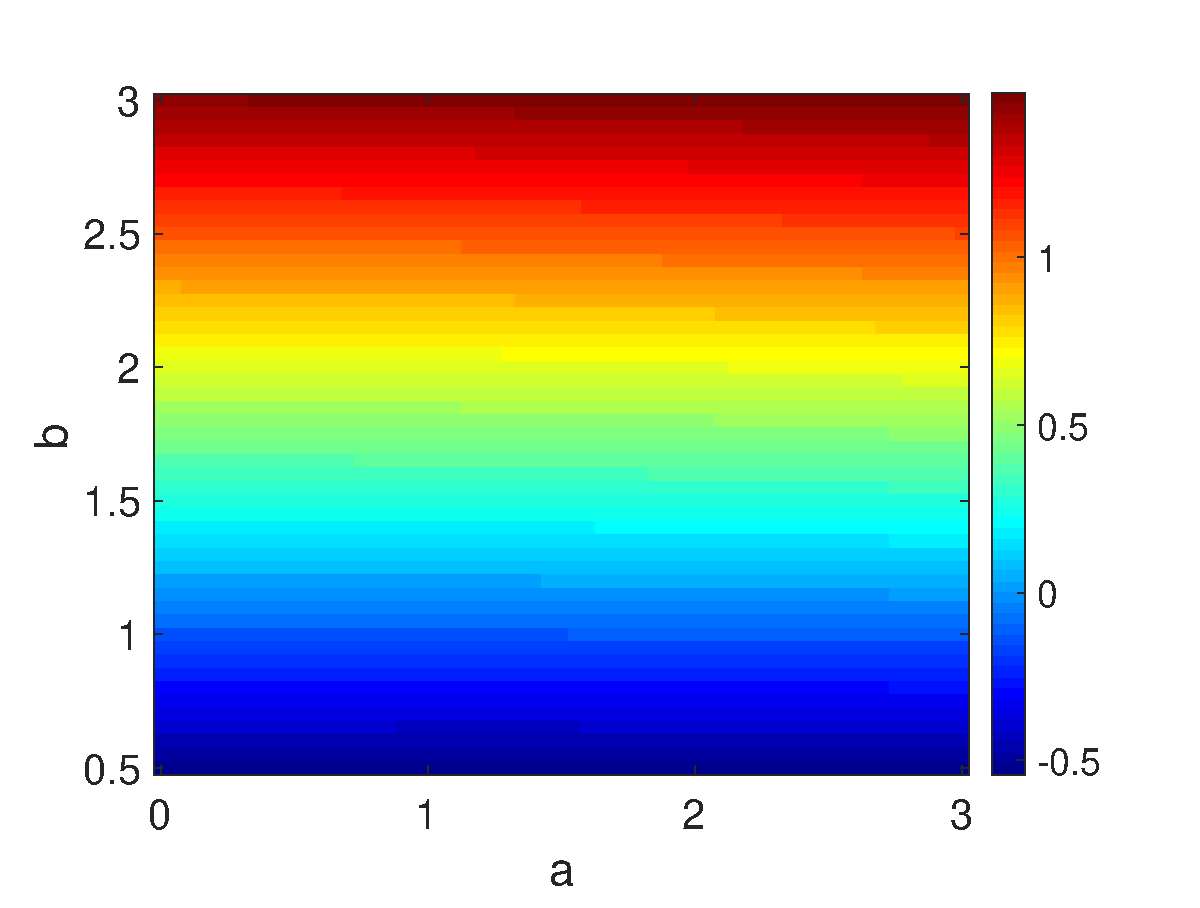
\includegraphics[width=1\linewidth]{Images/photo15_1.eps}
            \end{center}
        \end{minipage} 
        \begin{minipage}{0.4\linewidth}
            \begin{center}
                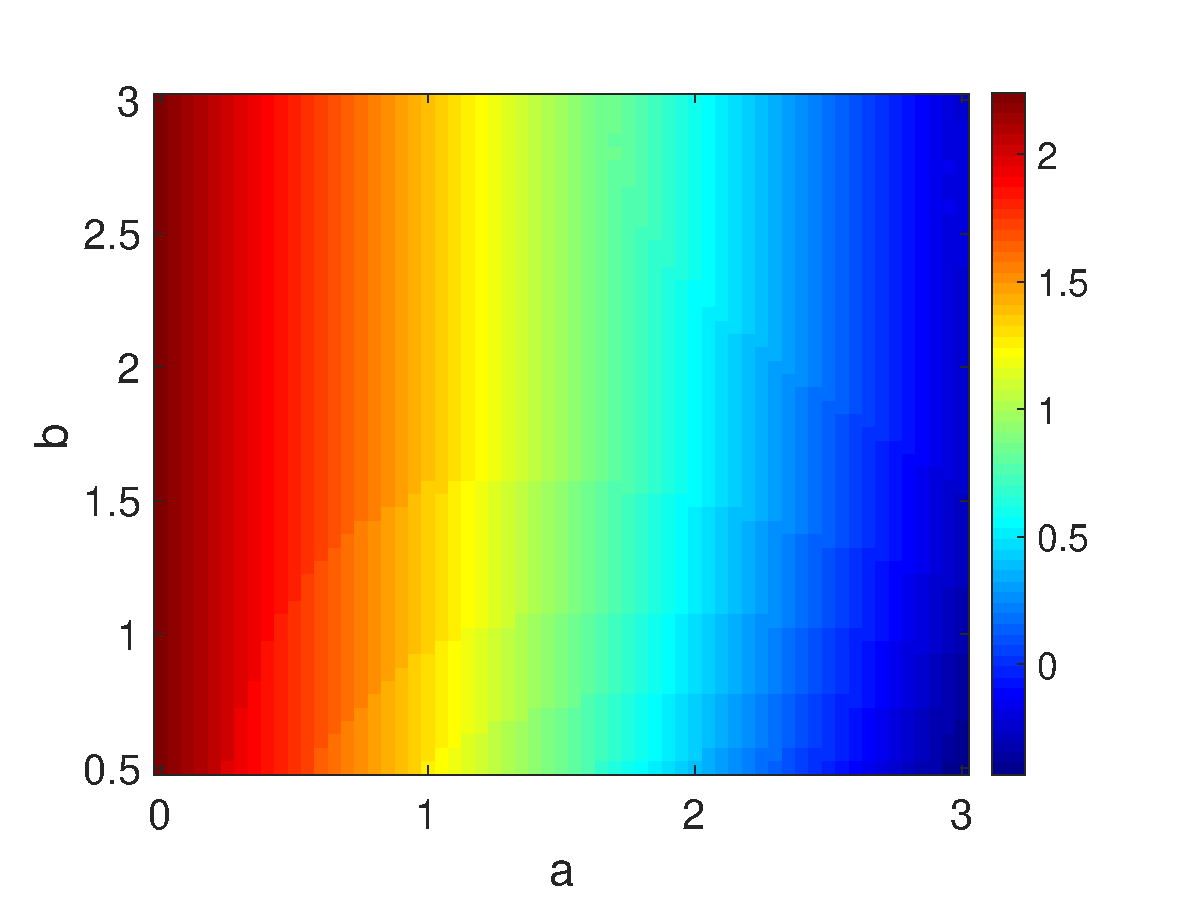
\includegraphics[width=1\linewidth]{Images/photo15_2.eps}
            \end{center}
        \end{minipage} 
  
  \caption{\textbf{Total-degenerated LS on the whole intrinsic parameter space in the self-connected cell.} The cell oscillates with amplitude $A_{\text{Net}} = 1$ and frequency $f_{\text{Net}} = \pi^{-1}$. For each pair of parameters $a$ and $b$, there are the values of parameters $\lambda$ (Left) and $\omega$ (Right), such as the amplitude and the frequency of the self-connected cell is preserved. Parameter values: $\alpha = 2$.}
  \label{photo15}
\end{figure}

Although individual total-degenerated LSs are also 2-dimensional manifolds on parameter space, there are some differences regarding compensatory functions, between total-degenerated LSs in the individual and the self-connected cell.

On the one hand, compensatory functions for total-degenerated LSs in the individual cell only depend on one compensating parameter. More specifically, parameter $b$ compensates parameter $\lambda$, while parameter $a$ compensates parameter $\omega$. 

On the other hand, compensatory functions in the self-connected cell depend on both compensating parameters, and therefore, each parameter ($\lambda$ and $\omega$) is compensated by both compensating parameters ($a$ and $b$).

In particular, Fig. (\ref{photo15}) shows the dependence on compensating parameters of compensatory functions on a representative total-degenerated LS ($A_{Net}=1$ and $f_{Net} = \pi^{-1}$). In order to gain insight into these compensatory dependencies between intrinsic parameters, we fix one compensating parameter and compute exact total-degenerated LS on the remaining 3-dimensional parameter space.

Fig. (\ref{photo16})-Left shows a representative total-degenerated LS on the $a-\lambda-\omega$ parameter space in which compensating parameter $b$ has been fixed. Conversely, Fig. (\ref{photo16})-Right shows a representative total-degenerated LS on the $b-\lambda-\omega$ parameter space in which compensating parameter $a$ has been fixed. 

  \begin{figure}[h]
  \centering
        \begin{minipage}{0.45\linewidth}
            \begin{center}
                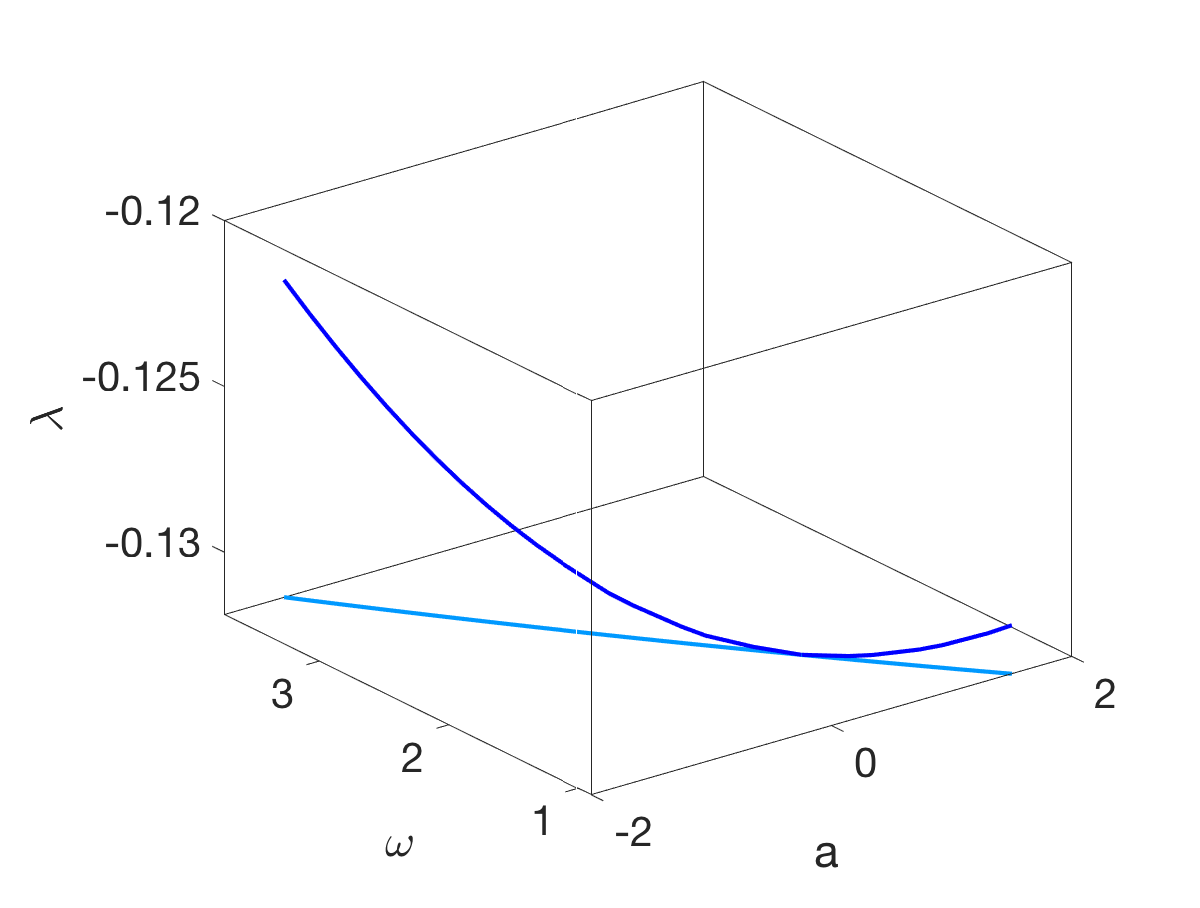
\includegraphics[width=1\linewidth]{Images/photo16_1.eps}
            \end{center}
        \end{minipage} 
        \begin{minipage}{0.45\linewidth}
            \begin{center}
                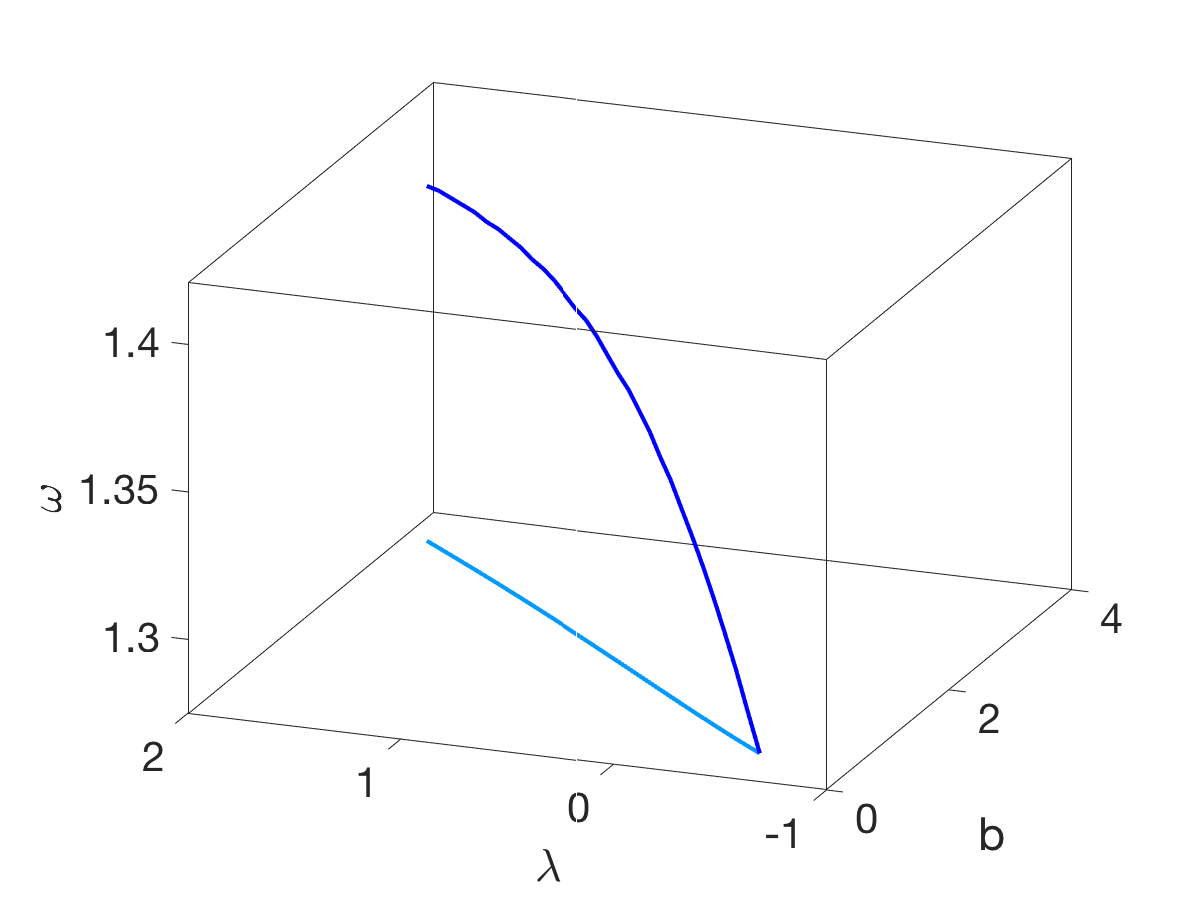
\includegraphics[width=1\linewidth]{Images/photo16_2.eps}
            \end{center}
        \end{minipage} 
  
  \caption{\textbf{Total-degenerated levels set on 3-dimensional intrinsic parameter spaces.} Left: compensating parameter $b$ is fixed and the 1-dimensional total-degenerated LS on the $a-\lambda-\omega$ parameter space is shown. Parameter values: $b=1$ and $\alpha=2$. Right: Compensating parameter $a$ is fixed and the 1-dimensional total-degenerated LS $a-\lambda-\omega$ parameter space is shown. Parameter values: $a=1$ and $\alpha=2$. Dark blue: 1-dimensional total-degenerated LSs. Light blue: LSs projections into $\omega-a$ (Left) and $\lambda-b$ (Right) parameter spaces.}
  \label{photo16}
\end{figure}

We see a monotonic and almost linear compensating dependencies between parameters $a-\omega$ and $b-\lambda$ in each case, which is clearly shown on the projection of each LS onto the $a-\omega$ or $b-\lambda$ parameter space (light blue lines in Fig. (\ref{photo16})). We note that the same type of compensating dependencies is observed in the individual cell.

In addition, parameters $\lambda$ (Fig. (\ref{photo16})-Left) and $\omega$ (Fig. (\ref{photo16})-Right) must be compensated in order to preserve network attributes. However, the strength of these new compensatory dependencies are weaker, since these additional compensated parameters are slightly changed, in comparison with parameters $\omega$ and $\lambda$, respectively.

The main reason of these parameter dependencies is the fact that the network frequency is mainly determined by parameters $\omega$ and $a$ and the network amplitude by parameters $\lambda$ and $b$. Therefore, although the self connection introduces new dependencies on parameters spaces $\lambda-b$ and $\omega-a$, these are weaker than the original ones.

\section{Homogeneous Two-Cell Networks}
In homogeneous two-cell networks, cells are identical and, therefore, they have same intrinsic parameters

\begin{equation}
   \lambda_{1}=\lambda_{2}(=\lambda) \text{,} \hspace{0.5cm} b_{1} = b_{2}(=b) \text{,} \hspace{0.5cm} a_{1}=a_{2}(=a) \hspace{0.5cm} \text{ and } \hspace{0.5cm} \omega_{1} = \omega_{2}(=\omega)
\end{equation}

\subsection{Symmetrical Networks}
\subsubsection{The connectivity parameter space}
In first place, we characterize amplitude and frequency LSs on the 4-dimensional connectivity parameter space in symmetrical homogeneous networks, where cells have the same network amplitude ($A_{\text{Net}}$) and frequency ($f_{\text{Net}}$) value.

Fig. (\ref{photo17}) shows an example of an amplitude LS ($A_{\text{Net}}=1.5$) on the connectivity parameter space for representative parameter values. It is also shown the network frequency ($f_{\text{Net}}$) for each point on the amplitude LS.

  \begin{figure}[h]
        \begin{minipage}{0.32\linewidth}
            \begin{center}
                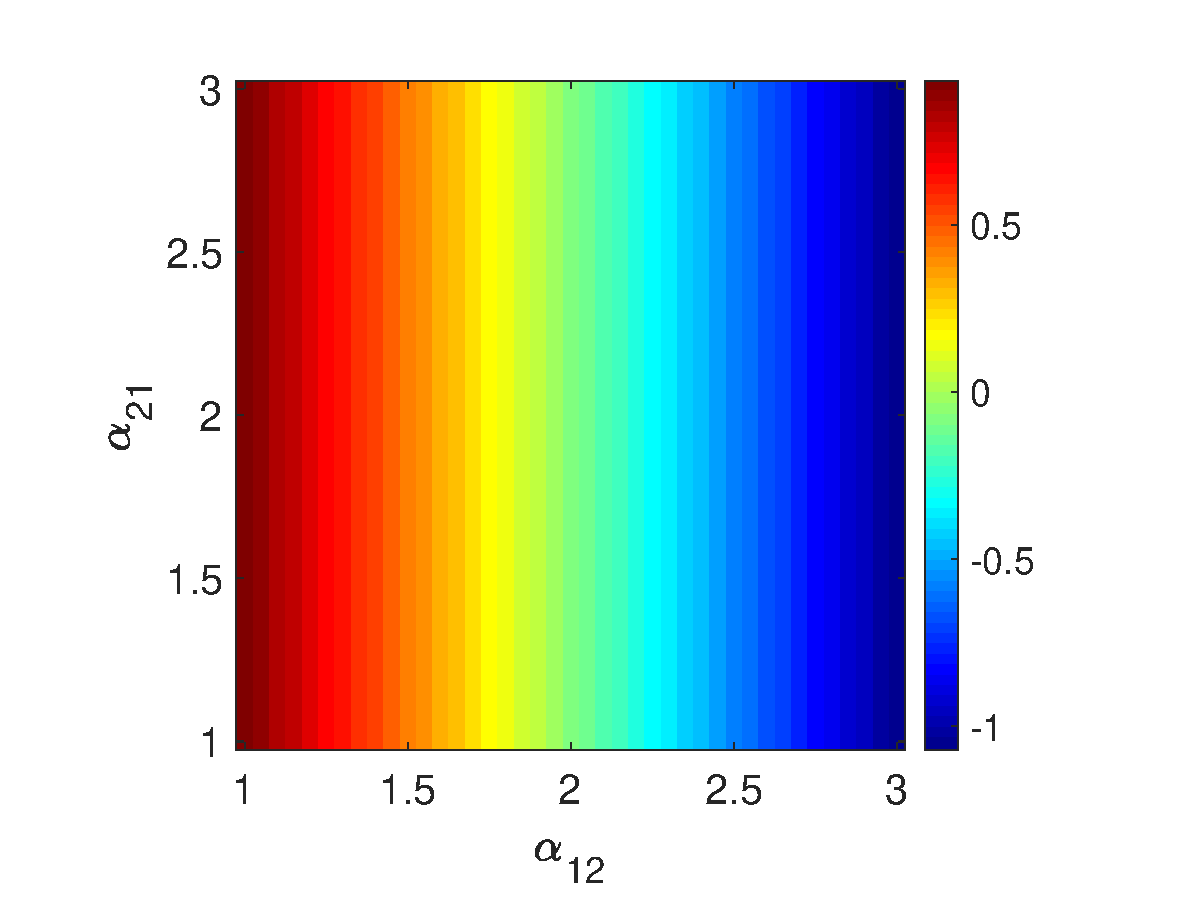
\includegraphics[width=1\linewidth]{Images/photo17_1.eps}
            \end{center}
        \end{minipage} 
        \begin{minipage}{0.32\linewidth}
            \begin{center}
                \includegraphics[width=1\linewidth]{Images/photo17_2.eps}
            \end{center}
        \end{minipage} 
    \begin{minipage}{0.32\linewidth}
        \begin{center}
            \includegraphics[width=1\linewidth]{Images/photo17_3.eps}
        \end{center}
    \end{minipage} 
  
  \caption{\textbf{Amplitude LS on the connectivity parameter space in symmetrical homogeneous two-cell networks.} Cell-1 and cell-2 oscillate with amplitude value 1.5. Left and middle: amplitude LS. For each pair of cross-connectivity parameters, there are the values of self-connectivity parameters, $\alpha_{11}$ (Left) and $\alpha_{22}$ (Middle), such as the network amplitude is preserved. Right: frequency for each point of the amplitude LS. Parameter values: $\lambda = 1$, $b=1$, $a = 1$, $\omega= 1$.}
  \label{photo17}
\end{figure}

The next statement summarizes the main features of amplitude and frequency LSs on the connectivity parameter space in symmetrical homogeneous two-cell networks.

\begin{Statement}
Symmetrical homogeneous networks show 2-dimensional amplitude level sets on the connectivity parameter space. Furthermore, the network frequency is constant throughout amplitude level sets on the connectivity parameter space. Consequently, symmetrical homogeneous networks show 2-dimensional total-degenerated level sets on the connectivity parameter space.
\end{Statement}

Symmetrical homogeneous networks are of interest because total-degenerated  LSs on the connectivity parameter space can be easily characterized. For a given pair of cross-connectivity parameter $\alpha_{12}$ and $\alpha_{21}$, compensated self-connectivity parameters $\alpha_{11}$ and $\alpha_{22}$ can be found in order to preserve a given network amplitude.

Fig (\ref{photo18}) shows how breaking the condition for LSs preservation in synchronized homogeneous networks, Eq. (\ref{e29}), affects individual amplitude and frequency LSs. Here, cross-connectivity parameter are fixed and self-connectivity parameters are perturbed from it LSs preserving value. Both self-connectivity parameters are perturbed the same amount so as to guarantee a symmetrical network. Top plots show the effect of mutually higher self-connectivity, whereas bottom plots shows the effect of mutually lower self-connectivity. 

\begin{figure}[h]
\centering
  \begin{minipage}{0.45\linewidth}
  \centering
    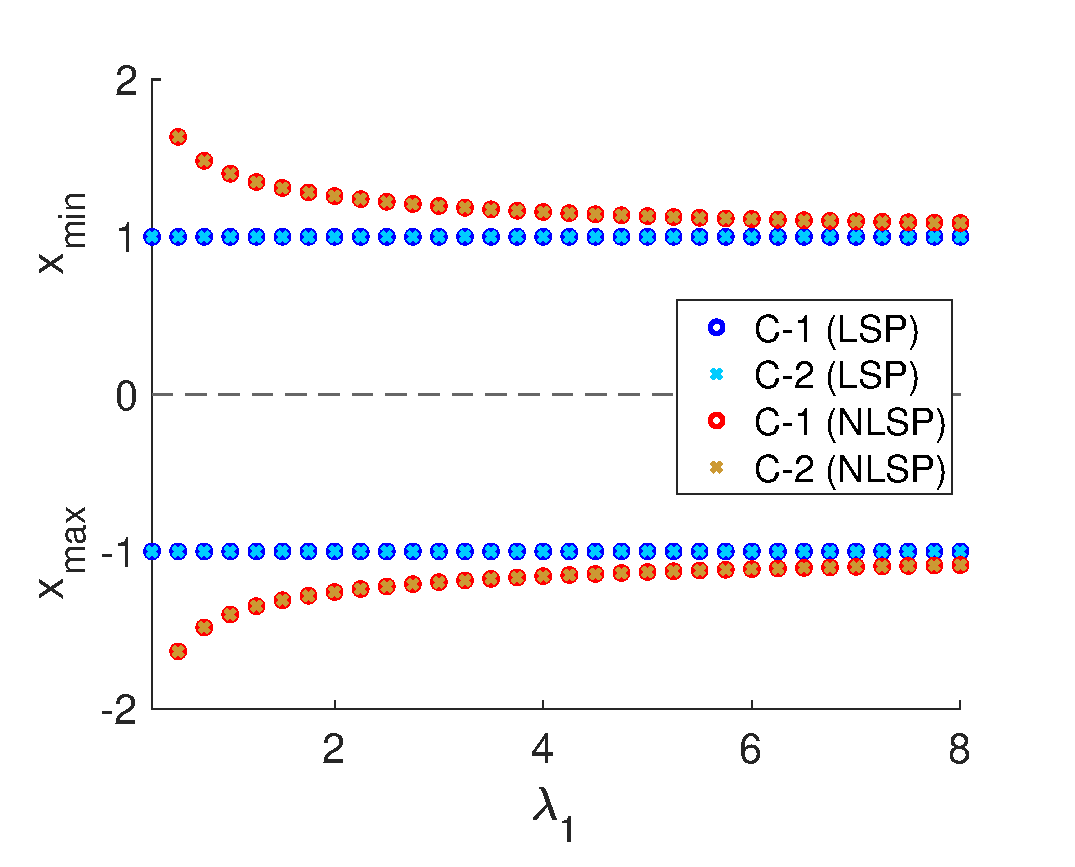
\includegraphics[width=1\linewidth]{Images/photo18_1.eps} 
  \end{minipage} 
  \begin{minipage}{0.45\linewidth}
  \centering
    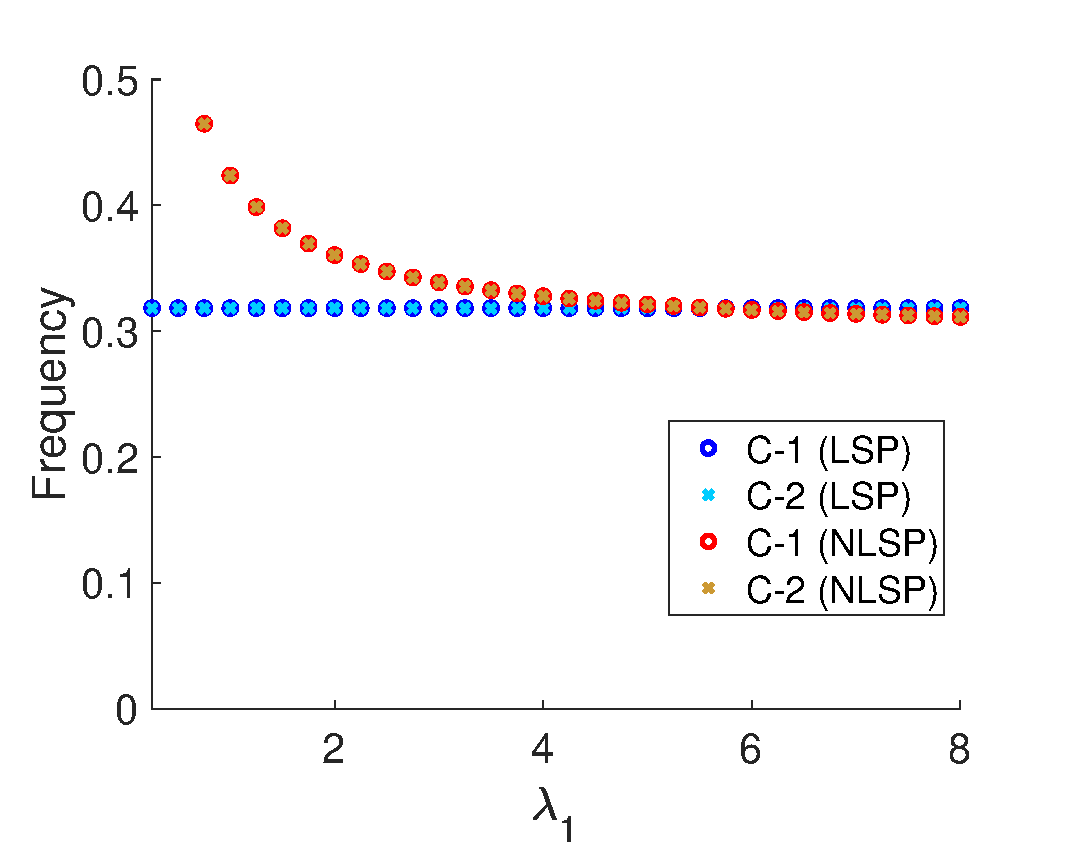
\includegraphics[width=1\linewidth]{Images/photo18_2.eps} 
  \end{minipage} 
  
  \begin{minipage}{0.45\linewidth}
  \centering
    \includegraphics[width=1\linewidth]{Images/photo18_3.eps} 
  \end{minipage} 
  \begin{minipage}{0.45\linewidth}
  \centering
    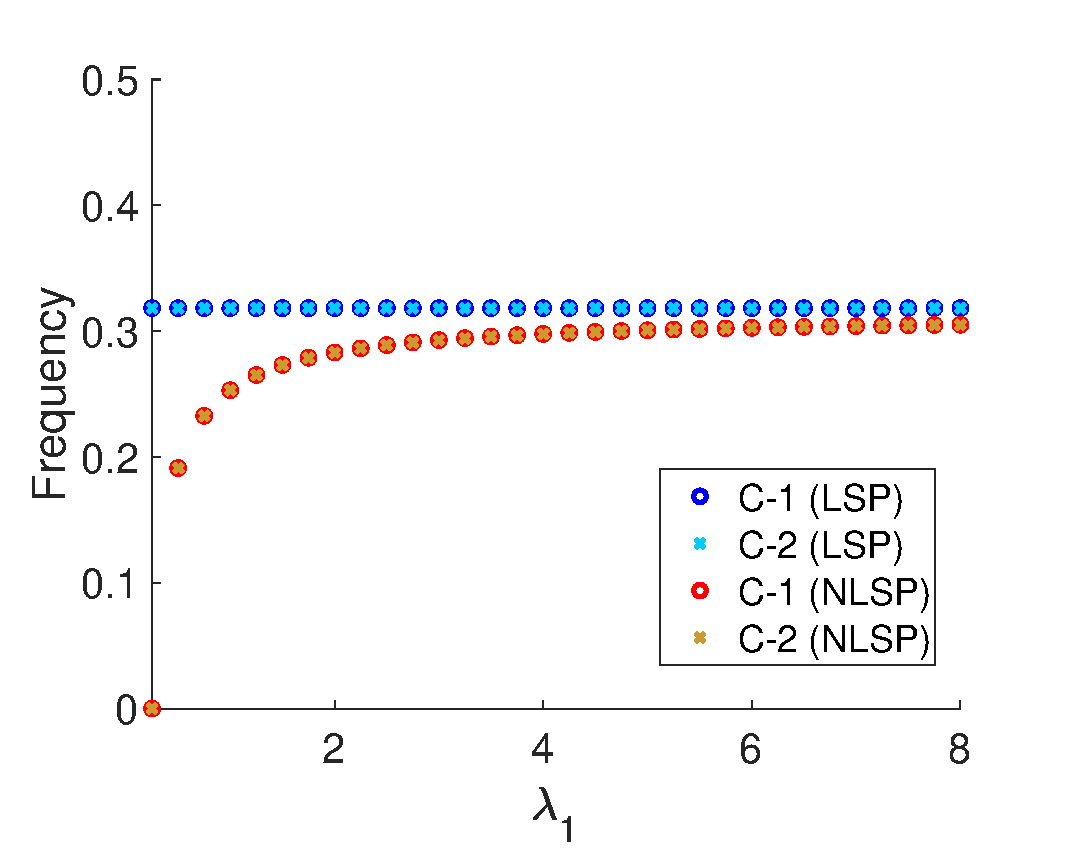
\includegraphics[width=1\linewidth]{Images/photo18_4.eps} 
  \end{minipage} 
  
    \caption{\textbf{Effect of mutually higher and lower self-connectivity (compared to the self-connectivity preserving individual LSs) on individual amplitude LSs in synchronized homogeneous networks.} Top: mutually higher self-connectivity. Parameter values: $a = 1$, $\omega = 1$, $\alpha_{12}=1$, $\alpha_{21}=1$, $\alpha_{11}=0.5$ and $\alpha_{22}=0.5$ (Perturbation: $+1.5$). Bottom: mutually lower self-connectivity. Parameter values: $a = 1$, $\omega = 1$, $\alpha_{12}=1$, $\alpha_{21}=1$, $\alpha_{11}=-1.75$ and $\alpha_{22}=-1.75$ (Perturbation $-0.75$). Left: amplitude  envelope  diagram  for values  $(\lambda,b)$  belonging  to the  same individual  amplitude  LS. Right: frequency  diagram  for  values  $(\lambda,b)$ belonging  to  the  same  individual  amplitude LS. LSP refers to the LS preserving network in which connectivity parameters preserve individual LSs. NLSP refers to perturbed networks in which self-connectivity parameters have been modified.}
  \label{photo18}
\end{figure}

In particular, we see that a mutual increase in self-connectivity leads to higher amplitude symmetrical networks, while a mutual decrease in self-connectivity produces symmetrical networks with lower amplitude values.

More specifically, for a given network amplitude value ($A_{\text{Net}}$), the network amplitude LS on connectivity parameter space is given by

\begin{equation}
    C_{A_{\text{Net}}} = 
    \begin{pmatrix}
        -\alpha_{12} + \varepsilon(A_{\text{Net}}) & \alpha_{12}\\
        \alpha_{21} & -\alpha_{21} + \varepsilon(A_{\text{Net}})
    \end{pmatrix}
    \text{ , } \hspace{0.5cm} \alpha_{12},\alpha_{21} \geq 0 \hspace{0.5cm} \text{or} \hspace{0.5cm}  \alpha_{12},\alpha_{21} \leq 0 
    \label{e37}
\end{equation}

where $\varepsilon(A_{\text{Net}})$ is a constant dependent on the network amplitude $A_{\text{Net}}$. Interestingly, the compensatory function associated with each self-connectivity parameter only depends on its corresponding cross-connectivity parameter. In other words, cross-connectivity parameter $\alpha_{12}$ only compensates self-connectivity parameter $\alpha_{11}$, while cross-connectivity parameter $\alpha_{21}$ only compensates self-connectivity parameter $\alpha_{22}$.

As it is expected, when the network amplitude equals the individual cell amplitude ($A_{Net} = A_{Ind}$), the network amplitude LS corresponds to the LS on the connectivity parameter space which preserve individual LSs, Eq. (\ref{e29}).

\subsubsection{Changing intrinsic parameters}
Since the network frequency ($f_{\text{Net}}$) is constant throughout amplitude LSs on the connectivity parameter space, there is a correspondence between a given network amplitude LS on connectivity parameter space and its frequency. If for a given network amplitude LS on connectivity parameter space, a different network frequency is required, intrinsic parameters must be changed. However, the network amplitude LS on connectivity parameter space might change. In other words, self-connectivity parameters might be differently compensated for a given pair of cross-connectivity parameters.

In Fig. (\ref{photo19}), we show the network frequency on the amplitude LS ($A_{\text{Net}} = 1.5$) on connectivity parameter space as a function of parameters $\lambda$ and $b$. We also compare the network frequency ($f_{\text{Net}}$) with the individual cell frequency ($f_{\text{Ind}}$).

\begin{figure}[h]
  \begin{minipage}{0.32\linewidth}
            \begin{center}
             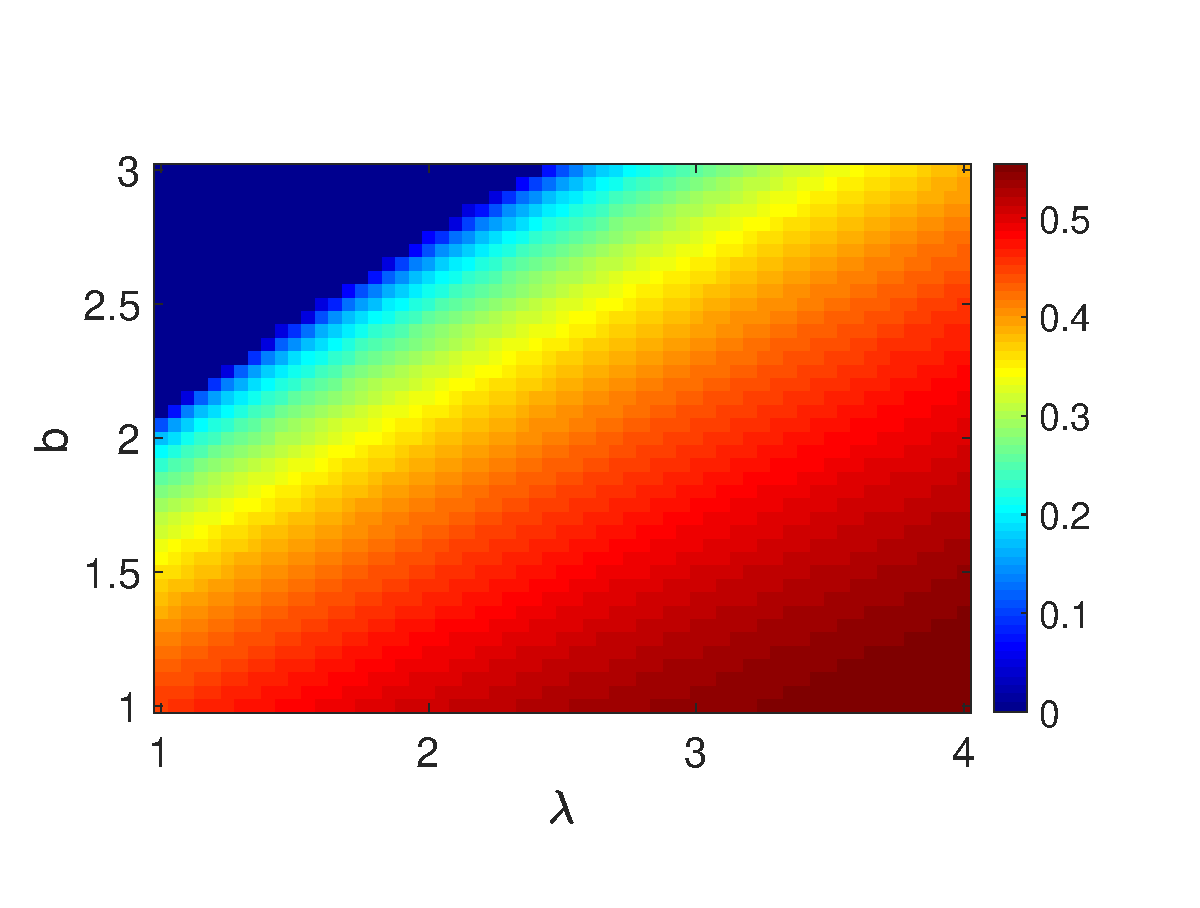
\includegraphics[width=1\linewidth]{Images/photo19_1.eps}
            \end{center}
        \end{minipage} 
        \begin{minipage}{0.32\linewidth}
            \begin{center}
                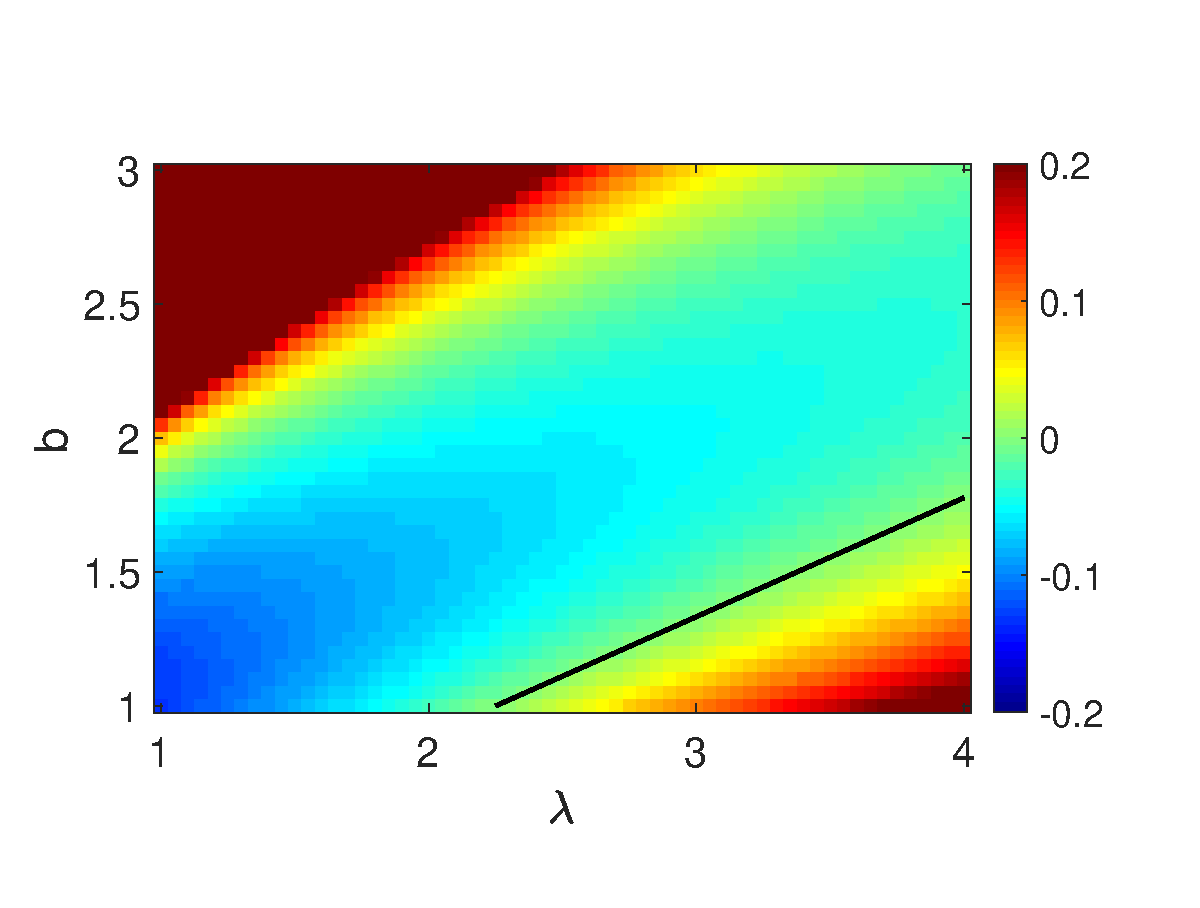
\includegraphics[width=1\linewidth]{Images/photo19_2.eps}
            \end{center}
        \end{minipage} 
        \begin{minipage}{0.32\linewidth}
            \begin{center}
                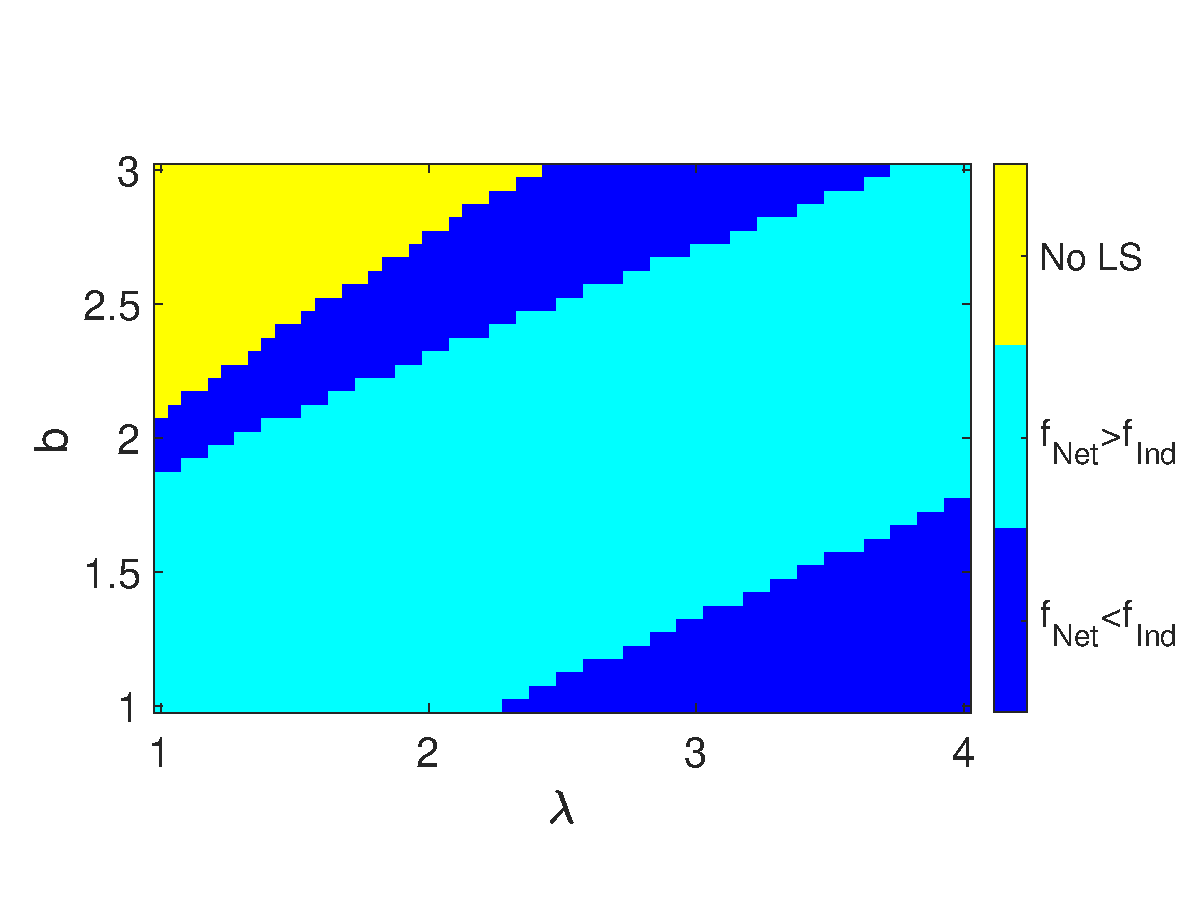
\includegraphics[width=1\linewidth]{Images/photo19_3.eps}
            \end{center}
        \end{minipage} 
  \caption{\textbf{Intrinsic parameters change the value of the network frequency preserved on a given amplitude LS on connectivity parameter space.} Both cells oscillate with amplitude value 1.5 ($A_{\text{Net}} = 1.5$). Left: network frequency on the amplitude LS ($A_{\text{Net}} = 1.5$) on connectivity parameter space as a function of parameters $\lambda$ and $b$. Middle: the difference between the individual cell frequency and the network frequency (from left). The blank line represents the case in which the individual LS ($K_{a}=2.25$ and $K_{f} = 3.25$) is preserved. Right: regions where the network frequency is higher or lower than the individual cell frequency (from Middle). Parameter values: $a = 1$, $\omega = 1$, $\alpha_{12} = 1$ and $\alpha_{21}=1$.}
  \label{photo19}
\end{figure}

Curves preserving the frequency in Fig. (\ref{photo19})-Left represent 1-dimensional total-degenerated LSs on the $\lambda-b-\alpha_{11}-\alpha_{22}$ parameter space. As an exception, black line in (\ref{photo19})-Middle is the only curve in which the value of self-connectivity parameters $\alpha_{11}$ and $\alpha_{22}$ does not change (same amplitude LS on connectivity parameter space). It corresponds to the case where individual LS are preserved in the two-cell network. 

\subsection{Non-symmetrical Networks}
In non-symmetrical homogeneous networks, the amplitude value of each cell on a given amplitude LS is different. Fig. (\ref{photo20}) shows an example of an amplitude LS ($A_{1} = 1.5$ and $A_{2}=1.25$) in a non-symmetrical homogeneous networks for representative parameter values. It is also shown the network frequency for each point in the amplitude LS.

\begin{figure}[h]
  \begin{minipage}{0.32\linewidth}
  \begin{center}
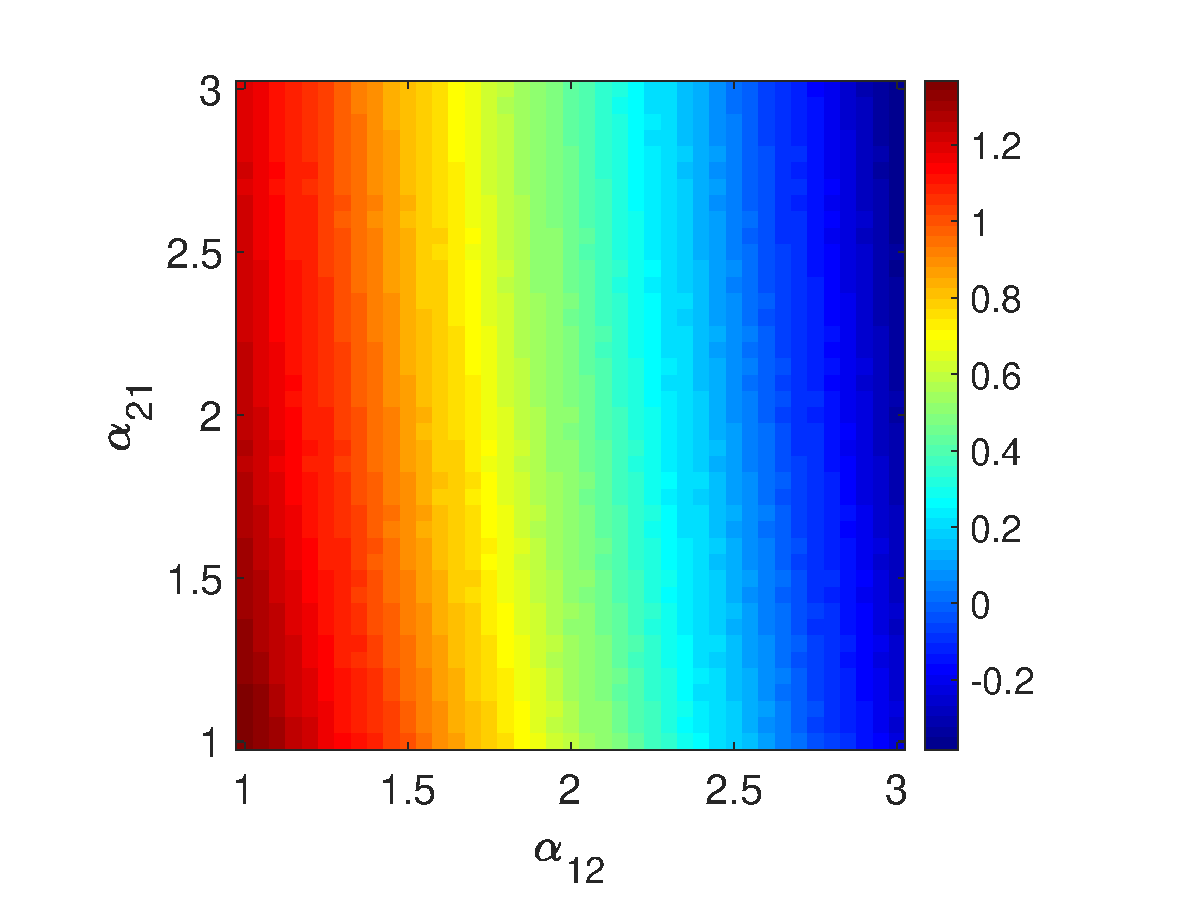
\includegraphics[width=1\linewidth]{Images/photo20_1.eps}
\end{center}
  \end{minipage} 
  \begin{minipage}{0.32\linewidth}
  \begin{center}
\includegraphics[width=1\linewidth]{Images/photo20_2.eps}
\end{center}

  \end{minipage} 
   \begin{minipage}{0.32\linewidth}
  \begin{center}
\includegraphics[width=1\linewidth]{Images/photo20_3.eps}
\end{center}

  \end{minipage} 
  
   \caption{\textbf{Amplitude LS on the connectivity parameter space in non-symmetrical homogeneous two-cell networks.} Cell-1 oscillates with amplitude value 1.5, while cell-2 oscillates with amplitude value 1.25. Left and middle: Amplitude LS. For each pair of cross-connectivity parameters, there are the values of self-connectivity parameters, $\alpha_{11}$ (Left) and $\alpha_{22}$ (Middle), such as both the amplitude value of each cell in the network is preserved. Right: Frequency for each point of the amplitude LS. Parameter values: $\lambda = 1$, $b=1$, $a = 1$, $\omega= 1$.}
  \label{photo20}
\end{figure}

The next statement summarizes the main properties of amplitude LSs on the connectivity parameter space in non-symmetrical homogeneous networks.

\begin{Statement}
Non-symmetrical homogeneous networks show 2-dimensional amplitude level sets on the connectivity parameter space. However, the network frequency is not constant throughout amplitude level sets on the connectivity parameter space. Consequently, non-symmetrical homogeneous networks show 1-dimensional total-degenerated level sets on the connectivity parameter space.
\end{Statement}

The fact that the network frequency is not preserve throughout amplitude LSs on the connectivity parameter in non-symmetrical homogeneous networks is the main difference between non-symmetrical and symmetrical homogeneous networks.

\section{Type-\textrm{I} Heterogeneous Two-cell Networks}
We consider type-\textrm{I} heterogeneous networks in which cells belong to the same individual amplitude and frequency LS. Contrary to homogeneous networks, we found that symmetrical and non-symmetrical type-\textrm{I} heterogeneous networks show similar properties. For the sake of simplicity, we illustrate them in a symmetrical type-\textrm{I} heterogeneous network.

\subsection{Connectivity parameter space}

Fig. (\ref{photo21}) shows how breaking the condition for LSs preservation in type-\textrm{I} heterogeneous networks, Eq. (\ref{e29}), affects individual amplitude and frequency LSs. Here, cross-connectivity parameter are fixed and self-connectivity parameters are perturbed from it LSs preserving value. Both self-connectivity parameters are perturbed the same amount so as to see the differences between symmetrical homogeneous and symmetrical type-\textrm{I} heterogeneous networks. Top plots show the effect of mutually higher self-connectivity, whereas bottom plots shows the effect of mutually lower self-connectivity. 

\begin{figure}[h]
\centering
  \begin{minipage}{0.45\linewidth}
  \begin{center}
\includegraphics[width=1\linewidth]{Images/photo21_1.eps}
\end{center}
  \end{minipage} 
  \begin{minipage}{0.45\linewidth}
  \begin{center}
\includegraphics[width=1\linewidth]{Images/photo21_2.eps}
\end{center}
\end{minipage} 
 \begin{minipage}{0.45\linewidth}
  \begin{center}
\includegraphics[width=1\linewidth]{Images/photo21_3.eps}
\end{center}
  \end{minipage} 
  \begin{minipage}{0.45\linewidth}
  \begin{center}
\includegraphics[width=1\linewidth]{Images/photo21_4.eps}
\end{center}
\end{minipage} 
   \caption{\textbf{Effect of mutually higher and lower self-connectivity (compared to the self-connectivity preserving individual LSs) on individual amplitude LSs in synchronized type-\textrm{I} heterogeneous networks.} Top: mutually higher self-connectivity. Parameter values:$\lambda_{2}=1$, $b_{2}=1$, $a = 1$, $\omega = 1$, $\alpha_{12}=1$, $\alpha_{21}=1$, $\alpha_{11}=0.5$ and $\alpha_{22}=0.5$ (Perturbation: $+1.5$). Bottom: mutually lower self-connectivity. Parameter values: $\lambda_{2}=1$, $b_{2}=1$, $a = 1$, $\omega = 1$, $\alpha_{12}=1$, $\alpha_{21}=1$, $\alpha_{11}=-1.75$ and $\alpha_{22}=-1.75$ (Perturbation $-0.75$). Left: amplitude  envelope  diagram  for values  $(\lambda_{1},b_{1})$  belonging  to the  same individual  amplitude LS. Right: frequency  diagram  for  values  $(\lambda_{1},b_{1})$ belonging  to  the  same  individual  amplitude LS. LSP refers to the LS preserving network in which connectivity parameters preserve individual LSs. NLSP refers to perturbed networks in which self-connectivity parameters have been modified.}
  \label{photo21}
\end{figure}

Contrary to homogeneous networks, the amplitude value of each cell in the network is different. In Fig. (\ref{photo21}), the only case in which amplitude values coincide is when cells are identical, which corresponds to the homogeneous network case.

Fig. (\ref{photo22}) shows an example of an amplitude LS ($A_{Net} = 1.5$) on the connectivity parameter space in a type-\textrm{I} heterogeneous network ($K_{a}=1$).

\begin{figure}[h]
  \begin{minipage}{0.32\linewidth}
  \begin{center}
\includegraphics[width=1\linewidth]{Images/photo22_1.eps}
\end{center}
  \end{minipage} 
  \begin{minipage}{0.32\linewidth}
  \begin{center}
\includegraphics[width=1\linewidth]{Images/photo22_2.eps}
\end{center}

  \end{minipage} 
   \begin{minipage}{0.32\linewidth}
  \begin{center}
\includegraphics[width=1\linewidth]{Images/photo22_3.eps}
\end{center}

  \end{minipage} 
  
   \caption{\textbf{Amplitude LS on the connectivity parameter space in symmetrical type-\textrm{I} heterogeneous two-cell network.} Both cells oscillate with amplitude value 1.5. Left and middle: amplitude LS. For each pair of cross-connectivity parameters, there are the values of self-connectivity parameters, $\alpha_{11}$ (Left) and $\alpha_{22}$ (Middle), such as the amplitude value of each cell in the network is preserved. Right: frequency for each point on the amplitude LS. Parameter values: $\lambda_{1} = 1$, $b_{1}=1$, $\lambda_{2}=3$, $b_{2}=3$, $a_{1} = 1$, $\omega_{1} = 1$, $a_{2}=1$ and $\omega_{2}=1$.}
  \label{photo22}
\end{figure}

The next statement summarizes the main properties of network LSs on the connectivity parameter space in type-\textrm{I} heterogeneous network. We note that LSs properties in type-\textrm{I} heterogeneous network are the same as LSs properties in non-symmetrical homogeneous networks.

\begin{Statement}
Type-\textrm{I} heterogeneous networks show 2-dimensional amplitude level sets on the connectivity parameter space. However, the network frequency is not constant throughout amplitude level sets on the connectivity parameter space. Consequently, type-\textrm{I} heterogeneous networks show 1-dimensional total-degenerated level sets on the connectivity parameter space.
\end{Statement}

The representative amplitude LS on the connectivity parameter space shown in Fig. (\ref{photo22}) is parametrized by cross-connectivity parameters. We focus on the compensatory relations between compensating parameters $\alpha_{12}$ and $\alpha_{21}$ and compensated parameters $\alpha_{11}$ and $\alpha_{22}$.

Fig. (\ref{photo23}) shows how connectivity parameter are compensated when cross-connectivity parameters are changed in order to preserve the network attributes. Furthermore, voltage traces are shown for two different point on the 1-dimensional total-degenerated LS.

\begin{figure}[h]
  \begin{minipage}{0.32\linewidth}
  \begin{center}
\includegraphics[width=1\linewidth]{Images/photo23_1.eps}
\end{center}
  \end{minipage} 
  \begin{minipage}{0.32\linewidth}
  \begin{center}
\includegraphics[width=1\linewidth]{Images/photo23_2.eps}
\end{center}

  \end{minipage} 
   \begin{minipage}{0.32\linewidth}
  \begin{center}
\includegraphics[width=1\linewidth]{Images/photo23_3.eps}
\end{center}

  \end{minipage} 
  
   \caption{\textbf{Total-degenerated LS on the connectivity parameter space.} Network amplitude, $A_{\text{Net}} = 1.5$ and network frequency, $f_{\text{Net}} = 0.37$. Left: total-degenerated LS parametrized by either cross-connectivity parameter. Black line represents the projection of compensated self-connectivity parameters onto the cross-connectivity parameter space. Middle: voltage traces at the point of the LS with $\alpha_{12}=0.7$. Left: voltage traces at the point of the LS with $\alpha_{12}=2.2$. Parameter values: $\lambda_{1} = 1$, $b_{1}=1$, $\lambda_{2}=3$, $b_{2}=3$, $a_{1} = 1$, $\omega_{1} = 1$, $a_{2}=1$ and $\omega_{2}=1$.}
  \label{photo23}
\end{figure}

As it is shown, the increase of any self-connectivity parameter leads to a decrease in its corresponding self-connectivity parameter. For instance, if parameter $\alpha_{12}$ increases, the self-connectivity parameter $\alpha_{11}$ decreases. In addition, the increase of any cross-connectivity parameter leads to an increase in the other cross-connectivity parameter. These compensations are shown in Figure (\ref{photo23})-Left.

Voltage traces seems to preserve their pattern along the total-degenerated LS on the connectivity parameter space shown in Figure (\ref{photo23})-Left, but a significant change in the phase difference is observed.


\subsection{Changing intrinsic parameters}
Finally, we study the dependence between the network frequency on amplitude LSs on connectivity parameter space and intrinsic parameters. Regions on each amplitude LS in which the network frequency is higher and lower than the individual cell frequency are compared. Since the network is type-\textrm{I} heterogeneous, cells do have the same amplitude and frequency value.

Cross-connectivity parameters $\alpha_{12}$ and $\alpha_{21}$ will be the compensating parameters and amplitude LSs on the connectivity parameters space for the same values on the cross-connectivity parameter space (same subspace) are compared.

Fig. (\ref{photo24}) shows the network frequency on several amplitude LSs ($A_{\text{Net}} = 1.5$) for different type-\textrm{I} heterogeneous networks in which cells belong to different points on the individual amplitude LS with $K_{a}=1$. For each amplitude LS, the dark blue region represents point of the amplitude LS in which the network frequency is higher than the individual cell frequency while the light blue region represents point of the amplitude LS in which the network frequency is lower.

\begin{figure}[h]
\centering
  \begin{minipage}{0.32\linewidth}
  \begin{center}
\includegraphics[width=1\linewidth]{Images/photo24_1.eps}
\end{center}
  \end{minipage} 
  \begin{minipage}{0.32\linewidth}
  \begin{center}
\includegraphics[width=1\linewidth]{Images/photo24_2.eps}
\end{center}

  \end{minipage} 
   \begin{minipage}{0.32\linewidth}
  \begin{center}
\includegraphics[width=1\linewidth]{Images/photo24_3.eps}
\end{center}
  \end{minipage} 
  
   \begin{minipage}{0.32\linewidth}
  \begin{center}
\includegraphics[width=1\linewidth]{Images/photo24_4.eps}
\end{center}
  \end{minipage} 
  \begin{minipage}{0.32\linewidth}
  \begin{center}
\includegraphics[width=1\linewidth]{Images/photo24_5.eps}
\end{center}

  \end{minipage} 
   \begin{minipage}{0.32\linewidth}
  \begin{center}
\includegraphics[width=1\linewidth]{Images/photo24_6.eps}
\end{center}
  \end{minipage} 
  
   \begin{minipage}{0.32\linewidth}
  \begin{center}
\includegraphics[width=1\linewidth]{Images/photo24_7.eps}
\end{center}
  \end{minipage} 
  \begin{minipage}{0.32\linewidth}
  \begin{center}
\includegraphics[width=1\linewidth]{Images/photo24_8.eps}
\end{center}

  \end{minipage} 
   \begin{minipage}{0.32\linewidth}
  \begin{center}
\includegraphics[width=1\linewidth]{Images/photo24_9.eps}
\end{center}
  \end{minipage} 
  
   \caption{\textbf{Intrinsic parameter in type-\textrm{I} heterogeneous two-cell network have an overall effect on the network frequency on amplitude LSs on the connectivity parameter space.} Both cells oscillate with amplitude value 1.5. Both cells belong to different points of the individual amplitude LS with $K_{a}=1$. Rows: cell-2 moves along its individual amplitude LS. Columns: cell-1 moves along its individual amplitude LS. Dark blue represent points in the amplitude LS for which the network amplitude is higher than the individual cell frequency while light blue represents points in the amplitude LS for which the network amplitude is lower than the individual cell frequency. Parameter values: $a_{1} = 1$, $\omega= 1$, $a_{2}=1$ and $\omega_{2}=1$.}
  \label{photo24}
\end{figure}

As a result, as intrinsic parameters $\lambda_{1}$ or $\lambda_{2}$ are higher (cell-1 or cell-2 moves along its individual amplitude LS towards higher values of $\lambda_{1}$ or $\lambda_{2}$), the network frequency on amplitude LSs on the connectivity parameter space decreases and take lower values.

We note that although connectivity parameter are able to change the network frequency on a given amplitude LS, a greater effect on the network frequency is observed when intrinsic parameters $\lambda_{1}$ or $\lambda_{2}$ are changed. Moreover, total degenerated LSs could be found on the $\lambda_{1}-\lambda_{2}-\alpha_{11}-\alpha_{22}$ parameter space as well.


\section{Type-\textrm{II} Heterogeneous Two-cell Networks}
Type-\textrm{II} heterogeneous networks represent the most general network, in which cells belong to different individual amplitude and frequency LSs. Therefore, cells do have different individual amplitude and frequencies values. We will not distinguish between symmetrical and non-symmetrical type-\textrm{II} heterogeneous networks since they show the same network attribute LSs properties.

Firstly, we start characterizing LSs on the connectivity parameter space. Afterwards, we study LSs on the intrinsic parameter space of a single cell. We will study whether or not network attributes can be maintained if only intrinsic parameters of a cell in the network are changed. Finally we show total-degenerated network LSs on a mixed parameter space involving intrinsic parameters from both cells.

\subsection{Connectivity parameter space}
Fig. (\ref{photo25}) shows an example of an amplitude LS ($A_{\text{Net}}$ = 1.5) in an type-\textrm{II} heterogeneous network for representative parameter values. It is also shown the network frequency for each point on the amplitude LS.

\begin{figure}[h]
  \begin{minipage}{0.32\linewidth}
  \begin{center}
\includegraphics[width=1\linewidth]{Images/photo25_2.eps}
\end{center}
  \end{minipage} 
  \begin{minipage}{0.32\linewidth}
  \begin{center}
\includegraphics[width=1\linewidth]{Images/photo25_1.eps}
\end{center}

  \end{minipage} 
   \begin{minipage}{0.32\linewidth}
  \begin{center}
\includegraphics[width=1\linewidth]{Images/photo25_3.eps}
\end{center}

  \end{minipage} 
  
  \caption{\textbf{Amplitude LS on the connectivity parameter space in type-\textrm{II} heterogeneous two-cell network.} Both cells oscillate with amplitude value 1.5. Left and Middle: amplitude LS. For each pair of cross-connectivity parameters, there are the values of self-connectivity parameters, $\alpha_{11}$ (Left) and $\alpha_{22}$ (Middle), such as both the amplitude value of each cell in the network is preserved. Right: frequency for each point of the amplitude LS. Parameter values: $\lambda_{1} = 1$, $b_{1}=1$, $a_{1} = 1$, $\omega_{1} = 1$, $\lambda_{2} = 3$, $b_{2}=1$, $a_{2} = 1$, $\omega_{2} = 1$.}
  \label{photo25}
\end{figure}

The next Statement summarizes the main LSs properties on the connectivity parameter space in type-\textrm{II} heterogeneous networks.

\begin{Statement}
Type-\textrm{II} heterogeneous networks show 2-dimensional amplitude level sets on the connectivity parameter space. However, the network frequency is not constant throughout amplitude level sets on the connectivity parameter space. Consequently, type-\textrm{II} heterogeneous networks show 1-dimensional total-degenerated level sets on the connectivity parameter space.
\end{Statement}

We note type-\textrm{I} and type-\textrm{II} heterogeneous networks show similar network LSs properties on the connectivity parameter space. Both show 1-dimensional total-generated LSs on the connectivity parameter space.

\subsection{The intrinsic parameter space of a single cell}
An interesting question in type-\textrm{II} heterogeneous networks is whether intrinsic parameters of a cell can be changed preserving network attributes. In other words, is it possible to find total-degenerated LSs on the intrinsic parameter space of a single cell?. Without loss of generality we consider the $\lambda_{1}-b_{1}-\omega_{1}-a_{1}$ parameter space, which corresponds to the intrinsic parameter space of cell-1.

Fig. (\ref{photo26}) shows an example of a LS on the  $\lambda_{1}-b_{1}-\omega_{1}-a_{1}$ parameter space preserving the network frequency ($f_{\text{Net}}$) and amplitude of cell-1 ($A_{1}$). It is also shown the amplitude value of cell-2 ($A_{2}$) for each point on the LS. In particular, curves on the LS preserving the amplitude value of cell-2 represent total-degenerated LSs on the intrinsic parameter space of cell-1.

\begin{figure}[h]
  \begin{minipage}{0.32\linewidth}
  \begin{center}
\includegraphics[width=1\linewidth]{Images/photo26_1.eps}
\end{center}
  \end{minipage} 
  \begin{minipage}{0.32\linewidth}
  \begin{center}
\includegraphics[width=1\linewidth]{Images/photo26_2.eps}
\end{center}
  \end{minipage} 
   \begin{minipage}{0.32\linewidth}
  \begin{center}
\includegraphics[width=1\linewidth]{Images/photo26_3.eps}
\end{center}

  \end{minipage} 
  
  \caption{\textbf{Total-degenerated LS on the $\lambda_{1}-b_{1}-\omega_{1}-a_{1}$ parameter space.} Both cells oscillate with amplitude value 1.5. Left and middle: LS preserving the network frequency and the amplitude of cell-1. For each pair parameters $a_{1}$ and $b_{1}$, there are the values of parameters $\lambda_{1}$ (Left) and $\omega_{1}$ (Middle), such as the amplitude value of cell-1 and the frequency network is preserved. Right: amplitude value of cell-2 for each point of the LS. Parameter values: $\lambda_{2} = 1$, $b_{2}=1$, $a_{2} = 1$, $\omega_{2} = 1$, $\alpha_{12}=2$, $\alpha_{21}=2$, $\alpha_{11}=0$ and $\alpha_{22}=0$.}
  \label{photo26}
\end{figure}

The next statement summarizes the main properties of attribute LSs on the intrinsic parameter space of a single cell.

\begin{Statement}
The two-cell network shows 2-dimensional level sets on the intrinsic parameter space of a single cell preserving the attributes (frequency and amplitude) of that cell in the network. However, the amplitude value of the other cell is not constant on each level set. Consequently, the two-cell network shows 1-dimensional total-degenerated level sets on the intrinsic parameter space of a single cell ($\lambda_{1}-b_{1}-\omega_{1}-a_{1}$ or $\lambda_{2}-b_{2}-\omega_{2}-a_{2}$ parameter spaces).
\end{Statement}

In order to gain insight on the different parameter compensations, Fig. (\ref{photo27}) shows in more detail the corresponding compensatory relations leading to total-degenerated LS on the intrinsic parameter space of a single cell.

\begin{figure}[h]
  \begin{minipage}{0.32\linewidth}
  \begin{center}
\includegraphics[width=1\linewidth]{Images/photo27_1.eps}
\end{center}
  \end{minipage} 
  \begin{minipage}{0.32\linewidth}
  \begin{center}
\includegraphics[width=1\linewidth]{Images/photo27_2.eps}
\end{center}

  \end{minipage} 
   \begin{minipage}{0.32\linewidth}
  \begin{center}
\includegraphics[width=1\linewidth]{Images/photo27_3.eps}
\end{center}

  \end{minipage} 
  
     \caption{\textbf{Total-degenerated LS on the connectivity parameter space of a single cell.} Network amplitude, $A_{\text{Net}} = 1.5$ and network frequency, $f_{\text{Net}} = 0.45$. Left: total-degenerated LS parametrized by either parameter $b_{1}$ or $a_{1}$. Black line represents the projection of compensated parameters $\lambda_{1}$ and $\omega_{1}$ onto the $a_{1}-b_{1}$ parameter space. Middle: voltage traces at the point of the LS with $\alpha_{12}=0.7$. Left: voltage traces at the point of the LS with $\alpha_{12}=2.2$. Parameter values: $\lambda_{2}=1$, $b_{2}=1$, $a_{2} = 1$, $\omega_{2} = 1$, $\alpha_{11}=0$, $\alpha_{22}=0$, $\alpha_{12}=1$ and $\alpha_{21}=1$.}
  \label{photo27}
\end{figure}

It is shown the differences on the compensatory relations between parameters. While parameters $\lambda_{1}$ and $b_{1}$ have a positive compensation (if one increases the other increases or vice versa), parameters $\omega_{1}$ and $a_{1}$ have a negative compensation (if one increases the other decreases or vice versa). This type of compensation relations was also seen at the individual neuron level, Eqs. (\ref{e16}) and (\ref{e18}). However, new dependencies are observed between parameters. More specifically, parameters $a_{1}$ and $b_{1}$ compensate each other. An increase in parameter $a_{1}$ induces an increase in parameter $b_{1}$, or vice versa. This compensatory relation is shown in Fig. (\ref{photo27})-Left (Black curve).

Moreover, Fig. (\ref{photo27}) also shows voltage traces for two different points in the total-degenerated LS considered. Some slight differences are observed, but in contrast to total-degenerated LSs on the connectivity parameter space no significant change in phase difference is observed.

\subsection{Combined parameter space}
As a final result, we consider the combined $\lambda_{1}-b_{1}-\lambda_{2}-b_{2}$ parameter space. It involves intrinsic parameters from both cells in the network. We characterize total-degenerated LSs in this parameter space.

Fig. (\ref{photo28}) shows an example of a network amplitude LS ($A_{\text{Net}}=1$) on the $\lambda_{1}-b_{1}-\lambda_{2}-b_{2}$ parameter space. It is parametrized in terms of compensating parameters $\lambda_{1}$ and $\lambda_{2}$. It is also shown the network frequency for each point on the LS. In particular, curves on the amplitude LSs preserving the network frequency represent total-degenerated LSs on the $\lambda_{1}-b_{1}-\lambda_{2}-b_{2}$ parameter space.

\begin{figure}[h]
  \begin{minipage}{0.32\linewidth}
  \begin{center}
\includegraphics[width=1\linewidth]{Images/photo28_1.eps}
\end{center}
  \end{minipage} 
  \begin{minipage}{0.32\linewidth}
  \begin{center}
\includegraphics[width=1\linewidth]{Images/photo28_2.eps}
\end{center}

  \end{minipage} 
   \begin{minipage}{0.32\linewidth}
  \begin{center}
\includegraphics[width=1\linewidth]{Images/photo28_3.eps}
\end{center}

  \end{minipage} 
  
  \caption{\textbf{Total-degenerated LSs on the $\lambda_{1}-b_{1}-\lambda_{2}-b_{2}$ parameter space.} Both cells oscillate with amplitude value 1. Left/Middle: amplitude LS on the $\lambda_{1}-b_{1}-\lambda_{2}-b_{2}$ parameter space. For each pair of $\lambda_{1}$ and $\lambda_{2}$, there are the values of parameters, $b_{1}$ (Left) and $b_{2}$ (Middle), such as the amplitude of each cell is preserved. Right: frequency in each point in the amplitude LS. Parameter values: $a_{1} = 1$, $\omega_{1} = 1$, $a_{2} = 1$, $\omega_{2} = 1$, $\alpha_{12} = 1$, $\alpha_{21} = 1$, $\alpha_{11} = 0$ and $\alpha_{22} = 0$.}
  \label{photo28}
\end{figure}

The next statement summarizes the main properties of network total-degenerated LSs on the $\lambda_{1}-b_{1}-\lambda_{2}-b_{2}$ parameter space.

\begin{Statement}
Two-cell networks show 1-dimensional total-degenerated level sets on the $\lambda_{1}-b_{1}-\lambda_{2}-b_{2}$ parameter space. Furthermore, total-degenerated level sets are closed curves.
\end{Statement}

Interestingly, when considered a combined parameter space involving intrinsic parameter from both cells in the network, closed curves representing total-degenerated LSs are found.   % INCLUDE: introduction
\chapter{Conclusion}
\label{sec:con}
\section{Discussion}
In Chapter \ref{sec:results1}, we showed that attribute LSs are preserved in type-I and type-II heterogeneous networks only when individual cells belong to the same frequency LS. However, only when the network is type-I heterogeneous (cells belong to the same frequency and amplitude LSs) gap-junctions preserve individual attribute LSs. In other words, in networks in which cells belong to different amplitude LSs (type-II heterogeneous) gap-junctions do not preserve individual attribute LSs. In this case, the self-connectivity of each cell has to be readjusted in order to guarantee individual LSs preservation. More specifically, the cell with lower individual amplitude value needs higher self-inhibition, whereas the cell with higher individual amplitude value needs lower self-inhibition.

Moreover, we showed that as the network is more complex (it evolves from the type-I heterogeneous case to the most general type-II heterogeneous case), the symmetrical connectivity structure preserving LSs (gap-junctions) is broken until the point in which the network connectivity is unable to continue preserving individual attribute LSs (type-II with cells belonging to different frequency LSs). One question arises: taking into account that the single neuron model considered has a high degree of symmetries, which most probably lead to the fact that the symmetrical gap-junction connectivity preserve attribute LSs in the type-I heterogeneous networks, what would happen in neuronal models with lower degree of symmetries?. 

It might be reasonably that when symmetries are broken, the LS structure evolve from the “organized” structure shown in the $\Lambda \Omega_{2}$ model, to a “non-organized” structure in which each model parameter affects the value of any attribute. It would be something similar to what happens when the individual cell is self-connected (Chapter \ref{sec:results2}). In this scenario, it is likely that the whole individual LS structure will not be preserved, but some attribute LSs could be preserved, as it was shown in \cite{Iii2019}.

Results from \cite{Iii2019} shown that frequency LSs (on a two-dimensional parameter space) in two electrically (gap-junctions) coupled realistic biophysical networks (with cells belonging to the same frequency LS) are preserved. We note that the same feature is observed in the two-cell network, since attribute LSs are preserved in type-I heterogeneous networks.

In Chapter \ref{sec:results2}, we computed several network attribute LSs on different parameter spaces, involving the connectivity parameter space or the intrinsic parameter space of a single cell. Moreover, it was mentioned that more total-degenerated network LSs could be found in other parameter spaces, for example parameter spaces involving both connectivity parameters and intrinsic parameters. For the sake of simplicity, we reduced our analysis to study until 4-dimensional parameter spaces, although higher dimensional parameter spaces could be considered. 

Nevertheless, we have verified one of the main prediction done in  \cite{Oly}. They predict that if a particular homeostatic mechanism maintain m independent characteristics (or attributes) of neural activity, then at least m parameters must be changed as a response to a perturbation in one parameter of the system. For instance, 2-dimensional total-degenerated LSs on the intrinsic parameter space in the self-connected cell verify that statement. 

However, two-cell networks seems not to verify predictions in  \cite{Oly}. Several total-degenerated LSs have been computed preserving the amplitude value of each cell and the frequency value of each cell in the network (an overall of 4 attributes or characteristics). We must mention that predictions in  \cite{Oly} were done under certain hypothesis which might not be satisfied in the two-cell network. 

As per our observations in the two-cell network, if the network shows sustained oscillations, both cells in the network show the same frequency value. This assertion is truly true when the inhibitory/excitatory character of self-connectivity parameter in the network is the same. When this is not the case, the network shows “non-standard” oscillations, in which the standard amplitude or frequency considered in this work might not be well-defined. By an “standard” oscillation we refer then to a sinusoidal-like oscillation. 

Since the frequency value of each cell in the network is the same, a network frequency is well- defined. If the network frequency is considered as a unique attribute regarding frequencies, then predictions in  \cite{Oly} are verified in most LSs computed in Chapter \ref{sec:results2}. Then, the only case in which prediction in  \cite{Oly} are not verified is in symmetrical homogeneous networks. Here, 2-dimensional total-degenerated attribute LSs were found on the connectivity parameter space. These total-degenerated LSs preserve the amplitude value of each cell and the network frequency. Similarly, predictions are verified if it is considered the network amplitude (well-defined) as a unique attribute. Interestingly, although in symmetrical type-I or type-II heterogeneous networks there is also a well-defined network amplitude, the amplitude of each cell should be considered as independent attributes in those cases.

All considered, the type of network (homogeneous or heterogeneous) and the connectivity network architecture seem to affect predictions in  \cite{Oly}.

Finally, we discuss to what extent intrinsic parameters of a cell in the two-cell network can be changed maintaining network attributes constant. It was shown that the two-cell network shows 1-dimensional total-degenerated LSs on the intrinsic parameter space of a given cell in the network. We note that in the self-connected cell, the same total-degenerated LSs were 2-dimensional. Therefore a reduction of one dimension is observed when the network incorporates an addition cell. One question arises: what would happen in a three-cell network?. Most likely, since another attribute (the amplitude of the additional cell) should be preserved in the total-degenerated LS, intrinsic parameters of only a given cell could not be changed maintaining network attributes constant. In other words, it is likely that total-degenerated LSs on the intrinsic parameter space of a single cell could not be found and intrinsic parameters of more than one cell in the network should be changed in order to preserve network attributes (the network frequency and the amplitude of each cell). The same prediction could be done for more complex networks.

Therefore, if a given target activity level was characterized by a total-degenerated network LS of the type considered in this work, the corresponding activity-dependent homeostatic regulation mechanism at the single neuron level would be closely related with a more general mechanism at the network level involving other cells. However more questions arises: what would be the role of synaptic parameters (connectivity parameter) in such a homeostatic level at the network level or what do we exactly mean by a network LS?

\section{Future Work}
Some open questions were given in the previous section. They constitute future lines of research. Furthermore, there are other challenging and open problems.

Most interestingly, it is the connection between homeostatic rules and attribute LSs and how homeostatic rules could be encoded at the model level. In this respect, the connection between data analysis and modelling plays a fundamental role. How could one develop methods for the disambiguation of degeneracy. In Chapter \ref{sec:methods}, it has been suggest a way of decode degeneracy in $\Lambda \Omega_{2}$ systems. Future work could be focus on the development of new techniques which might involve both data analysis and modelling.

It could also be interesting, to study more in detail the connection between the model symmetries and the preservation of LSs. In this regard, a set of models with different degree of symmetries could be considered. Network involving more cells could be considered, although the basic mechanism is expected to be found on single networks.

Finally, new research could also be focused on developing robust, non model-dependent and optimized algorithms to compute LSs on a given parameter space in any parameter model (or at least family of models).  

\section{Personal Conclusion}
During this research experience I have learned about computational neuroscience. I had the opportunity to attend a course about computational neuroscience, in which I knew about the mathematical tools used in this field. I also had the opportunity to attend several meetings and conferences, which made me know about some state of-the-art research and open problems in neuroscience.

Moreover, I have realized the strong connection between modelling and experiments/data. I truly find this field of study quite interesting.

In parallel with the development of this project, I also worked on another problem whose goal was to understand the pathological rhythms found in the basal ganglia. I learned about complex neuronal networks and also realistic neuronal patterns and data.

Furthermore, I have done some presentations (Dana Knox Student Research Showcase, CNS annual meeting,...) which, with no doubts, have contributed to the improvement of my personal skills.

All considered, and taking into that the pandemic made impossible to attend physically the New Jersey Institute of Technology (NJIT), it has been quite an enriching experience. 

Thus, I would like to truly thank Horacio G. Rotstein for making all this possible.   % INCLUDE: introduction

%\begin{landscape}
%\includepdf[pages=-,landscape=true]{CNS2021_poster.pdf}
%\end{landscape}

%\input{content/chapter-introduction}   % INCLUDE: introduction
%\input{content/chapter-related-work}   % INCLUDE: related work

%\part{Additional Example Part}
%\input{content/chapter-system}         % INCLUDE: system
%\input{content/chapter-concepts}       % INCLUDE: concepts
%\input{content/chapter-conclusion}     % INCLUDE: conclusion

% --------------------------
% Back matter
% --------------------------
%
{%
\setstretch{1.1}
\renewcommand{\bibfont}{\normalfont\small}
\setlength{\biblabelsep}{0pt}
\setlength{\bibitemsep}{0.5\baselineskip plus 0.5\baselineskip}
\printbibliography[nottype=online]
\newrefcontext[labelprefix={@}]
%\printbibliography[heading=subbibliography,title={Webpages},type=online]
}
\cleardoublepage

%\listoffigures
%\cleardoublepage

%\listoftables
%\cleardoublepage

%\lstlistoflistings
%\cleardoublepage

\appendix\cleardoublepage
% !TEX root = ../my-thesis.tex
%
\chapter{On Level Sets Preservation}
\label{sec:appendix}

From Eqs. (\ref{es121})-(\ref{es124}) and using a change of coordinated from Cartesian to Polar

\begin{equation}
    x_{1}=r_{1}\cos{\theta_{1}}\text{, } \hspace{0.5cm} y_{1}=r_{1}\sin{\theta_{1}} \text{, } \hspace{0.5cm} x_{2}=r_{2}\cos{\theta_{2}} \hspace{0.5cm} \text{ and} \hspace{0.5cm} y_{2}=r_{2}\sin{\theta_{2}}
\end{equation}

the two-cell network is described by the following set of equations

\begin{equation}
    \frac{dr_{1}}{dt} = r_{1}\lambda_{1} - r_{1}^{3}b_{1} + \cos{\theta_{1}}\left(\alpha_{11}r_{1}\cos{\theta_{1}} + \alpha_{12}r_{2}\cos(\theta_{2})\right)
\end{equation}
\begin{equation}
  \frac{d\theta_{1}}{dt} = \omega_{1}+a_{1}r_{1}^{2} -\sin{\theta_{1}}\left( \alpha_{11}r_{1}\cos{\theta_{1}} + \alpha_{12}r_{2}\cos{\theta_{2}} \right)
\end{equation}

\begin{equation}
    \frac{dr_{2}}{dt} = r_{2}\lambda_{2} - r_{2}^{3}b_{2} + \cos{\theta_{2}}\left(\alpha_{21}r_{1}\cos{\theta_{1}} + \alpha_{22}r_{2}\cos(\theta_{2})\right)
\end{equation}
\begin{equation}
  \frac{d\theta_{2}}{dt} = \omega_{2}+a_{2}r_{2}^{2} -\sin{\theta_{2}}\left( \alpha_{21}r_{1}\cos{\theta_{1}} + \alpha_{22}r_{2}\cos{\theta_{2}} \right)
\end{equation}

If individual level sets are preserved, then each individual oscillators presents a limit circle with values $\bar{r_{1}} = \sqrt{\lambda_{1}/b_{1}}$ and $\bar{r_{2}} = \sqrt{\lambda_{2}/b_{2}}$. Necessary and sufficient conditions for the existence of each limit circle are

\begin{equation}
    \alpha_{11}\bar{r_{1}}\cos{\theta_{1}} + \alpha_{12}\bar{r_{2}}\cos(\theta_{2}) = 0
    \label{A1}
\end{equation}
\begin{equation}
    \alpha_{21}\bar{r_{1}}\cos{\theta_{1}} + \alpha_{22}\bar{r_{2}}\cos{\theta_{2}} = 0
    \label{A2}
\end{equation}

We note that Eqs. (\ref{A1})-(\ref{A2}) not only do guarantee the existence of a limit circle in each cell, but also the preservation of the individual cell frequency. From Eqs. (\ref{A1})-(\ref{A2}) a necessary condition for the existence of a limit circle in each cell can be obtained.

\begin{Statement}
A necessary condition for the existence a limit circle in each cell in the two-cell linear network is that the connectivity matrix has to be singular. Therefore,
\begin{equation}
    \alpha_{11}\alpha_{22} = \alpha_{21}\alpha_{12} \Longrightarrow \frac{\alpha_{11}}{\alpha_{12}} = \frac{\alpha_{21}}{\alpha_{22}} 
    \label{A3}
\end{equation}
\end{Statement}

Taking into account Eq. (\ref{A3}), and Eqs. (\ref{A1})-(\ref{A2}) one condition is obtained for the existence of a individual limit circle in each cell

\begin{equation}
    r_{1}\cos{\theta_{1}} = - \Gamma r_{2}\cos{\theta_{2}}
    \label{A4}
\end{equation}

being 

\begin{equation}
\Gamma = \frac{\alpha_{12}}{\alpha_{11}} = \frac{\alpha_{22}}{\alpha_{21}}
\end{equation}

Two set of solutions are found to Eq. (\ref{A4}) which involve amplitude and phase difference ($\Delta \varphi$) relations between cells.

\begin{enumerate}
    \item The first solution corresponds to two oscillators in phase
    \begin{equation}
        \Gamma = \frac{r_{1}}{r_{2}} \hspace{0.5cm}  \text{and} \hspace{0.5cm} \theta_{1} = \theta_{2} \hspace{0.2cm} (\Delta \varphi = 0)
         \label{A5}
    \end{equation}
    \item The second solution corresponds to two oscillators out of phase (antiphase)
        \begin{equation}
        \Gamma = -\frac{r_{1}}{r_{2}} \hspace{0.5cm} \text{and} \hspace{0.5cm} \theta_{1} = \theta_{2} \pm \pi \hspace{0.2cm} (\Delta \varphi = \pm \pi)
         \label{A6}
    \end{equation}
\end{enumerate}

The previous two set of solutions are the only two possible solutions for the existence of a (intrinsic) limit circle in each cell in the two-cell network.

Computationally, conditions for the existence of a stable limit circle in each cell can be obtained. More specifically, the subspace on the connectivity parameter space (the $\alpha_{12}-\alpha_{21}$ parameter space) for which there exist a stable limit circle in each cell can be obtained. Within this subspace, Eqs. (\ref{A5})-(\ref{A6}) represent solutions that preserve individual LSs in the two-cell network.

       % INCLUDE: appendix

\cleardoublepage
\chapter{Codes}
\label{sec:appendix2}

Schematic representation of the files used in each file. As an illustration, we show files for the STN-GPe-GPi-TC network and for computing 1-dimensional total-degenerated LSs on the connectivity parameter space (type-I heterogeneous networks).


\begin{forest}
  for tree={
    font=\ttfamily,
    grow'=0,
    child anchor=west,
    parent anchor=south,
    anchor=west,
    calign=first,
    edge path={
      \noexpand\path [draw, \forestoption{edge}]
      (!u.south west) +(7.5pt,0) |- node[fill,inner sep=1.25pt] {} (.child anchor)\forestoption{edge label};
    },
    before typesetting nodes={
      if n=1
        {insert before={[,phantom]}}
        {}
    },
    fit=band,
    before computing xy={l=15pt},
  }
[\textbf{STN-GPe-GPi-TC Network}
  [Network.m]
  [f.m]
]
\end{forest}

\begin{forest}
  for tree={
    font=\ttfamily,
    grow'=0,
    child anchor=west,
    parent anchor=south,
    anchor=west,
    calign=first,
    edge path={
      \noexpand\path [draw, \forestoption{edge}]
      (!u.south west) +(7.5pt,0) |- node[fill,inner sep=1.25pt] {} (.child anchor)\forestoption{edge label};
    },
    before typesetting nodes={
      if n=1
        {insert before={[,phantom]}}
        {}
    },
    fit=band,
    before computing xy={l=15pt},
  }
[\textbf{Total-degenerated LS on connectivity parameter space}
  [Main\_LS2.m
    [FindLevelSet.m
        [biseccio\_iter.m]
        [Selfpar.m
            [Iter.m
                [Traces2.m]
                [Oscillation.m]
            ]
        ]
        [Traces2.m]
        [Oscillation.m]
    ]
    [f\_target.m
        [Selfpar.m
            [Iter.m
                [Traces2.m]
                [Oscillation.m]
            ]
        ]
        [Traces2.m]
        [Oscillation.m]
    ]
  ]
]
\end{forest}



\lstinputlisting[language=Matlab, caption={\textbf{Network.m} }\label{lst1}]{doc/Network.m}

\lstinputlisting[language=Matlab, caption={\textbf{f.m}}\label{lst2}]{doc/f.m}

\lstinputlisting[language=Matlab, caption={\textbf{Oscillation.m}}\label{lst3}]{doc/Oscillation.m}

%\lstinputlisting[language=Matlab, caption={\textbf{Traces.m}}\label{lst4}]{doc/Traces.m}

\lstinputlisting[language=Matlab, caption={\textbf{Traces2.m}}\label{lst5}]{doc/Traces2.m}

\lstinputlisting[language=Matlab, caption={\textbf{Main\_LS2.m}}\label{lst6}]{doc/Main_LS2.m}

\lstinputlisting[language=Matlab, caption={\textbf{FindLevelSet.m}}\label{lst7}]{doc/FindLevelSet.m}

\lstinputlisting[language=Matlab, caption={\textbf{f\_target.m}}\label{lst8}]{doc/f_target.m}

\lstinputlisting[language=Matlab, caption={\textbf{Selfpar.m}}\label{lst9}]{doc/Selfpar.m}

\lstinputlisting[language=Matlab, caption={\textbf{Iter.m}}\label{lst10}]{doc/Iter.m}

\lstinputlisting[language=Matlab, caption={\textbf{biseccio\_iter.m}}\label{lst11}]{doc/biseccio_iter.m}
       % INCLUDE: appendix

%\cleardoublepage
%\input{content/colophon}

%\cleardoublepage
%% !TEX root = ../my-thesis.tex
%
%************************************************
% Declaration
%************************************************
\pdfbookmark[0]{Declaration}{Declaration}
%\addchap{Declaration}
%\label{sec:declaration}
\thispagestyle{empty}
{
\vspace*{\stretch{1}}
   \itshape             
   \raggedleft          
    To my parents
  \par
   \vspace{\stretch{3}} 
   \clearpage           
  }

%\begin{center}
%    \thispagestyle{empty}
%    \vspace*{\fill}
%    To my parents
%    \vspace*{\fill}
%\end{center}

%*****************************************
%*****************************************

\newpage
\thispagestyle{empty}
\clearpage

\newpage
\mbox{}

% **************************************************
% End of Document CONTENT
% **************************************************
\end{document}
